\section{Notations and concepts in geometry}

The domain of study $\Omega$ in the referential $R=(O,x,y,z)$ ($Oz$ along the
vertical) is limited below by the bed described by the equation
$z=b(x,y,t)$, or in most situations only $z=b(x,y)$, and above by the
free surface described by the equation $z=\eta(x,y,t)$. It is limited
laterally by vertical lines. Its boundary is $\Gamma$. The projection of
$\Omega$ on the horizontal plane $(O,x,y)$, that will be later our
two-dimensional domain, is denoted by $\Omega_{2D}$ (see the figure \ref{figure1}).
The domain of calculation is thus defined by:%
\begin{equation}
\Omega=\left\{  \left(  x,y,z\right)  \in \mathbb{R}^{3}\text{ such that }\left(
    x,y\right)  \in\Omega_{2D}\,\ \text{and }\,b(x,y,t)\leq z\leq \eta%
  (x,y,t)\right\}
\end{equation}
%
\begin{figure}[H]%
  \centering
  \includegraphics
  [scale=0.4]%
  {graphics/domain_definition.pdf}%
  \caption{Sketch of the calculation domain (inspired by \cite{hervouet007}).}%
  \label{figure1}%
\end{figure}
\begin{CommentBlock}{Remark:}
  At the moment, bed motion is possible only when modelling
  the bed evolution due to sediment transport in TELEMAC-3D. Then, $b$ is really a function of time,
  which modifies the equations presented in this chapter,
  but we did not detail the corresponding changes in the present version of the document.
\end{CommentBlock}

Gravity is directed towards decreasing $z$.
The height of the water column, or water depth, will be denoted by $h$ and is
equal to $\eta-b$.
The bed elevation is given data. The water depth is generally an unknown quantity.
The time will be denoted by $t$. Throughout the document, vectors with the subscript ${2D}$
correspond to the 2D horizontal vector
of $x$ and $y$ components: let $\vec{u}=u \vec{e}_x+v \vec{e}_y+w\vec{e}_z$ be the 3D velocity, then
$\vec{u}_{2D}= u \vec{e}_x+v \vec{e}_y$.\\

Let us now define the normal vectors to the boundaries.
There are four types of boundaries to be considered: the bed $\Gamma_b$,
the free-surface $\Gamma_\eta$, liquid lateral boundaries $\Gamma_l$ and solid
lateral boundaries $\Gamma_s$. Let $\vec{n}$ be the normal to a boundary, oriented outwards the domain.
We denote by $\vec{n}_b$, $\vec{n}_\eta$, $\vec{n}_l$ and $\vec{n}_s$ the outward normal to the bed,
the free-surface, the liquid lateral boundaries and the solid lateral boundaries.
The free surface is a univalent function of coordinates $x$ and $y$, which
excludes calculation of waves on the verge of breaking, and varies with time.
Its equation is in the form of $z=\eta(x,y,t)$. It can also be written as
$\Phi(x,y,z,t)=0$ with:%
\begin{equation}
  \Phi(x,y,z,t)=z-\eta(x,y,t)
\end{equation}
The normal to the free surface, directed towards increasing $z$ (hence
external in relation to the volume containing water), is then the vector (not normalised):%
\begin{equation}
\vec{n}_{\eta}\,=\,\Grad(\Phi)
\end{equation}
This vector has the following components:
\begin{equation}
  \vec{n}_{\eta} =\left(  -\dfrac{\partial \eta}{\partial x},-\dfrac{\partial \eta%
    }{\partial y},1\right)
\end{equation}
The normal to the bed would be expressed in the same way but by replacing
$\eta$ by $b$, and with a minus sign to make it external to the volume of
water. That is:%
\begin{equation}
  \vec{n}_{b}=\left(  \dfrac{\partial b}{\partial x},\dfrac{\partial b%
    }{\partial y},-1\right)
\end{equation}
Note that $\vec{n}_{\eta}$ and $\vec{n}_{b}$ are not defined as unit vectors.
In \telemac{3d}, the bed elevation is a univocal function of coordinates $x$ and $y$.

\begin{CommentBlock}{Possible improvement:}
  The fact that the function $b(x,y)$ is univocal is imposed by the choices in the numerical
  scheme of \telemac{3d}. It implies that vertical sections of the bed can only be
  represented through a steep slope. Investigations regarding how to extend the \telemac{3d}
  software to non univocal beds have been undertaken but are still in progress
  (see \textit{e.g.} \cite{Wang2016}).
\end{CommentBlock}

% ---------------------------------------------------------------------------
\section{The Navier-Stokes equations}
% ---------------------------------------------------------------------------

%%%%%%%%%%%%%%%%%%%%%%%%%%%%%%
%\subsection{Formulation}
The Navier--Stokes equations for incompressible flows consist of two equations: the continuity and the momentum equations.
We first consider a possibly compressible flow in a domain $\Omega$ of dimension 3.
The compressible continuity equation represents the mass conservation in a continuous medium and reads:
\begin{equation}\label{eq:ContinuityRef}
  \dfrac{\partial \rho}{\partial t} + \Div (\rho \vec{u}) = 0
\end{equation}
where $\rho$ is the density, $\vec{u}$ the velocity, $\vec{g}$ is the gravity and $t$ is the time.
The continuous gradient operator is denoted by $\Grad$ and the divergence by $\Div$.
The Navier--Stokes momentum equation is obtained from the Cauchy momentum equation for a continuous medium where a behaviour
law is introduced to model the stress tensor.
We recall the Cauchy equation:
\begin{equation}\label{eq:MomentumRef}
  \dfrac{\partial \vec{u}}{\partial t} + (\vec{u} \cdot \Grad) \vec{u} = \dfrac{1}{\rho}\vec{\Div}\vec{\sigma} + \vec{g} + \vec{F}
\end{equation}
In this equation, $\vec{\sigma}$ is the Cauchy stress tensor, $\vec{F}$ are external forces other than the gravity (\textit{e.g.} the Coriolis and centrifugal forces, see the section \ref{sec:coriolis}).
% Note that equation~\eqref{eq:Cauchy} was written in an Eulerian framework, where the position field $\vec r$ is given by the initial condition $\vec r(t_0) = \vec{r}_0$ with $t_0$ the initial time.
On the other hand, the behaviour law used for a Newtonian fluid reads%
% \footnote{In this work, non-Newtonian fluids are not considered since at this stage
%   the scope of applications of the developed model concerns water or air flows. Though, it is possible to introduce non-Newtonian models in SPH as was done in~\mbox{\cite{Herault-spheric-2011}} for example.}
:
\begin{equation}\label{eq:fluidBehaviour}
  \begin{array}{l}
    \vec{\sigma} = -p \vec{I} + \vec{\sigma}_\tau \medskip \\
    \vec{\sigma}_\tau = \lambda~ \Div \vec{u}~ \vec{I} + 2\mu\vec{s}
  \end{array}
\end{equation}
where $\vec{I}$ is the identity tensor in dimension 3, $\vec{\sigma}_\tau$ is the shear-stress tensor, $\vec{s}$ is the strain-rate tensor,
$p$ is the pressure, $\mu$ is the dynamic molecular viscosity
and $\lambda$ is equal to $\zeta-2/3\mu$ where $\zeta$ is the bulk viscosity.
The tensor $\vec{s}$ is defined as:
\begin{equation}\label{eq:strain-rate}
  \vec{s} = \dfrac{1}{2}\left[\Grad\vec{u} + \Grad\vec{u}^T\right]
\end{equation}
where $~^T$ denotes the transpose of a vector or tensor.
The behaviour law~\eqref{eq:fluidBehaviour} was obtained by introducing a model for viscosity in fluids based on an analogy with a model for particle friction.
%%%%%%%%%%%%%%%%%%%%%%%%%%%%%%

Most of the time, the flows considered here involve buoyancy effects due to active scalars.
Density variations in buoyant flows mainly affect the flow dynamics through the gravity term.
We consider that the Boussinesq approximation is valid for the flows considered here, \textit{i.e.} $\Delta \rho/\rho_0 \ll 1$
where $\rho_0$ is the reference density and $\Delta\rho$ the fluctuations around
it\footnote{The upper limit for the Boussinesq approximation validity is considered in~\cite{Viollet1997} to be $\Delta \rho/\rho < 0.1$.}.
This enables the treatment of buoyancy affecting the fluid motion by means of the gravity term only
(see the section \ref{sec:boussinesq}).
Then, the fluid density is considered as constant and the continuity equation \eqref{eq:ContinuityRef} can be rewritten as:
\begin{equation}
  \Div \vec{u} = 0
  \label{eq:ContinuityFS}
\end{equation}

The equation \eqref{eq:ContinuityFS} can be used to simplify the shear-stress tensor $\vec{\sigma}_\tau$.
Considering that the density $\rho$ is constant, and neglecting the term $\vec{\Div} \left(\mu \Grad \vec{u}^T\right)$,
the Navier--Stokes equations then read:
\begin{equation}\label{eq:NS_buoyant}
  \left\{
    \begin{array}{l}
      \Div \vec{u} = 0 \medskip \\
      \dfrac{\partial \vec{u} }{\partial t} + (\vec{u} \cdot \Grad) \vec{u} = -\dfrac{1}{\rho} \Grad p + \dfrac{1}{\rho} \vec{\Div} \left(\mu \Grad \vec{u}\right)+ \vec{g} + \tilde{\vec{F}}\\
    \end{array}
  \right.
\end{equation}
where $\tilde{\vec{F}}$ represents the external forces plus the buoyancy terms (see the section~\ref{sec:FS-NS},
equation \eqref{eq:buoyancyTerms} for their definition).

\begin{WarningBlock}{Warning:}
  The term $\vec{\Div} \left(\mu \Grad \vec{u}^T\right)$ is always neglected in \telemac{3d}, but it may have an
  influence in case of turbulent flows, when the viscosity is not constant (see the section \ref{turbulence}).
\end{WarningBlock}

% Using the Boussinesq approximation, and the corresponding continuity equation \eqref{eq:ContinuityFS}, then the momentum equation \eqref{eq:MomentumRef} can be rewritten as:
%
% \begin{align}
%   \dfrac{d\vec{u}}{dt} - \BLap\{\nu,\vec{u}\} + \dfrac{1}{\rho}\Grad\{p\} = &
%   \vec{F}+\vec{g}
%   \label{eq:MomentumFS}
% \end{align}
%
% Where $\nu$ is the kinematic viscosity.

% For Nomenclature define name begining with:
% - C for Continuous domain
% - D for Discrete domain
% For example:
\nomenclature[C_rho]{$\rho$}{Fluid density \dotfill (kg/m\textsuperscript{3})}
\nomenclature[C_u]{$\vec{u}$}{Fluid velocity vector \dotfill (m/s)}
\nomenclature[C_u]{$u$}{Fluid velocity along axis $x$ \dotfill (m/s)}
\nomenclature[C_v]{$v$}{Fluid velocity along axis $y$ \dotfill (m/s)}
\nomenclature[C_w]{$w$}{Fluid velocity along axis $z$ \dotfill (m/s)}
\nomenclature[C_F]{$\vec{F}$}{External forces \dotfill (m/s\textsuperscript{2})}
\nomenclature[C_g]{$\vec{g}$}{Acceleration due to gravity \dotfill (m/s\textsuperscript{2})}
\nomenclature[C_p]{$p$}{Fluid pressure \dotfill (kg/m/s\textsuperscript{2})}
\nomenclature[C_nu]{$\nu$}{Kinematic viscosity \dotfill (m\textsuperscript{2}/s)}


% ---------------------------------------------------------------------------
\section{Boundary conditions}
% ---------------------------------------------------------------------------
The closure of the system~\eqref{eq:NS_buoyant} involves the imposition of initial and boundary conditions on the velocity%
\footnote{Note that in fact, with these initial and boundary conditions the existence and uniqueness of a global solution
  to the 3-D Navier--Stokes equations (with any source term and on any time interval)
  was not proved, although it was proved on various particular cases~\cite{Lions1996}.}.
The pressure is the Lagrangian multiplier that stems from the minimisation of the momentum equation
under the constraint \mbox{$\Div \vec{u} = 0$}~\cite{Aris1962}.
Its computation is a key-point in the resolution of the incompressible Navier-Stokes equations.
Many methods were developed to compute it and the strategy adopted in \telemac{3d} is described in the
section~\ref{sec:pressureStrategy}.
It is noteworthy that at this stage of the considerations, the pressure does not require any boundary conditions.

%We also denote by $b(x,y,t)$ the bed elevation and by $\eta(x,y,t)$ the free-surface elevation.\\

\nomenclature[C_Omega]{$\Omega$}{Fluid domain \dotfill (-)}
\nomenclature[C_Gamma_b]{$\Gamma_b$}{Bed boundary of the domain \dotfill (-)}
\nomenclature[C_Gamma_eta]{$\Gamma_\eta$}{Free-surface boundary of the domain \dotfill (-)}
\nomenclature[C_Gamma_l]{$\Gamma_l$}{Liquid boundaries of the domain \dotfill (-)}
\nomenclature[C_Gamma_s]{$\Gamma_s$}{Solid boundaries of the domain \dotfill (-)}
\nomenclature[C_n]{$\vec{n}$}{Normal of the boundary towards the outside of the domain \dotfill (-)}

% ...........................................................................
\subsection{Bed and lateral solid boundaries}\label{sec:solidBoundaries}
% ...........................................................................

On solid boundaries, the kinematic condition expressing the imperviousness is:
\begin{align}
  \left.\vec{u}\right\rvert_{\Gamma_s}\cdot\vec{n}_s = 0\hspace{0.5cm}\text{ and ~} \left.\vec{u}\right\rvert_{\Gamma_b}\cdot\vec{n}_b = 0
  \label{eq:SolidBoundary}
\end{align}
Where $\left.\vec{u}\right\rvert_{\Gamma_i}$ is the fluid velocity on the solid boundary $\Gamma_i$
(either the bed or a lateral boundary).
On the lateral solid boundaries, this is equivalent to:
\begin{align}
  \left.\vec{u}\right\rvert_{\Gamma_s}\cdot\vec{n}_{s2D} = 0\hspace{0.5cm}\text{ on ~}\Gamma_s
  \label{eq:LatSolidBoundary}
\end{align}
since they are vertical.
On the bed, the condition~\eqref{eq:SolidBoundary} is equivalent to:
\nomenclature[C_b]{$b$}{Elevation of the bed \dotfill (m)}
\begin{align}
  % \text{On the bed:\hspace{1cm}}
  \dfrac{d}{dt}(z-b)=0\hspace{0.5cm}\text{ on ~}\Gamma_b
\end{align}
This gives:
\begin{align}
  \left.w\right\rvert_{z=b} - \dfrac{\partial b}{\partial t} - \left.\vec{u}_{2D}\right\rvert_{\Gamma_b}\cdot\Grad_{2D} b = 0\hspace{0.5cm}\text{ on ~}\Gamma_b
  \label{eq:BedBoundary}
\end{align}
Where $\left.w\right\rvert_{z=b}$ is the vertical component of fluid velocity of the bed, $\left.\vec{u}\right\rvert_{\Gamma_b}$ is the fluid velocity on the boundary $\Gamma_b$.
The condition \eqref{eq:BedBoundary} corresponds to the fact that a point of the bed will stay on the bed:
it is a kinematic condition.
%Here, the outwards normal to the bed is calculated as: $\vec{n}_b=-\Grad b$, and since $b$ is only a function of $x$, $y$ and $t$: $\vec{u}\cdot\vec{n}_b=-\vec{u}_{2D}\cdot\Grad_{2D}b$.
On the other hand, the dynamic condition at the solid boundaries accounts for the shear-stress $\vec{\tau}$:
\begin{align}
  \vec{\tau} = -\mu\dfrac{\partial \vec{u}}{\partial\vec{n}}\hspace{0.5cm}\text{ on ~}\Gamma_b \cup \Gamma_s
\end{align}
% \commentAL{To do: write the definition and modelling of the shear-stress.}
The bed shear stress $\vec{\tau}$\index{bed shear stress}
acting on the fluid is oriented opposite to the tangential velocity to the bed:
it is the opposite to the stress applied by the fluid onto the bed, which
is in the direction of the current.
Knowledge of this stress requires knowledge of the flow.
The turbulence models will provide the modelling, based on knowledge of the current in the vicinity of the bed.
In one dimension the shear stress is written as:
\begin{equation}
  \tau=-\rho u_*^{2}%
\end{equation}
which is a definition of a shear velocity $u_{\ast}$.
The shear-stress will then be prescribed as a boundary condition in turbulence models
(see the section \ref{contraintes turbulentes}).

\begin{WarningBlock}{Warning:}
In case no turbulence model is used, the friction is still always prescribed as that of a turbulent flow.
%Do we want to add an option for laminar shear stress?
\end{WarningBlock}
% ...........................................................................
\subsection{Free-surface boundary}
% ...........................................................................

The kinematic condition on the free-surface reads:
\nomenclature[C_eta]{$\eta$}{Elevation of the free-surface \dotfill (m)}
\begin{align}
  \dfrac{d}{dt}(z-\eta)=0 \hspace{0.5cm}\text{ on ~}\Gamma_\eta
\end{align}
As before, this represents the fact that at the free-surface, the velocity of the fluid is equal to the velocity of the free-surface.
If $z$ is on the free surface, this gives:
\begin{align}
  \left.w\right\rvert_{z=\eta} - \dfrac{\partial\eta}{\partial t} - \left.\vec{u}_{2D}\right\rvert_{\Gamma_\eta}\cdot\Grad_{2D}\eta = 0 \hspace{0.5cm}\text{ on ~}\Gamma_\eta
  \label{eq:FreeSurfaceBoundary}
\end{align}
Where $\left.w\right\rvert_{z=\eta}$ is the vertical component of fluid velocity of the free-surface,
$\left.\vec{u}\right\rvert_{\Gamma_\eta}$ is the fluid velocity on the boundary $\Gamma_\eta$.
%Here, the outwards normal of the free-surface is calculated as: $\vec{n}_\eta=\Grad\eta$, and since $\eta$ is only a function of $x$, $y$ and $t$: $\vec{u}\cdot\vec{n}_\eta=\vec{u}_{2D}\cdot\Grad_{2D}\eta$.
On the other hand, the dynamic condition at the free-surface reads:
\begin{align}
  (\vec{\sigma}_\tau \cdot\vec{n}_\eta)_{fluid} = (\vec{\sigma}_\tau \cdot\vec{n}_\eta)_{air}
  \label{eq:dynFS}
\end{align}
Assuming that the pressure is equal to the atmospheric pressure $p_{atm}$ and the viscous air
stress is small enough to be disregarded (which is not the case when wind effects are taken into account),
the condition \eqref{eq:dynFS} comes to:
\begin{align}
  p = p_{atm} \hspace{0.3cm}\text{and}\hspace{0.3cm} \vec{\sigma}\cdot\vec{n}_\eta = 0 \hspace{0.5cm}\text{ on ~}\Gamma_\eta
\end{align}

\subsubsection{Wind-induced stress on the free-surface}
In case the influence of wind is taken into account, wind
forcing appears in the equations through the two-dimensional condition at the surface:
\begin{equation}\label{eq:windstress}
  \vec{\sigma}\cdot\vec{n}_\eta = \mu\dfrac{\partial\vec{u}_{2D}}{\partial n}=\rho_{air}%\dfrac{\rho_{air}}{\rho_{fluid}}
  a_{wind} u_{wind}\vec{u}_{wind}
\end{equation}
$\rho_{air}$, the air density, is a function of the air temperature.
However, in TELEMAC-3D a constant value of 1.3 kg/m$^{3}$ is used for the wind-induced friction
on the free-surface.
$\vec{u}_{2D}$ is the horizontal velocity at the surface and
$\vec{u}_{wind}$ the wind velocity, usually measured 10 m above the water, and $u_{wind}$ is its norm.
The coefficient $a_{wind}$ (dimensionless) is given by Flather \cite{flather76}:%
\begin{equation}%
  \left\{
    \begin{tabular}
      [c]{ll}%
      $a_{wind}=0.565\;10^{-3}\quad$ & if$\quad\left\Vert \vec{w}\right\Vert \leq 5\;$m/s\\
      $a_{wind}=\left(-0.12+0.137\left\Vert \vec{w}\right\Vert\right)\;10^{-3}\quad$ & if $\quad5\,\,$
      m/s$\leq\left\Vert \vec{w}\right\Vert \leq19.22\;$m/s\\
      $a_{wind}=2.513\;10^{-3}\quad$ & if$\quad\left\Vert \vec{w}\right\Vert\geq19.22\;$m/s
    \end{tabular}
  \right.
\end{equation}
The coefficient $a_{wind}$ hides complex phenomena and the above values are
only a guideline. In fact, the influence of the wind depends on the roughness
of the free surface, which is itself dependent on the wind and the distance
over which it is applied (called \textquotedblleft fetch\textquotedblright)%
\index{fetch}%
.
% ...........................................................................
\subsection{Liquid boundaries}
% ...........................................................................

On the open boundaries, additional information is required on the pressure,
the water depth, the velocity, the discharge, etc. These boundaries, which are
purely artificial, usually cause difficulties in numerical modelling.
In particular, certain choices of boundary conditions will not
necessarily lead to well-defined problems (that depends on the nature
of the flow -- sub-critical / super-critical, and its direction).
In \telemac{3d}, the most common ways to prescribe open boundaries are:
\begin{itemize}
\item to prescribe a water level by imposing a hydrostatic pressure profile along the vertical;
\item to prescribe a discharge by imposing a constant horizontal velocity profile along the vertical;
\item to prescribe tidal boundary conditions (see the paragraph below: the horizontal velocities and/or water level are prescribed);
\item to prescribe the scalars values.
\end{itemize}
When the open boundary is experiencing an incoming mass flux, the values specified by the user
for the flow rate, water height or scalars are prescribed. When it is experiencing an outgoing
mass flux, a homogeneous Neumann boundary condition is applied by interpolating the fields based
on the interior values.

It is possible to program more complex open boundary conditions in a dedicated subroutine.
In general, what is to be prescribed onto an open boundary is highly dependent on the flow itself.

\begin{CommentBlock}{Remark:}
At the moment in \telemac{3d} it is not possible to prescribe the dynamic pressure at an open
boundary -- it did not prove necessary until now for the targeted applications.
\end{CommentBlock}


\subsubsection{Tidal boundary conditions}\label{tides}

The theory used to model tides in TELEMAC can be read in \cite{jmj} and
\cite{schureman71}. It is partly described here. When modelling tides, open
boundary conditions for water depth and/or horizontal components of velocity
can vary spatially and temporally and can be calculated at each time step for
every boundary node as a sum of harmonic constituents.

For each harmonic constituent, the water depth $h$ and horizontal components
of velocity $u$ and $v$ are calculated as below, at point $\vec{x}$ and time $t$:
\begin{equation}
f(\vec{x},t) = \sum_{i} f_{i}(\vec{x},t)
\end{equation}
with:
\begin{equation}
f_{i}(\vec{x},t) = f_{i}(t) A_{f_{i}}(\vec{x}) \cos\left(  2\pi\dfrac{t}{T_{i}} -
\phi_{f_{i}}(\vec{x}) + \phi_{i}^{0} + g_{i}(t)\right)
\end{equation}
where $f$ is the water depth $h$ or one of the horizontal components of
velocity $u$ or $v$, $i$ refers to the considered constituent, $T_{i}$ is the
period of the constituent, $A_{f_{i}}$ is the amplitude of the water depth or
one of the horizontal components of velocity of the constituent, $\phi_{f_{i}}$
is the phase, $f_{i}(t)$ and $g_{i}(t)$ are the nodal factors (see below)
and $\phi_{i}^{0}$ is the phase at the original time of the simulation.

\begin{CommentBlock}{Remark:}
In previous versions of \telemac{3d} release notes and in the TELEMAC-2D documentation, different notations were used
for the initial phase and nodal factors. To avoid confusions in the notations,
they are slightly different in the present document: $v_{i}$ (from previous notations)
is denoted here by $g_{i}$ and $u_{i}^{0}$ is denoted by $\phi_{i}^{0}$.
\end{CommentBlock}

The water depth and velocities of each constituent are then summed to obtain water
depths and velocities to prescribe at open boundary conditions:
\begin{equation}
h = \sum_{i} h_{i} - b + z_{mean}
\end{equation}
\begin{equation}
u = \sum_{i} u_{i}
\end{equation}
\begin{equation}
v = \sum_{i} v_{i}
\end{equation}
where $z_{mean}$ is the level used to
calibrate the sea levels. The coefficients $A_{f_{i}}$ and $\phi_{f_{i}}$ are
constant in time and only depend on the location. This information is highly
sought after in the modelling of tides and some databases do exist for
different areas.
Among the different databases of harmonic constants available, four of them
can be used with the TELEMAC system to force the open boundary conditions:

\begin{itemize}
\item Jean-Marc Janin (JMJ) and Xavier Blanchard's model of the English
Channel and the near Atlantic Ocean including the Continental Shelf (4
harmonic constituents) \cite{jmj},

\item LEGOS atlases such as the regional NEA (North East Atlantic) atlas
processed by NOVELTIS/LEGOS in the frame of the COMAPI project funded by CNES
\cite{pairaud1}, \cite{pairaud2} \cite{legos} which covers an area from
Mauritania to the south of Norway (15 or 47 harmonic constituents if the
solution is assimilated with satellite observations or not - the pure
hydrodynamic solution has been modelled with T-UGOm finite element software)
or the global atlas FES,

\item TPXO global tidal solution and regional/local tidal solutions from OSU
(Oregon State University) \cite{osu}, such as the Atlantic Ocean and the
European Shelf (around 11 harmonic constituents depending on the area) or
areas all over the world,

\item PREVIMER atlases with 7 embedded atlases covering the North East
Atlantic (3 different resolutions) with 17 or 38 harmonic constituents.
\end{itemize}

The different databases provide amplitudes and phases for the tidal elevation
and for the two horizontal components of the current most of the time for most
of them. \newline

The nodal factors ($f_{i}(t)$, $g_{i}(t))$ and the phase at the original time
of the simulation ($\phi_{i}^{0}$) are to be taken into account to correct the
slow variations induced by the tilting of the the moon orbit on the Equator.
For solar waves such as S2, there is no correction ($f_{i}(t)$ = 1 and
$g_{i}(t) = \phi_{i}^{0}$ = 0 every time). On the contrary, for lunar waves or
combined waves with at least one lunar wave, these factors have to be
calculated, for example with the formulae coming from Schureman
\cite{schureman71} or Pugh \cite{pugh}. These formulae need the computation of
some previous parameters (mean longitude of moon, mean longitude of sun,
longitude of the lunar perigee, longitude of lunar ascending node).

Three calibration parameters are available for adjusting the results when
calculating tidal open boundary conditions.

\begin{itemize}
\item one multiplier coefficient to calibrate tidal ranges ($CTIDE$),
\item one multiplier coefficient to calibrate velocities ($CTIDEV$),
\item one multiplier coefficient to calibrate sea level ($MSL$).
\end{itemize}

In practise, the previous formulae become:
\begin{equation}
h = CTIDE \sum_{i} h_{i} - b + MSL
\end{equation}
\begin{equation}
u = CTIDEV \sum_{i} u_{i}
\end{equation}
\begin{equation}
v = CTIDEV \sum_{i} v_{i}
\end{equation}
For more information, the reader can read \cite{phammareev6p2} and
\cite{phamlyard}.


\subsubsection{Thompson formulation for radiative open boundary conditions}\label{thompson}

The existence of artificial boundaries in the calculation domains, \textit{e.g.}
in the open sea, often raises the question of boundary conditions and
leads to ill-posed problems. In the open sea, generally only the free-surface
elevation is known. It is tempting to adopt a condition with
imposed elevation and free velocity. When the current is directed
inwards on these boundaries, the problem is ill-posed
and the solution could diverge. The theory of characteristics in one dimension,
which would help to emphasise the required conditions, cannot be applied
strictly in two dimensions. The characteristic curves highlighted
in one dimension are transformed into surfaces (see \cite{daubert67}). The ``radiation''
boundary conditions use the theory of characteristics with a few assumptions.
In particular, this is the case for the Thompson method \cite{thompson}.
In practise, the following approach is used:
\begin{itemize}
\item all the available data at the open boundaries (elevation and velocities)
  are provided and declared as imposed values;
\item the local conditions at the boundaries are studied in the light of the theory of characteristics
  and the Riemann invariants, to determine which information is really necessary
  and which should be kept aside. The new elevations and velocities to be imposed are deduced.
  These are not necessarily the ones provided by the user.
\end{itemize}
The Thompson method, adapted to the shallow water equations, is detailed
in the Appendix A (\ref{appendixA}), but a quick description is given here.
The idea of the Thompson method is to consider the shallow water equations
in matricial form and to change referential so as to
place oneself in a referential local to a boundary point.

\begin{WarningBlock}{Important:}
Since the Thompson formulation is based on the shallow water equations,
it is adapted to flows which are quasi-horizontal close to the open boundaries
(\textit{i.e.} the vertical velocity is about zero in these areas).
When this is not the case, using the Thompson formulation may lead to inconsistencies
(\textit{e.g.} increased numerical dissipation, spurious velocity fields, etc.).
\end{WarningBlock}

Let $(\xi, \zeta)$ be the coordinates in this new referential.
It is then possible to re-write the shallow water system in this referential,
and to derive the following system (see \cite{hervouet007}, pp. 105--108):
\begin{equation}
\dfrac{\partial W}{\partial t} + \Lambda \dfrac{\partial W}{\partial \xi} = LS_\xi
\end{equation}
where $W$ is defined by $dW=LdF$, with:
\begin{equation}
F=\left(\begin{array}{c}h \\ hU \\ hV\end{array}\right), ~~
L=\left(\begin{array}{ccc}
U_\zeta & \dfrac{\partial \xi}{\partial y} & -\dfrac{\partial \xi}{\partial x}\smallskip\\
c-U_\xi & \dfrac{\partial \xi}{\partial x} & \dfrac{\partial \xi}{\partial y}\smallskip\\
c+U_\xi & -\dfrac{\partial \xi}{\partial x} & -\dfrac{\partial \xi}{\partial y}
\end{array}\right)
\end{equation}
On the other hand, $\Lambda$ is defined by:
\begin{equation}
\Lambda=\left(\begin{array}{ccc}U_\xi & 0 & 0 \smallskip \\
0 & U_\xi+c & 0 \\ 0 & 0 & U_\xi-c\end{array}\right)
\end{equation}
with $c=\sqrt{gh}$. Thompson then proposes to consider that $L$ is constant in the
vicinity of a boundary point, and to write $W=\overline{L}F$, with $\overline{L}$ defined by:
\begin{equation}
\overline{L}=\left(\begin{array}{ccc}
\overline{U_\zeta} & \dfrac{\partial \xi}{\partial y} & -\dfrac{\partial \xi}{\partial x}\smallskip\\
\overline{c}-\overline{U_\xi} & \dfrac{\partial \xi}{\partial x} & \dfrac{\partial \xi}{\partial y}\smallskip\\
\overline{c}+\overline{U_\xi} & -\dfrac{\partial \xi}{\partial x} & -\dfrac{\partial \xi}{\partial y}
\end{array}\right)
\end{equation}
where the over-line means that the field is taken as constant.
The Riemann invariants of the vector $W$ are then:
\begin{equation}
\left\{\begin{array}{ll}
W_1 = -h\left(U_\zeta - \overline{U_\zeta} \right) & \text{(advection with velocity $U_\xi$)}\medskip\\
W_2 = h\left(\overline{c}+U_\xi-\overline{U_\xi} \right) & \text{(advection with velocity $U_\xi+c$)}\medskip\\
W_3 = h\left(-\overline{c}+U_\xi-\overline{U_\xi} \right) & \text{(advection with velocity $U_\xi-c$)}
\end{array}\right.
\end{equation}
The method of characteristics is then used to propagate the invariants.
Source terms, if any, are taken into account in a fractional step.
Three (or more, with scalars) characteristic curves per open boundary point thus have to be
calculated. %and, each time the corresponding advection field prepared on the entire domain.
This makes this method more time consuming than only prescribing the field
values at the boundary, but it sometimes is the only way to stabilise a simulation.
Once the Riemann invariants are known, the shallow water variables ($h$, $U$, $V$, $T$) are recovered
with the following formulae:
\begin{equation}
\left\{\begin{array}{l}
h=\dfrac{W_1-W_3}{2\overline{c}} \medskip \\
U = \dfrac{(\partial \xi/\partial y)W_1+(\partial \xi/\partial x)W_2-(\partial \xi/\partial x)h\overline{c}}{h}+\overline{U} \medskip \\
V = \dfrac{(\partial \xi/\partial y)W_2-(\partial \xi/\partial x)W_1-(\partial \xi/\partial y)h\overline{c}}{h}+\overline{V} \medskip \\
T=-\dfrac{W_4}{h}+\overline{T}
\end{array}\right.
\end{equation}

The choice of the local referential system is very important.
In the original method by Thompson,
the normal and tangent to the boundary were used for the referential.
However, in this case characteristics of the same
family stemming from two different points may cross because they have a
different original direction.
In the TELEMAC system,
it was chosen to use the direction of the velocity field itself.\\
\begin{CommentBlock}{Remark:}
An important consequence of this choice is that the velocity $\overline{U}%
_{\zeta }$ is always 0 by definition, which would lead to $W_{1}=0$. This is
true in fact only if we consider that the direction of the referential
changes along characteristics. It is false if we keep the original direction,
which would be consistent with the assumption of constant fields close to the boundary point,
leading to $\overline{L}$. Tests show that it is better to consider that $%
U_{\zeta }$ is indeed not 0, thus sticking to the assumption of constant fields. A
possibility that remains to be tested would be to consider that $U_{\zeta }$
is indeed 0, and taking the norm of the velocity for the component $U_{\xi }$.
\end{CommentBlock}

%\begin{WarningBlock}{Question by Agnès:}
%Le vecteur $\vec{t}$ n'est donc pas coplanaire avec la frontière...
%Est-ce que ce n'est pas un problème ?
%\end{WarningBlock}

In case the velocity is zero at the boundary, the vector $(-g,\Grad\eta)$ is chosen
for the direction. It is indeed the driving term in the momentum equation
that will induce a velocity at the next time step. In this way, water level
gradients are taken into account in the computation of the boundary fields values.
For more details about the implementation, see \cite{hervouet007} pp.105--108
and the release notes for TELEMAC version 6.1 \cite{release61}.

% ---------------------------------------------------------------------------
\section{Treatment of the pressure field in \telemac{3d}}\label{sec:pressureStrategy}

\subsection{Decomposition of the pressure}

In \telemac{3d} the pressure is decomposed into a hydrostatic and a dynamic part, \textit{i.e.}:

\begin{align}
  p=p_h+p_d
\end{align}
Where $p_h$ represents the hydrostatic pressure and $p_d$ the dynamic pressure.

\nomenclature[C_p_h]{$p_h$}{Hydrostatic pressure \dotfill (kg/m/s\textsuperscript{2})}
\nomenclature[C_p_d]{$p_d$}{Dynamic pressure  \dotfill (kg/m/s\textsuperscript{2})}

The hydrostatic pressure is defined by the following equation:
\begin{align}
  p_h = \rho g (\eta-z) + p_{atm}
\end{align}

Under the Boussinesq approximation, this gives:

\begin{align}
  p_h  = g\rho_0(\eta-z) + p_{atm} + g\rho_0\int_z^\eta\dfrac{\Delta\rho}{\rho_0}~dz
\end{align}

The hydrostatic pressure is thus a function of the free-surface elevation $\eta$, and it is necessary to compute the latter.
This is done by solving an equation on $\eta$ that is obtained from the integration of the continuity equation on the vertical.
The derivation of this equation is described in the subsection~\ref{sec:FSequation}.
On the other hand, the dynamic pressure is still coupled to the velocity field, and the strategy adopted in \telemac{3d}
is to compute it using the Chorin and Temam projection scheme~\cite{Chorin1968, Temam1968}.
This is described in the subsection~\ref{sec:Chorin}.
Let us now focus on the computation of the hydrostatic pressure, and so on the computation of the free-surface elevation.


\subsection{The free-surface equation -- solving for the hydrostatic pressure}\label{sec:FSequation}
% ---------------------------------------------------------------------------

It is possible to show that if the continuity equation \eqref{eq:ContinuityFS} and the kinematic condition on the bed~\eqref{eq:BedBoundary} are satisfied,
then the kinematic condition at the free-surface~\eqref{eq:FreeSurfaceBoundary} is equivalent to:
\begin{align}
  \dfrac{\partial \eta}{\partial t} + \DivD\left(\int_{b}^{\eta}\vec{u}_{2D}~dz\right) = 0
  \label{eq:FS_eq0}
\end{align}

The implication from~\eqref{eq:FreeSurfaceBoundary} to \eqref{eq:FS_eq0} is demonstrated by integrating the continuity equation \eqref{eq:ContinuityFS} from the bed to the free-surface:

\begin{align}
  \int_b^\eta\Div\vec{u}~dz = 0
  \label{eq:FS_eq_1}
\end{align}

If we develop the equation \eqref{eq:FS_eq_1} to separate the horizontal and vertical directions, then we get:

\begin{align}
  \int_b^\eta\Div\vec{u}~dz =& \int_b^\eta\DivD\vec{u}_{2D}~dz +\int_b^\eta\dfrac{\partial w}{\partial z}~dz = 0
  \notag\\
  =& \int_b^\eta\DivD\vec{u}_{2D}~dz + \left.w\right\rvert_{z=\eta} - \left.w\right\rvert_{z=b} = 0
  \label{eq:FS_eq_2}
\end{align}

The Leibniz's theorem then gives:

\begin{align}
  \int_b^\eta\DivD\vec{u}_{2D}~dz = \DivD\left(\int_b^\eta\vec{u}_{2D}~dz\right)
  - \left.\vec{u}_{2D}\right\rvert_{z=\eta}\cdot\Grad_{2D}\eta
  + \left.\vec{u}_{2D}\right\rvert_{z=b}\cdot\Grad_{2D}b
  \label{eq:FS_eq_3}
\end{align}

Using the equation \eqref{eq:FS_eq_3} to rewrite \eqref{eq:FS_eq_2}, we get:

\begin{align}
  \DivD\left(\int_b^\eta\vec{u}_{2D}~dz\right) - \left.\vec{u}_{2D}\right\rvert_{z=\eta}\cdot\Grad_{2D}\eta + \left.\vec{u}_{2D}\right\rvert_{z=b}\cdot\Grad_{2D}b + \left.w\right\rvert_{z=\eta} - \left.w\right\rvert_{z=b} = 0
  \label{eq:FS_eq_4}
\end{align}

Using the kinematic condition at the free-surface \eqref{eq:FreeSurfaceBoundary}, the equation \eqref{eq:FS_eq_4} can be rewritten as:

\begin{align}
  \dfrac{\partial\eta}{\partial t} + \DivD\left(\int_b^\eta\vec{u}_{2D}~dz\right) = F_b\notag \\
  \label{eq:FS_eq_5}
\end{align}

Where the right hand-side of the equation \eqref{eq:FS_eq_5} is defined as the conditions on the bed boundary:
\nomenclature[C_F_b]{$F_b$}{Boundary condition on the bed, used to solve for the free-surface elevation \dotfill (m)}
\begin{align}
  F_b =
  \left.w\right\rvert_{z=b} - \left.\vec{u}_{2D}\right\rvert_{z=b}\cdot\Grad_{2D}b
\end{align}

In the case of a fixed, impermeable bed then the condition \eqref{eq:BedBoundary}
implies that $F_b=0$. The equation \eqref{eq:FS_eq_4} simplifies
into the following equation on the free-surface elevation:
\begin{align}
  \dfrac{\partial\eta}{\partial t}
  + \DivD\left(\int_b^\eta\vec{u}_{2D}~dz\right)
  = 0
  \label{eq:FS_eq_6}
\end{align}

The boundary conditions in the equation \eqref{eq:FS_eq_6} are prescribed through the imposition of a water level or the prescription of horizontal velocities at the boundary.

In \telemac{3d}, the hydrostatic pressure is obtained through the resolution of \eqref{eq:FS_eq_6}, with values for $\vec{u}_{2D}$
computed according to the advection, diffusion and source terms of the momentum equation.
%In case the hydrostatic version of \telemac{3d} is used, the algorithm solved by the code is thus the following in a continuous framework:
%\begin{equation}\label{eq:hydrostatic_algorithm}
%  \left\{
%    \begin{array}{l}
%      \displaystyle{\dfrac{\tilde{\vec{u}}^{n+1}-\vec{u}^n}{\delta t}}= - (\vec{u}^n \cdot \Grad) \vec{u}^n
%      + \dfrac{1}{\rho_0} \vec{\Div} \left(\mu \left[\Grad \tilde{\vec{u}}^{n+1} + (\Grad \tilde{\vec{u}}^{n+1})^T\right]\right)+ \vec{g} + \tilde{\vec{F}}\\
%      \dfrac{\partial\eta^{n+1}}{\partial t}
%      + \DivD\left(\displaystyle{\int_b^\eta\tilde{\vec{u}}_{2D}^{n+1}~dz}\right)
%      = 0 \\
%      p_h^{n+1} = g\rho_0(\eta^{n+1}-z) + p_{atm} + g\rho_0\displaystyle{\int_z^{\eta^{n+1}}\dfrac{\Delta\rho}{\rho_0}~dz}  \\
%      \vec{u}^{n+1}=\tilde{\vec{u}}^{n+1} - \dfrac{\delta t}{\rho_0}\Grad p_h^{n+1}
%    \end{array}
%  \right.
%\end{equation}

\subsection{Solving for the dynamic pressure}\label{sec:Chorin}

The resolution of \eqref{eq:NS_buoyant} is made complex by the pressure-velocity coupling that prevents the use of sequential schemes.
Indeed, as said earlier the pressure is the Lagrangian constraint that enforces the divergence-free constraint~\cite{Aris1962}.
In 1968, Chorin~\cite{Chorin1968} and Temam~\cite{Temam1968} introduced a projection-method for the approximate resolution of~\eqref{eq:NS_buoyant}, which made it
possible to solve a sequence of decoupled equations on the velocity and on the pressure at each time-step.
Such an algorithm is very interesting in terms of computational cost.
Its theory is based on the Helmholtz-Hodge decomposition, which states that any vector $\vec v$ can be decomposed into the sum of a curl-free vector and a divergence-free vector.
Indeed, let us consider two Euclidean vectorial spaces $E$ and $F$:
\begin{equation}
  \begin{array}{l}
    E = \left\{ \vec{v} \in \mathcal{C}^1(\Omega, \mathbb R^3), ~ \vec v \cdot \vec n|_{\partial \Omega_w}=0\right\} \smallskip\\
    F = \left\{ p \in \mathcal{C}^1(\Omega, \mathbb R), ~ p|_{\partial \Omega_\eta}=0\right\} \\
  \end{array}
\end{equation}
with the following scalar products on $E$ and $F$:
\begin{equation}
  \begin{array}{l}
    \langle \vec u , \vec v \rangle = \displaystyle{\int_\Omega} \vec u \cdot \vec v~d\Omega \smallskip\\
    (p,q) = \displaystyle{\int_\Omega} pq~d\Omega
  \end{array}
\end{equation}
Considering that $\int_\Omega \Div (p\vec v)~d\Omega = (p, \Div \vec v) + \langle \Grad p , \vec v \rangle$, the following relation is found:
\begin{equation}
  (p, \Div \vec v) + \langle \Grad p , \vec v \rangle = \displaystyle{\oint_{\partial \Omega}}p \vec v \cdot \vec n d\Gamma = 0
\end{equation}
which shows that the gradient and divergence operators are skew-adjoint in these spaces.
An important consequence is that the kernel of $(\Div)$, denoted by $K$, is orthogonal to the image of $(-\Grad)$.
Thus, the following property holds:
\begin{equation}
  \forall \vec v \in E, \exists ! \left(\tilde {\vec{v}}, p \right) \in K \times F, ~ \vec v = \tilde {\vec{v}} + \Grad p
\end{equation}
Applying the divergence operator to this equation gives:
\begin{equation}
  \Div \vec v = \Lap p
\end{equation}
where $\Lap$ is the Laplacian operator. This then yields:
\begin{equation}
  \tilde {\vec {v}} = \vec v - \Grad \left[\left(\Lap \right)^{-1} \Div \vec v\right]
\end{equation}
This shows that the projection operator defined by:
\begin{equation}
  \vec P = \left(\vec{I}_d-\Grad \left[\left(\Lap \right)^{-1} \Div \right]\right)
\end{equation}
projects any vector of $E$ onto the space of divergence-free vector fields, provided that the divergence and gradient operators are skew-adjoint.

The idea of projection methods is thus to split the resolution of the momentum equation into two sub-steps.
In the first one, an estimation of the velocity is computed, which does not satisfy the incompressibility constraint.
Then, the projection operator $\vec P$ is used to project this velocity field onto the space of divergence-free vector fields.

In all the variants of pressure-correction schemes, the estimated velocity is computed based on the viscous and external forces.
Some variants also take the pressure gradient of the former time-step into account at this stage.
In \telemac{3d}, the gradient of the hydrostatic pressure is taken into account in the prediction.
In the second sub-step, the estimated velocity is corrected through its projection onto the vectorial space $K$ of divergence-free vectors.

Here we only describe the projection scheme used in \telemac{3d}.
For more details about projection schemes see \cite{Guermond2006} or the summary of that paper in the first Chapter of \cite{Leroy2014}.
In the first sub-steps, the velocity estimation is based on the viscous and external forces, and on the hydrostatic pressure gradient computed through the resolution of \eqref{eq:FS_eq_6}:
\begin{equation}\label{eq:chorin_step1}
  \displaystyle{\dfrac{\tilde{\vec{u}}^{n+1}-\vec{u}^n}{\delta t}}= - (\vec{u}^n \cdot \Grad) \vec{u}^n -\dfrac{1}{\rho} \Grad p_h^{n+1}
  + \dfrac{1}{\rho} \vec{\Div} \left(\mu \Grad \tilde{\vec{u}}^{n+1} \right)+ \vec{g} + \tilde{\vec{F}}\\
\end{equation}
$\tilde{\vec{u}}^{n+1}$ is the estimated velocity field, $\delta t$ is the time-step size and the superscripts $n$ correspond to the time iteration number.
The dynamic pressure gradient then intervenes in the last sub-step:
\begin{equation}\label{eq:chorin_step2}
  \displaystyle{\dfrac{\vec{u}^{n+1}-\tilde{\vec{u}}^{n+1}}{\delta t}}=-\dfrac{1}{\rho} \Grad p_d^{n+1}
\end{equation}
which corresponds to the projection of $\tilde{\vec{u}}^{n+1}$ onto the divergence-free vectorial space.
Indeed, the pressure $p_d^{n+1}$ involved in~\eqref{eq:chorin_step2} was previously computed through a pressure Poisson equation:
\begin{equation}
  \label{eq:poisson}
  \Lap p_d^{n+1}=\dfrac{\rho}{\delta t}\Div \tilde{\vec{u}}^{n+1}
\end{equation}
which corresponds to the enforcement of the incompressibility constraint \mbox{$\Div \vec{u}^{n+1}=0 $} on~\eqref{eq:chorin_step2}.
In this scheme, wall boundary conditions are applied to the predicted and final velocity field, respectively.
Since the friction part of the viscous term (boundary shear-stress) is treated implicitly, it is necessary to impose the
no-slip condition on the predicted velocity:
\begin{equation}\label{eq:ChorinBCs}
%  \left\{\begin{array}{l}
      \tilde{\vec{u}}^{n+1}|_{\Gamma_s\cup\Gamma_b} = 0
      %\vec{u}^{n+1}\cdot\vec{n}|_{\Gamma_s\cup\Gamma_b} = 0 \\
%    \end{array}\right.
\end{equation}
We consider that there are no moving walls in the simulation, hence the zero value.
In order to better estimate velocity gradients close to the solid boundaries, when using a turbulence model a non-zero tangential velocity is assigned,
through a wall function. Then, the shear-stress is also prescribed at the solid boundaries through a Neumann boundary condition on the predicted velocity.
The only condition prescribed onto the final velocity field is the impermeability condition:
\begin{equation}\label{eq:ChorinBCs}
%  \left\{\begin{array}{l}
      %\tilde{\vec{u}}^{n+1}|_{\Gamma_s\cup\Gamma_b} = 0
      \vec{u}^{n+1}\cdot\vec{n}|_{\Gamma_s\cup\Gamma_b} = 0
%    \end{array}\right.
\end{equation}
%Note that a Dirichlet condition on $\tilde{\vec{u}}^{n+1}$ is necessary because the friction part of the viscous term (boundary shear-stress) is treated implicitly.
% \commentAL{This is not clear to me since we prescribe the friction term through the boundary conditions.}
On the other hand, pressure boundary conditions are now necessary for the resolution of~\eqref{eq:poisson}, which involves second derivatives of the pressure.
The pressure wall boundary condition is obtained by projecting the equation~\eqref{eq:chorin_step2} onto the normal to the wall,
which yields:
\begin{equation}\label{eq:pressureHomogeneousNeumann}
  \Grad p_d^{n+1} \cdot \vec{n}|_{\Gamma_s\cup\Gamma_b} = -\dfrac{\rho}{\delta t}\left(\vec{u}^{n+1}-\tilde{\vec{u}}^{n+1}\right) \cdot \vec{n}|_{\Gamma_s\cup\Gamma_b} = 0
\end{equation}
due to the conditions~\eqref{eq:ChorinBCs}.
This homogeneous Neumann condition is artificial and was shown to induce a numerical boundary layer which deteriorates the scheme convergence~\cite{Rannacher1992}.

% \footnote{Actually, it is an approximate boundary condition in case of confined flows, where $p^* = p$ so that the condition~\eqref{eq:pressureHomogeneousNeumann}
%   is an approximation of the second line of~\eqref{eq:wallBCs_vp} (see equation~\eqref{eq:pressureWallBC}).}
Note that the correct pressure wall boundary condition is obtained by projecting the momentum equation (2nd line of \eqref{eq:NS_buoyant}) onto the normal to the wall, which yields:
\begin{equation}\label{eq:wallBCs_p}
  \left.\dfrac{\partial}{\partial \vec n}\left(\dfrac{u^2}{2} + \dfrac{p_d}{\rho}\right)\right|_{\Gamma_s\cup\Gamma_b} =
  \left.\BDiv \left(\nu \Grad \vec u\right) \cdot \vec n\right|_{\Gamma_s\cup\Gamma_b}
\end{equation}
% Treating the viscous term explicitly, in the Lagrangian framework there is no need to impose boundary conditions on $\tilde{\vec{v}}^{n+1}$
% and the wall boundary condition on $\vec{v}^{n+1}$ is imposed through~\eqref{eq:wallBCs_v}.
% Equation~\eqref{eq:chorin_step1} is then replaced by:
% \begin{equation}\label{eq:chorin_step1_explicit}
%   \displaystyle{\dfrac{\tilde{\vec{v}}^{n+1}-\vec{v}^n}{\delta t}}= \nu \vec\nabla^2 \vec{v}^n+\vec{g}
% \end{equation}
%% Indeed, normal velocity fluxes must be imposed in~\eqref{eq:chorin_step1} on $\vec{v}^n$
%% in the viscous term when the latter is treated explicitely, so the tangential component of $\vec{v}^n$ must be imposed.
% The pressure wall boundary condition, obtained by projecting~\eqref{eq:chorin_step2} onto the normal to the wall, is now non-homogeneous since the velocity boundary condition has changed, and reads:
% \begin{equation}\label{eq:non-homogeneousPressureBC}
%   \left.\dfrac{\partial p^{n+1}}{\partial \vec{n}}\right|_{\partial \Omega_w} =  \dfrac{\rho}{\delta t}\tilde{\vec{v}}^{n+1}\cdot\vec{n}|_{\partial \Omega_w} = \left(\rho\vec{g} + \mu\vec \nabla^2 \vec{v}^n\right)\cdot\vec{n}|_{\partial \Omega_w}\\
% \end{equation}
%% Given the definition of $\vec {v}^*$ through~\eqref{eq:chorin_step1_explicit}, this condition can also be written as:
%% \begin{equation}\label{eq:non-homogeneousPressureBC}
%%   \left.\dfrac{\partial p^{n+1}}{\partial \vec{n}}\right|_{\partial \Omega_w} = \left(\rho\vec{g} + \vec \nabla \cdot (\mu \vec\nabla \vec{v}^n)\right)|_{\partial \Omega_w} \\
%% \end{equation}
% which is in agreement with~\eqref{eq:wallBCs_p}.
% This boundary condition was shown to yield more accurate results than a homogeneous Neumann condition~\cite{Guermond2006}.\\

At the free-surface and open boundaries the pressure boundary conditions are imposed through:
\begin{equation}\label{eq:free-surfaceBCs_p}
  \left\{
    \begin{array}{l}
      p_d|_{\Gamma_\eta} = 0 \smallskip \\
      \left.\dfrac{\partial p_d}{\partial \vec n}\right|_{\Gamma_l} = 0
    \end{array}
  \right.
\end{equation}
% where $p_{atm}$ is the atmospheric pressure.
% Note that in order to model an outlet through which the fluid is free to flow,
% it is recommended to use a radiative condition such as the one proposed by Orlanski~\cite{Orlanski1976}:
% \begin{equation}\label{eq:Orlanski}
%   \left(\dfrac{\partial p}{\partial t} + C \dfrac{\partial p}{\partial \vec n}\right)_{\partial \Omega_o} = 0
% \end{equation}
% with $C$ a celerity usually taken as $\sqrt{gH}$, $H$ being the elevation of the free-surface above the bed at the outlet.\\

\section{Modelling scalars in the flows}

The scalar represents a temperature%
\index{temperature}
or a physical quantity contained in water (colouring agent, sediment%
\index{sediment}%
). If the scalar interacts with the hydrodynamics of the flow, it is called
active; if not, it is passive. Active scalars are mostly temperature and
salinity, sometimes sediment. Passive scalars can serve for water quality studies.

Physically, the evolution in time of the scalar depends:

\begin{itemize}
\item On the current which carries it (advection).

\item On diffusion (which is almost always turbulent).

\item On source or sink terms.
\end{itemize}
It is unnecessary to specify here in which unit the scalar is expressed.

\subsection{\label{traceurs 3D transport}Advection--diffusion equation of a scalar}

In three dimensions, the scalar equation in a conservative form is as follows:%
\begin{equation}
  \dfrac{\partial}{\partial t}(\rho T)+\Div(\rho T\vec{u}+\vec{q})=F_{source}%
\end{equation}
where $F_{source}$ is the rate of creation and $\vec{q}$ is the flux due to
the molecular diffusion (and, later in this document, turbulence) as:%
\begin{equation}
  \vec{q}=-\rho K \Grad T
\end{equation}
$K$ is the molecular diffusion coefficient of the scalar.
%In case of a turbulent flow, this coefficient is actually the sum of the molecular and turbulent
%diffusion coefficients, denoted by $K$ and $K_T$ respectively:
%\begin{equation}
%K_E=K+K_T
%\end{equation}
%where $K_T$ is defined by:
%\begin{equation}
%K_T = \dfrac{\nu_T}{Pr_T}
%\end{equation}
%where $Pr_T$ is the turbulent Prandlt number.
In the non-conservative form, by using the mass conservation equation, one
obtains the equation known as the transport--diffusion equation:%
\begin{equation}\label{eq:transport_scalaire}
  \dfrac{\partial T}{\partial t}+\left(\vec{u}\cdot\Grad\right) T =
  \Div\left(K\Grad T\right)+Q
\end{equation}
where $Q$ is a source or sink term.

%This equation is written again in the developed form:%
%\begin{equation}
%  \dfrac{\partial T}{\partial t}+u\dfrac{\partial T}{\partial x}+v\dfrac{\partial
%    T}{\partial y}+w\dfrac{\partial T}{\partial z}=\dfrac{\partial}{\partial
%    x}\left(  K_E\dfrac{\partial T}{\partial x}\right)  +\dfrac{\partial
%  }{\partial y}\left(  K_E\dfrac{\partial T}{\partial y}\right)
%  +\dfrac{\partial}{\partial z}\left(  K_E\dfrac{\partial T}{\partial
%      z}\right)  +Q
%\end{equation}

\subsection{\label{traceurs 3D limites}Boundary conditions\index{boundary conditions!scalar}}

The boundary conditions of the scalars on the walls are:
\begin{itemize}
\item No-flux boundary condition \index{no-flux boundary condition}:
\begin{equation}
  K\dfrac{\partial T}{\partial n}=0
\end{equation}
where the notation $\partial T/\partial n$ represents
$\Grad T\cdot\vec{n}$, where $\vec{n}$
is the perpendicular pointing outwards from the boundary.

\item Robin boundary condition:
\begin{equation}
  K\Grad T\cdot\vec{n}=aT+b
\end{equation}
\end{itemize}


\subsection{Modelling active scalars effects}\label{sec:boussinesq}

Many industrial and environmental flows involve fluids which density varies
as a function of the temperature or of a scalar concentration like salinity.
In many of these flows the Mach number is low ($< 0.3$) so that they are
weakly-compressible (the variations of density due to velocity variations
can be neglected as a first approximation).
Such flows are subject to buoyancy effects due to gravity,
which may generate density currents and stratifications.
Besides, in most cases they are turbulent.
It is then important for numerical models to represent the buoyancy
effects in combination with turbulence effects.
%There are important differences in terms of vocabulary between flows
where the active scalar is the temperature and where it is a scalar concentration.
%In order to avoid introducing too many notations, the framework of
non-isothermal flows was chosen in this work, although the model also applies to other active scalars.\\

The density variations in buoyant flows mainly affect the flow dynamics through the gravity term.
In a numerical model one possibility is to let the density vary in the Navier--Stokes equations.
Then the expression of the momentum equation is not modified but
care must be taken when solving the Navier--Stokes equations that the density is a varying quantity.
An alternative approach is to apply the so-called Boussinesq approximation for flows where
$\Delta \rho/\rho \ll 1$,
which enables the treatment of buoyancy affecting the fluid motion by means of the gravity term
only\footnote{The upper limit for the Boussinesq approximation validity is considered
in~\cite{Viollet1997} to be $\Delta \rho/\rho < 0.1$.}.
Then, the fluid density is considered as constant.\\

The difference in density $\Delta\rho$ is then given by an equation of state which
connects the reference density $\rho_0$ of the fluid to the scalars' concentrations of active scalars.
This equation of state has the form:%
\begin{equation}
\dfrac{\Delta\rho}{\rho_{0}}=f(T_{1},...,T_{i},...,T_{n})
\end{equation}
where $T_{i}$ is the $i$th active scalar transported. The increase in density
is proportional to the differences in concentration, by the intermediary of
volumetric expansion coefficients $\beta_{i}$:%
\begin{equation}\label{eq:boussinesq_density_variation}
\dfrac{\Delta\rho}{\rho_{0}}=-\sum\limits_{i}\beta_{i}\left(  T_{i}-T_{i}%
^{0}\right)  _{i}%
\end{equation}
where $\beta_{i}$ can be positive (temperature) or negative (salinity, sediment in suspension).
$T_{i}^{0}$ is the reference value of the scalar $i$.

\begin{CommentBlock}{Remark:}
In \telemac{3d}, there are several implemented density laws. By default the reference density
is the one of fresh water at 4$^\circ$C: 999.972kg~m$^{-3}$. The density law 1
corresponds to variations due to the temperature only, with an expansion coefficient
$\beta=-7.10^{-6}{}^\circ C^{-1}$  (it is thus a contraction coefficient).
The density law 2 corresponds to variations due to the
salinity only, with an expansion coefficient of $-0.75.10^{-3}psu^{-1}$.
The density law 3 corresponds to variations due to both salinity and temperature (with the
same expansion coefficients). The density law 4 corresponds to a user-defined
density law and is always used in the case of a sediment concentration effect on the density.
For example, to represent the density variations due to the salinity and temperature on
sea-water at 10$^\circ$C (with a reference salinity of 35 psu),
the reference density would be \mbox{1025 kg m$^{-3}$}, the thermal expansion coefficient
$2.10^{-4}{}^\circ C^{-1}$ and the haline expansion coefficient $-2.10^{-4}$psu$^{-1}$.
\end{CommentBlock}

The pressure gradient term in the momentum equations is then
developed to the first order:% and the density difference is assumed to only impact the hydrostatic pressure gradient:%
%\begin{equation}
%-\dfrac{1}{\rho} \Grad p \approx -\dfrac{1}{\rho_{0}}\left(
%1-\dfrac{\Delta\rho}{\rho_{0}}\right)  \Grad p%
%\end{equation}
%
\begin{align}
  \dfrac{1}{\rho}\Grad p  = & \dfrac{1}{\rho_0}\dfrac{1}{1+\dfrac{\Delta\rho}{\rho_0}}\Grad p
  \notag \\
  \approx & \dfrac{1}{\rho_0}\left(1-\dfrac{\Delta\rho}{\rho_0}\right)\Grad p
  %\notag \\
  %\approx & g\left(1 - \dfrac{\Delta \rho}{\rho_0}\right)\Grad \eta
  %+ g\Grad \left(\int_z^\eta\dfrac{\Delta\rho}{\rho_0}~dz\right)
  \label{eq:grad_pres}
\end{align}

The second line is a obtained by developing $1/(1+\Delta\rho/\rho_0)$ to the first order in $\Delta\rho/\rho_0$.
%The third line is obtained by ignoring the second order terms in $\Delta\rho/\rho_0$.
It is then supposed that the density variations only intervene through the gravity term involved in the hydrostatic pressure.
The latter is defined by:
\begin{equation}
  \left\{
    \begin{array}{l}
      p = p_h + p_d \\
      \dfrac{\partial p_h}{\partial z}=-\rho g \\
    \end{array}
  \right.
\end{equation}
or even, by writing $\rho=\rho_{0}+\Delta\rho$:%
\begin{equation}
\dfrac{\partial p_h}{\partial z}=-\rho_{0}g\left(  1+\dfrac{\Delta\rho}{\rho_{0}%
}\right)
\end{equation}
from which one obtains the expression of the hydrostatic pressure at elevation $z$:%

\begin{equation}
p_h=p_{atm}+\rho_{0}g\left(  \eta-z\right)  +\rho_{0}g\int\nolimits_{z}^{\eta%
}\dfrac{\Delta\rho}{\rho_{0}}~dz^{\prime} \label{valeurdep}%
\end{equation}
The equation \eqref{eq:grad_pres} thus becomes:
\begin{equation}
  \dfrac{1}{\rho}\Grad p  = \dfrac{1}{\rho_0}\left(1-\dfrac{\Delta\rho}{\rho_0}\right)\Grad p_h + \dfrac{1}{\rho_0}\Grad p_d
\end{equation}
and replacing $p_h$ by its expression:
\begin{equation}
\left\{\begin{array}{l}
\dfrac{1}{\rho}\dfrac{\partial p}{\partial x} \approx g\left(1 - \dfrac{\Delta \rho}{\rho_0}\right)\dfrac{\partial \eta}{\partial x}
+ g\dfrac{\partial}{\partial x} \left(\displaystyle{\int_z^\eta}\dfrac{\Delta\rho}{\rho_0}~dz\right)+ \dfrac{1}{\rho_0}\dfrac{\partial p_d}{\partial x}\medskip \\
\dfrac{1}{\rho}\dfrac{\partial p}{\partial y} \approx g\left(1 - \dfrac{\Delta \rho}{\rho_0}\right)\dfrac{\partial \eta}{\partial y}
+ g\dfrac{\partial}{\partial y} \left(\displaystyle{\int_z^\eta}\dfrac{\Delta\rho}{\rho_0}~dz\right)+ \dfrac{1}{\rho_0}\dfrac{\partial p_d}{\partial y}\medskip \\
\dfrac{1}{\rho}\dfrac{\partial p}{\partial z} \approx - g + \dfrac{1}{\rho_0}\dfrac{\partial p_d}{\partial z}\\
\end{array}\right.
  \label{eq:grad_pres_hyd}
\end{equation}
In the third line, the terms involving $\left(\Delta \rho/\rho_0\right)^2$ were neglected (second order terms).

The terms of \eqref{eq:grad_pres_hyd} that involve the quantity $\Delta\rho/\rho_0$
are grouped with the momentum buoyancy forces in the source term $\vec{F}$ of the equation \eqref{eq:MomentumRef}; therefore:

\begin{equation}\left\{\begin{array}{l}
  \tilde{\vec{F}}_{2D} = \vec{F}_{2D}
  - g\dfrac{\Delta\rho}{\rho_0}\Grad_{2D}\eta
  + g\Grad_{2D}\left(\displaystyle{\int_z^\eta}\dfrac{\Delta\rho}{\rho_0}~dz\right) \\
    \tilde{F}_{z} = F_{z}\end{array}\right.
  \label{eq:buoyancyTerms}
\end{equation}

%In view of these hypotheses and conventions, we recover the Navier--Stokes equations given by system \eqref{eq:NS_buoyant}.
\begin{CommentBlock}{Possible improvement:}
For non-hydrostatic flows, the Boussinesq approximation consists of considering that
buoyancy only affects the fluid motion by means of the gravity term.
By multiplying the momentum equation by $\rho$ and considering that $\rho$
is constant, equal to the reference density $\rho_0$, except in the gravity term.
The momentum equation then becomes:
\begin{equation}
      \rho_0\dfrac{\partial \vec{u} }{\partial t}
      + \rho_0\left(\vec{u}\cdot\vec{\nabla}\right)\vec{u} = - \vec{\nabla} p
      + \vec{\nabla} \cdot \left(\mu_E \Grad \vec{u}\right) + \rho\vec{g} + \rho_0\vec{F}
\end{equation}
with $\rho$ written as: $\rho = \rho_0 + \Delta \rho$, the above equation divided by $\rho_0$ becomes:
\begin{equation}
      \dfrac{\partial \vec{u} }{\partial t}
      + \left(\vec{u}\cdot\vec{\nabla}\right)\vec{u} = - \dfrac{1}{\rho_0}\vec{\nabla} p
      + \dfrac{1}{\rho_0}\vec{\nabla} \cdot \left(\mu_E \Grad \vec{u}\right) + \vec{g}
      + \dfrac{\Delta \rho}{\rho_0}\vec{g} + \vec{F}
\end{equation}
Then, the buoyancy terms only affect the z-equation and considering the law \eqref{eq:boussinesq_density_variation} for
the density variations, the source terms in the momentum equation become:
\begin{equation}\left\{\begin{array}{l}
  \tilde{\vec{F}}_{2D} = \vec{F}_{2D}\\
    \tilde{F}_{z} = F_{z}-\sum\limits_{i}\beta_{i}\left(  T_{i}-T_{i}%
^{0}\right)  _{i}\vec{g}\end{array}\right.
  \label{eq:alternativeBuoyancyTerms}
\end{equation}
instead of the ones given by the equation \eqref{eq:buoyancyTerms}, where the buoyancy effects are reported onto the $x$ and $y$ equations. This alternative formulation would simplify the treatment
of the buoyancy terms compared to the current model. Some preliminary tests on the lock-exchange
case were done, where no significant difference was observed between the two formulations.
\end{CommentBlock}

\subsection{\label{echanges thermiques}Modelling heat exchanges with the atmosphere%
\index{heat}}

Two models to compute heat exchange between water and atmosphere are available
in \telemac{3d}: a linearised formula of the balance of heat exchange fluxes at
the free surface that is first described below and a model that computes the
complete balance of exchanged fluxes then described.\\

In the first model, the thermal power liberated into the atmosphere per
surface unit, denoted by $P$, is supposed to be proportional to $T-T_{air}$
where $T$ is the temperature of water on the surface and $T_{air}$ that of
air; one gets $P=A(T-T_{air})$, where $A$ is the exchange coefficient in
W/m$^{2}$/${^{\circ}}$C.

The heat flux leaving the liquid domain is written as:
\begin{equation}
\Phi=-\rho C_{P\,}K\,\Grad T.\vec{n}=-\rho
C_{P\,}K\dfrac{\partial T}{\partial z}%
\end{equation}
with $C_{P}=4180\,$J/kg/${^{\circ}}$C. Recall that $K$ (m$^2$s$^{-1}$ is the coefficient
of molecular heat diffusion in water.

By equating the two formulations, one deduces the boundary conditions:%
\begin{equation}
K\dfrac{\partial T}{\partial z}=-\dfrac{A}{\rho C_{p}}\left(
T-T_{air}\right)
\end{equation}

The coefficient $A$ should include phenomena like radiation, convection of air
in contact with water and latent heat produced by evaporation of water. Sweers
\cite{sweers76} expresses the coefficient $A$, in W/m$^{2}$/${^{\circ}}$C,
according to the temperature of water $T$ and the wind velocity $u_{wind}$ measured
at the point under consideration, in m/s:%

\begin{equation}
\label{sweers}A=(4.48+0.049T)+2021.5\,b\,(1+u_{wind})\,(1.12+0.018\,T+0.00158\,T^{2})
\end{equation}

The parameter $b$ varies depending on the location. Its average value on the
shores of the Channel and of the Atlantic is 0.0025. It is higher in the
Mediterranean, where it reaches approximately 0.0035. \newline

A much more elaborated model is implemented in \telemac{3d}. This module
calculates the complete balance of exchanged fluxes involved:

\begin{itemize}
\item the solar radiation $RS$,
\item the atmospheric radiation $RA$,
\item the water radiation $RE$,
\item the latent heat due to evaporation $CE$,
\item the sensitive heat of convective origin $CV$.
\end{itemize}

Whereas the long wave radiation (atmospheric radiation $RA$) is absorbed in
the first centimetres of the water column, the short wave radiation (solar
radiation $RS$) penetrates the water column. Evaporation is calculated by \telemac{3d}.
Heat exchanges with the atmosphere are taken into account at two levels:
\begin{itemize}
\item the complete balance of exchanged fluxes at the free surface is
calculated at the boundary conditions of the surface for temperature:
\begin{equation}
K \left.  \dfrac{\partial T}{\partial z}\right|_{z=\eta} =
\dfrac{RA-RE-CE-CV}{\rho_{water}C_{p}},
\end{equation}
\item the penetration of the solar radiation in the water column is taken into
account in the source term of the advection-diffusion equation of the
temperature:
\begin{equation}
S=\dfrac{1}{\rho_{water}C_{p}}\dfrac{\partial Q(z,RS)}{\partial z},
\end{equation}
\end{itemize}
%with $K$ ($\mathrm{{m}^{2}.{s}^{-1}}$) the molecular diffusivity coefficient of
%temperature, $\rho_{water}$ ($\mathrm{{kg}.{m}^{-3}}$) is the water density,
%$C_{p}$ = 4180 $\mathrm{{J}.{kg}^{-1}.^{\circ}{C}^{-1}}$ is the specific heat
%of water at a constant pressure,
where $\rho_{water}$ ($\mathrm{{kg}.{m}^{-3}}$) is the water density and
the function $Q(z, RS)$ is the residual solar radiation at the elevation $z$.\\

The atmosphere emits a long wave radiation corresponding to the reemission of a
part of direct solar energy. It emits like a black body. Clouds and albedo at
the surface determine the atmospheric radiation $RA$ penetrating the water:
\begin{equation}
RA = (1-alb_{lw})\epsilon_{air}\sigma(T_{air}+273.15)^{4}(1+Nua . C^{2}),
\end{equation}
where:
\begin{itemize}
\item $alb_{lw}$ = 0.03 is the albedo of water for long radiative waves
(common value used in the literature \cite{imerito}, \cite{henderson-sellers}),
%\item $T_{air}$ ($^{\circ}$C) is the air temperature,
\item $\epsilon_{air} = 0.937.10^{-5}(T_{air}+273.15)^{2}$ is the air emissivity,
\item $\sigma= 5.67.10^{-8}~\mathrm{{W.m^{-2}.K^{-4}}}$ is Stefan-Boltzmann's constant,
\item $C$ is the nebulosity (tenths). Some meteorological services like
M\'{e}t\'{e}o France provide these data in octas that then need to be converted
into tenths,
\item $Nua$ (dimensionless) is a parameter that characterises the type of
cloud. In practise, it is difficult to know the type of cloud during the
period of simulation and a mean value of 0.17 is often used \cite{tva},
\cite{imerito} but other choices are possible (see the table \ref{tab_cloud_type}).
\end{itemize}

\begin{table}[ptbh]
\caption{Coefficient $Nua$ characterising the type of cloud }%
\label{tab_cloud_type}%
\centering
\begin{tabular}
[c]{|c|c|c|c|c|c|c|}\hline
Type of & Cirrus & Cirro & Alto & Alto & Cumulus & Stratus\\
cloud &  & Stratus & Cumulus & Stratus &  & \\\hline
$Nua$ & 0.04 & 0.08 & 0.17 & 0.20 & 0.20 & 0.24\\\hline
\end{tabular}
\end{table}

The water radiation $RE$ is calculated considering that the water surface
emits like a grey body:
\begin{equation}
RE = \epsilon_{water} \sigma(T_{surface}+273.15)^{4},
\end{equation}
with $\epsilon_{water} = 0.97$ (dimensionless) is water emissivity, $\sigma=
5.67.10^{-8}~\mathrm{{W.m^{-2}.K^{-4}}}$ is Stefan-Boltzmann's constant,
$T_{surface}$ ($^{\circ}$C) is the water temperature at the surface.
The latent heat flux $CE$ comes from evaporation. It is calculated by:
\begin{equation}
CE = \rho_{air}Le(T_{surface})f(u_{2})(HS_{water}-HS_{air}),
\end{equation}
where:
\begin{itemize}
%$\rho_{air} = 1.3 \rm{kg}.\rm{m}^{-3}$
\item $\rho_{air}$ is the air density,
\item $Le(T_{surface}) = (2500.9-2.365 T_{surface}).10^{3}$ ($\mathrm{{J}%
.{kg}^{-1}}$) is the latent heat of evaporation at the surface temperature,
\item $u_{2}$ is the wind velocity at 2 m high,
\item $f(u_{2})$ is a function of the wind velocity at 2 m high $u_{2}$,
\item $HS_{water}$ is the specific humidity of the saturated air at the
surface temperature,
\item $HS_{air}$ is the specific humidity of air.
\end{itemize}

The specific humidity of the saturated air $HS_{water}$ is calculated by:
\begin{equation}
HS_{water} = \dfrac{0.622 Pvs_{water}}{P_{atm}-0.378 Pvs_{water}}%
\end{equation}
The specific humidity of air $HS_{air}$ is calculated by:
\begin{equation}
HS_{air} = \dfrac{0.622 \dfrac{H_{rel}}{100} Pvs_{air}} {P_{atm}-0.378
\dfrac{H_{rel}}{100} Pvs_{air}}%
\end{equation}
The saturated pressure are calculated by Magnus-Tetens's formula:
\begin{equation}
Pvs = \exp\left(  2.3026 \left(  \dfrac{7.5 T}{T+237.3} +0.7858 \right)
\right)
\end{equation}
\newline

The surface evaporation flow rate is then calculated by:
\begin{equation}
Deb = \dfrac{CE}{\rho_{water}L_{e}},
\end{equation}
The sensitive heat flux $CV$ corresponds to the heat transfer by convection:
\begin{equation}
CV = \rho_{air}Cp_{air}f(u_{2})(T_{surface}-T_{air}),
\end{equation}
where:
\begin{itemize}
\item $Cp_{air} = 1005~\mathrm{{J}.{kg}^{-1}.^{\circ}{C}^{-1}}$ is the air
specific heat,
\item $T_{surface}$ ($^{\circ}$C) is the water temperature at the surface.
\end{itemize}

The solar flux penetrating the water $RS$ is calculated with:
\begin{itemize}
\item the solar radiation reaching the surface with a clear sky. It depends on
time and the location of the site. Perrin de Brichambaut's method
\cite{perrin63}, \cite{perrin75} is used,
\item cloud coverage: a corrective term depending on the nebulosity is applied
(Berliand's formulae \cite{berliand52}, \cite{berliand60}),
\item albedo that enables to compute the effective part of solar radiation
penetrating the water.
\end{itemize}
Solar radiation $RS$ is written:
\begin{equation}
RS = AA.\sin(h)^{BB}(1-0.65C^{2})(1-Alb),
\end{equation}
where:

\begin{itemize}
\item $AA$ ($\mathrm{{W}.m^{-2}}$) and $BB$ (dimensionless) are coefficients
related to luminosity and sky colour and have to be chosen with respect to the
considered area. Three possibilities are suggested (see the table \ref{tab_sky_type}%
) but the mean values are used by default in \telemac{3d},
\item $h$ is the angular height of the sun (rad), which depends on the latitude and
longitude of the location and changes with day and hour,
%\item $C$ is the nebulosity (tenths). Some meteorological services like
%M\'{e}t\'{e}o France provide these data in octas and then need to be converted
%in tenths,
\item $Alb$ albedo of water for short waves that may vary every month
\cite{payne}.
\end{itemize}

\begin{table}[ptbh]
\caption{Values of the coefficients $AA$ and $BB$ for the calculation of solar
radiation related to luminosity and sky colour }%
\label{tab_sky_type}%
\centering
\begin{tabular}
[c]{|c|c|c|}\hline
Type of sky & $AA$ (W.m$^{-2}$) & $BB$\\\hline
Very pure sky (type 1) & 1130 & 1.15\\\hline
Mean pure sky (type 2) & 1080 & 1.22\\\hline
Industrial area (type 3) & 995 & 1.25\\\hline
\end{tabular}
\end{table}

The penetration of solar radiation in the water column is taken into account
in the advection-diffusion equation of temperature by introducing a source
term. It depends on the water turbidity and is linked to dissolved and
suspended particles (mineral or organic). Two laws to model the solar
radiation penetration are suggested and described below:
\begin{itemize}
\item the first one uses two exponential laws that may be difficult to
calibrate and require an estimation of the type of water from a turbidity,
\item the second one uses the \emph{in situ} measurements of Secchi length and
is recommended if available.
\end{itemize}
In the first case, the source term reads:
\begin{equation}
Q(z,RS) = RS.\left(  R \exp\left(  -\dfrac{z_{s}-z}{\zeta_{1}} \right)  + (1-R)
\exp\left(  -\dfrac{z_{s}-z}{\zeta_{2}} \right)  \right)  ,
\end{equation}
with $RS$ ($\mathrm{{W}.m^{-2}}$) is the solar radiation penetration the
water, $z_{s}$ (m) the free surface elevation, $\zeta_{1}$ and $\zeta_{2}$ (m)
are attenuation lengths and $R$ is a dimensionless coefficient.
This equation means the penetration of solar radiation in the water column
with a law of double exponentials. It takes into account a selective
absorption of the solar spectrum by water, separating the radiation quickly
attenuated in the water column and the one penetrating deeply.
In the second case, the source term is written from Beer-Lambert's law:
\begin{equation}
Q(z,RS) = RS. \exp\left(  -\dfrac{1.7(z_{s}-z)}{L_{S}} \right)
\end{equation}
with $RS$ ($\mathrm{{W}.m^{-2}}$) is also the solar radiation penetration the
water, $z_{s}$ (m) the free surface elevation, $L_{s}$ (m) is the Secchi
length provided by \emph{in situ} measurements.
The coefficients $\zeta_{1}$, $\zeta_{2}$ and $R$ are characteristics of
optical properties of water, have to be adjusted to the studied water.
Examples of combination are suggested in the table \ref{jerlov}. This
classification has been done for coastal and marine flows and is widely used
in numerical modelling.

\begin{table}[ptbh]
\caption{Examples of values of the coefficients $R$, $\zeta_{1}$, $\zeta_{2}$
with respect to water turbidity (\cite{paulson}, \cite{jerlov}, \cite{kraus})}%
\label{jerlov}%
\centering
\begin{tabular}
[c]{|c|c|c|c|}\hline
Type of water & $R$ & $\zeta_{1}$ (m) & $\zeta_{2}$ (m)\\\hline
Very clear (Kraus) & 0.40 & 5 & 40\\\hline
Type I (Jerlov) & 0.58 & 0.35 & 23\\\hline
Type IA (Jerlov) & 0.62 & 0.6 & 20\\\hline
Type IB (Jerlov) & 0.67 & 1.0 & 17\\\hline
Type II (Jerlov) & 0.77 & 1.5 & 14\\\hline
Very turbid - Type III (Jerlov) & 0.78 & 1.4 & 7.9\\\hline
\end{tabular}
\end{table}

The formulae require to provide additional data (wind magnitude and direction,
air temperature, atmospheric pressure, relative humidity, nebulosity and rainfall).
The site of a study may not be equipped for local wind measurements and these
kinds of data are available at a different location (even far from the studied
site). A wind function is then used, that is a linear function with a single
coefficient of calibration $b$:
\begin{equation}
f(u_{2}) = b(1+u_{2})
\end{equation}
with $u_{2}$ that is the wind velocity at 2~m high. As for the linearised
formula \eqref{sweers}, this parameter $b$ varies depending on location. Its
average value on the shores of the Channel and of the Atlantic is 0.0025. It
is higher in the Mediterranean, where it reaches approximately 0.0035 and can
be around 0.0017 \cite{salencon}.

Wind data are often provided at 10 m high whereas latent and sensible fluxes
need wind velocities at 2~m high. Velocities at 2~m high need to be calculated
from wind velocities at 10~m high. A logarithmic wind velocity vertical profile is
then considered, with a roughness length of $z_{0} =
0.0002~\mathrm{{m}}$. This leads to $u_{2} = 0.85 u_{10}$. This value
of 0.85 (or the roughness length) may be changed if needed.
\begin{equation}
u_{2} = \dfrac{u_{10}\log\left(\dfrac{2}{z_{0}}\right)}{\log\left(\dfrac{10}{z_{0}}\right)}%
\end{equation}



%%%%%%%%%%%%%%%%%%%%%%%%%%%%%%%%%%%%%%%%%%%%%%%%%%%%%%%%%%%%%%%%%%%%%%%%%%%%%%%%%%%%
\section{\label{turbulence}Modelling turbulence and dispersion%
  \index{turbulence}%
}
%%%%%%%%%%%%%%%%%%%%%%%%%%%%%%%%%%%%%%%%%%%%%%%%%%%%%%%%%%%%%%%%%%%%%%%%%%%%%%%%%%%%
When the Reynolds number\index{Reynolds!number}, defined as $Re=UL/\nu$, where $U$ and $L$ are a characteristic velocity
and length scale of the flow, becomes greater than around 2000, physical quantities
like the velocity and the pressure show rapid variations in time and space. The value
2000 is actually an order of magnitude, valid for canals, and varies greatly
according to the flows. It also depends on the choice of characteristic quantities
$U$ and $L$. For large Reynolds numbers, \textit{i.e.} for a majority of applications,
regular or laminar solutions, are no longer stable and are replaced by chaotic
solutions highly variable in space and time, at different time and space scales.
These fluctuations are not described in TELEMAC: only the average values are of interest in most
industrial or environmental problems.
These averages are done over the same experiment conducted a certain number of times (definition of the Reynolds average),
but for the sake of commodity in the experimental setup they may be time averages in case of a steady flow, or space averages
in case of a homogeneous flow.
Unfortunately, due to the non-linearity of advection terms, the averaged flow is no longer the solution
for the Navier--Stokes equations and the equations of this averaged flow are
called \textquotedblleft Reynolds-Averaged Navier--Stokes equations\textquotedblright%
\index{Reynolds!equations}.

\subsection{Reynolds-Averaged Navier--Stokes models}\label{sec:RANS}

While a turbulent field is highly variable in space and time, it presents a smooth and less variable mean.
This observation led to the idea of applying a statistical mean operator to the equations.
For $N$ occurrences of a flow the Reynolds average applied to a field $A$ is defined as:
\begin{equation}
  \overline A = \lim_{N \to \infty}\dfrac{1}{N}\sum_{i=1}^NA^i
\end{equation}
This newly defined field $\overline A$ is called the mean field and is a flow feature: it is not sensitive to small perturbations of the initial conditions.
Considering an instantaneous field $A$ (dropping the superscript $i$ which referred to the instance number), it is then written as:
\begin{equation}
  A = \overline A + A'
\end{equation}
where $A'$ is a fluctuating field which is different between two instances of the flow.
The mean field, contrarily to the instantaneous one, is smooth and reproducible.
It may happen to be constant over time or invariant along a direction, while the instantaneous field is always time-variable and three-dimensional.
Thus, an approach for modelling turbulent flows is to try to simulate the mean fields.
Applying the Reynolds average operator to the Navier--Stokes equations~\eqref{eq:NS_buoyant} yields the Reynolds-Averaged Navier--Stokes (RANS) equations for incompressible flows:
\begin{equation}\label{eq:Reynolds}
  \left\{
    \begin{array}{l}
      \nabla \cdot \overline{\vec{u}} = 0 \medskip \\
      \dfrac{\partial \overline{\vec{u}} }{\partial t} + (\overline{\vec{u}} \cdot \Grad)\overline{\vec{u}}=-\dfrac{1}{\rho} \vec{\nabla} \overline{p} + \dfrac{1}{\rho} \vec{\nabla} \cdot \left(\mu \Grad \overline{\vec{u}} \right)
      + \vec{g}-\vec\nabla \cdot \vec{R} + \tilde{\vec{F}}\\
    \end{array}
  \right.
\end{equation}
The application of the Reynolds average operator to the non-linear convection term in the momentum equation (2nd term in the left-hand side of~\eqref{eq:MomentumRef}) led
to an additional stress tensor $\vec{R}$ called the Reynolds stress tensor and defined as:
\begin{equation}
  \vec{R} = \overline{\vec{u}'\otimes\vec{u}'}
\end{equation}
A transport equation on the components of the Reynolds stress tensor (called Reynolds stresses) can be obtained by
subtracting~\eqref{eq:Reynolds} to~\eqref{eq:NS_buoyant}, tensorially multiplying the result by $\vec{u}'$ and then applying the Reynolds average operator.
Though, this does not close the problem since this transport equation involves new unknown terms, in particular third order moments of $\vec{u}'$.
It is thus necessary to find a heuristic closure law in order to solve the system.


A first-order closure of the system consists in writing a closure law linking the second order moments of the fluctuating velocity to its first order moments,
without solving the transport equation on $\vec R$.
In other words, it relies on the construction of a behaviour law that expresses $\vec{R}$ as a function of $\overline{\vec{u}}$.
Such a behaviour law was proposed by Boussinesq through a model similar to the Stokes model~\eqref{eq:fluidBehaviour} for the Cauchy stress, which aims at representing the
diffusion and dissipation effects of the turbulent eddies through an eddy viscosity, as well as the additional ``pressure'' they induce in the flow. The Boussinesq model reads:
\begin{equation}\label{eq:Boussinesq}
  \vec{R} = \dfrac{2}{3}k\vec{I}_d-2\nu_T\vec S
\end{equation}
where $\vec S$ is the mean strain rate tensor:
\begin{equation}\label{eq:meanS}
  \vec S \doteqdot \overline{\vec s} = \dfrac{1}{2}\left(\vec\nabla \overline{\vec{u}} + (\vec\nabla \overline{\vec{u}})^T\right)
\end{equation}
$k$ is the kinetic energy of the fluctuating velocity field per unit mass (called turbulent kinetic energy):
\begin{equation}
  k=\dfrac{1}{2} tr \vec R=\dfrac{1}{2}\overline{|\vec{u}'|^2}
\end{equation}
and $\nu_T$ is the eddy viscosity.
With this model, and neglecting again the term $\BDiv \left(\mu_E\Grad \vec{u}^T\right)$, the RANS equations are written as:
\begin{equation}\label{eq:Reynolds_k}
  \left\{
    \begin{array}{l}
      \nabla \cdot \overline{\vec{u}} = 0 \medskip \\
      \dfrac{\partial \overline{\vec{u}} }{\partial t} + (\overline{\vec{u}} \cdot \Grad)\overline{\vec{u}}=-\dfrac{1}{\rho} \vec{\nabla} \tilde p + \dfrac{1}{\rho} \vec{\nabla} \cdot \left[\mu_E\Grad \vec{u}\right]+ \vec{g} + \tilde{\vec{F}}\\
    \end{array}
  \right.
\end{equation}
where $\tilde p = \overline{p}+2/3 \rho k$ and $\mu_E=\mu+\mu_T$ is an effective viscosity, with $\mu_T = \rho \nu_T$.
The remaining task is then to build a model for the eddy viscosity computation.\\

A variety of models is available to compute the eddy viscosity, from the simplest and coarsest
(zero equation or one equation models) to more complex ones like the $k-\epsilon$ model or even
Reynolds-stress models.
Turbulence models with zero, one, or two equations are all based on a
hypothesis of isotropic turbulence. However, in certain applications a tensor
of isotropic turbulent viscosity is not adapted. For example, when the mesh is
hundreds of metres in the horizontal direction, but of the order of one meter in
the vertical direction, or when dispersion along the vertical is taken into account.

%This is done starting from the transport equation on $k$, which is obtained by taking the trace of the transport equation on the Reynolds stresses, and reads:
%\begin{equation}\label{eq:kEquation}
%  \dfrac{d k}{d t} = \mathbb P + \nabla \cdot \vec{Q}^k - \epsilon
%\end{equation}
%where $\mathbb P$ is a production term whose definition is ~\mbox{$\mathbb P=-\vec{R}\!:\!\vec{S}$}
%\footnote{We recall that $\vec{A}\!:\!\vec{B} = tr(\vec{A}\vec{B}^T) = A_{ij}B_{ij}$ with the Einstein notation.}.
%By using the Boussinesq model~\eqref{eq:Boussinesq}, it can be written as%
%\footnote{Strictly speaking, the term $-\dfrac{2}{3}k \nabla \cdot \vec v$ should be taken into account for flows that are not truly incompressible.}:
%\begin{equation}\label{eq:production}
%  \mathbb P = \nu_T S^2
%\end{equation}
%with $S$ the scalar mean rate-of-strain defined as:
%\begin{equation}\label{eq:scalarS}
%  S = \sqrt{2\vec{S}:\vec{S}}
%\end{equation}
%On the other hand, $\epsilon$ corresponds to a dissipation of turbulent kinetic energy (transformed into thermal energy) due to the viscosity, defined as:
%\begin{equation}
%  \epsilon = \nu \sum_i\sum_j\overline{\left(\dfrac{\partial u'_i}{\partial x_j}\right)^2}
%\end{equation}
%where $\dfrac{\partial u'_i}{\partial x_j}$  denotes the derivative of the $ith$ component of $\vec u'$ with respect to the $jth$ coordinate.
%Although it is possible to write an exact transport equation on $\epsilon$, the latter includes complex terms that cannot be explicitly calculated.
%This is why, in the $k-\epsilon$ model $\epsilon$ is computed through a simplified equation that reproduces the $k$ equation (see equation~\eqref{eq:epsilonEquation} below).
%
%In~\eqref{eq:kEquation}, $\vec{Q}^k$ is the flux of $k$, which represents a transport of
%kinetic and potential energy by the eddies and the molecular viscosity.
%The flux of $k$ can be modelled through a diffusion term:
%\begin{equation}
%  \nabla \cdot \vec{Q}^k = \dfrac{1}{\rho}\nabla \cdot \left(\mu_k \vec \nabla k\right)
%\end{equation}
%where $\mu_k$ is defined as $\mu_k = \mu+\dfrac{\mu_T}{\sigma_k}$, $\sigma_k$ being a model constant.

\begin{CommentBlock}{Remark:}
  In the scalar equation \eqref{eq:transport_scalaire}, an additional correlation
  term appears: $-\overline{u_{i}^{^{\prime}}T^{\prime}}$.
  The Boussinesq model is then expressed by the formula:%
  \begin{equation}
    -\overline{u_{i}^{^{\prime}}T^{\prime}}=\dfrac{\nu_T}{Pr_T}\dfrac{\partial
      T}{\partial x_{i}}%
  \end{equation}
  where $Pr_T$ is the turbulent Prandtl number (if $T$ is the temperature; with salinity,
  it would be the turbulent Schmidt number, $\sigma_{T}$).
  The turbulent Prandtl and Schmidt numbers range generally between 0.8
  and 1.2 depending on the flow, but other values are sometimes favoured,
  particularly in the presence of sediments. In \telemac{3d} they are supposed equal
  to each other and with a constant value in the flow. This value can be
  chosen by the user: by default it is taken equal to 1.
  The transport--diffusion equation for a scalar,  \eqref{eq:transport_scalaire}, then becomes:
  \begin{equation}\label{eq:transport_scalaire_turb}
    \dfrac{\partial T}{\partial t}+\left(\vec{u}\cdot\Grad\right) T =
    \Div\left(K_E\Grad T\right)+Q
  \end{equation}
  where:
  \begin{equation}
    K_E=K+K_T
  \end{equation}
  with $K_T$ defined by:
  \begin{equation}
    K_T = \dfrac{\nu_T}{Pr_T}
  \end{equation}
\end{CommentBlock}

We shall now examine, in increasing complexity, the various turbulence models available in \telemac{3d}.
The different models presented later will differ by the value $\nu_T$ that they provide. In some
cases, in order to take into account the effect of dispersion, turbulent
viscosity will be considered as an anisotropic quantity, with different values
along each direction. The coefficient $\nu_T$ is dimensionally the product
of a velocity and a length. It is considered roughly to represent the product
of velocity of an eddy with the distance along which it mixes momentum. This
interpretation demonstrates the anisotropy of the process. On the other hand,
in the Boussinesq model, the Reynolds tensor%
\index{Reynolds!tensor}
is always analogous to the deformation tensor, with an isotropic behaviour as
per elastic material.
After presenting \textquotedblleft zero-equation\textquotedblright\ models, we
shall detail the most commonly used two-equation
model: the $k$--$\epsilon$ model, and finally specify the values of shear stress near walls
due to turbulence.

\subsection{\label{turbulence 0 equation}Zero-equation models}

These very simple models assume that turbulent viscosity is constant, or
directly depend on known or easily calculable parameters.

\subsubsection{Constant viscosity}

Constant viscosity is sufficient when flow is governed by the pressure
gradient and by advection, in the tide flow regime for example, and especially
for modelling oceanic circulation on a large scale. In 2D, this constant
viscosity should include dispersion. The values of $\nu_T$ provided in the
literature (see \cite{fischer79}) extend from 0.12 m$^{2}$/s (transversal
diffusion in the Mackenzie River) to 1500 m$^{2}$/s (longitudinal diffusion in
the Missouri River).

\subsubsection{Nezu and Nakagawa model \cite{nezu93}%
  \index{Nezu and Nakagawa model}%
}

This model, published in 1993, gets its inspiration from the expression
$\nu_T=\kappa u_{\ast}z$ in the boundary layer above the bed. But it also
takes into account that turbulent viscosity decreases to zero towards the free
surface (assuming the absence of wind). Nezu and Nakagawa \cite{nezu93}\ then propose:%

\begin{equation}
  \nu_T=\kappa u_{\ast}z\left(  1-\dfrac{z}{h}\right)
\end{equation}


This model is very useful for representing diffusion along the vertical.

\subsubsection{\label{longueurs de melange}Mixing length models%
  \index{mixing length model}%
}

\paragraph{Standard mixing length models:}

this model, proposed by Prandtl \index{Prandtl}
\cite{prandtl25} in 1925 gives the value of the viscosity coefficient as:

\begin{equation}\label{eq:prandtl}
  \nu_T=L_{m}^{2}\sqrt{2\vec{S}:\vec{S}} %\sqrt{2S_{ij}S_{ij}}
\end{equation}
where $\vec{S}$ is the strain rate tensor \index{strain rate tensor}
of average motion, with:
\begin{equation}
  S_{ij}=\dfrac{1}{2}\left(  \dfrac{\partial\overline{u_{i}}}{\partial x_{j}}
  + \dfrac{\partial\overline{u_{j}}}{\partial x_{i}}\right)
\end{equation}
We recall that given two tensors $\vec{A}$ and $\vec{B}$, $\vec{A}\!:\!\vec{B} = tr(\vec{A}\vec{B}^T) = A_{ij}B_{ij}$
with the Einstein notation, $tr$ being the trace operator. In the equation \eqref{eq:prandtl},
$L_{m}$ is the \textquotedblleft mixing length\textquotedblright\ parameter
equal to $\kappa y$ at a distance $y$ from the wall, with $\kappa=0.41$ (von
Karman constant)\index{von Karman!constant}, till the size of eddies is no longer
influenced by the wall and remains constant (in the case of flow between two
walls, the limit is situated at 1/10th of the space between the walls).
This model is used to describe the velocity profile in the vicinity of a wall.
It is obtained by a hypothesis of equilibrium turbulence
(for details see the section \ref{k-epsilon 3D}).

\paragraph{\label{longueur de melange sur la verticale}Mixing length models
  along the vertical:}

still according to the Prandtl model, applied this time along the vertical,
the model provides vertical viscosities to be used for velocities or scalars:%

\begin{equation}
  \nu_{z}=f(Ri)\,L_{m}^{2}\sqrt{\left(  \dfrac{\partial u}{\partial z}\right)
    ^{2}+\left(  \dfrac{\partial v}{\partial z}\right)  ^{2}}%
\end{equation}
and:%

\begin{equation}
  \nu_{zT}=f_{T}(Ri)\,L_{m}^{2}\sqrt{\left(  \dfrac{\partial u}{\partial
        z}\right)  ^{2}+\left(  \dfrac{\partial v}{\partial z}\right)  ^{2}}%
\end{equation}
where:%

\begin{equation}
  Ri=-\dfrac{g}{\rho_{0}}\dfrac{\dfrac{\partial\rho}{\partial z}}{\left(
      \dfrac{\partial u}{\partial z}\right)  ^{2}+\left(  \dfrac{\partial v}{\partial
        z}\right)  ^{2}}%
\end{equation}
is the Richardson number. $f$ and $f_{T}$ are the damping functions%
\index{damping functions}
of the velocity and scalar which help to refine the model and adapt it to
special cases, particularly for stratifications. If the stratification
is stable, which corresponds to a positive Richardson number,
$f$ is near zero. If the stratification is unstable, which
corresponds to a negative Richardson number,
$f$ takes a value between 1 and $\infty$, depending on the authors.
There are many expressions for damping functions, which always show a tendency
to decrease with $Ri$. One way of obtaining an expression is to start with the
Reynolds tensor equations \index{Reynolds!tensor}
and assume a local equilibrium of turbulence, so certain terms can be ignored.
The remaining terms are then modelled. We get an algebraic system dependent on
the Richardson number. By choosing the models described in reference
\cite{soliva82}, we arrive at the graph in the figure \ref{figure6}\ for damping
functions of velocity and temperature. The function defined for temperature
does not exceed 1 for $R_{i}=0$ but it does for the velocity. So there is a
turbulent Prandtl number different from 1 in a neutral situation ($Ri=0$). In
the case of a scalar, different from a temperature, other damping functions
can be used. For example:
\begin{equation}
f(Ri)=\left(  1+a\,Ri\right)  ^{b}%
\end{equation}
$a$ and $b$ being two constants depending on the nature of the scalar. This is
a totally empirical law, but it is sometimes used in the presence of sediment.

\begin{figure}[H]%
  \centering
  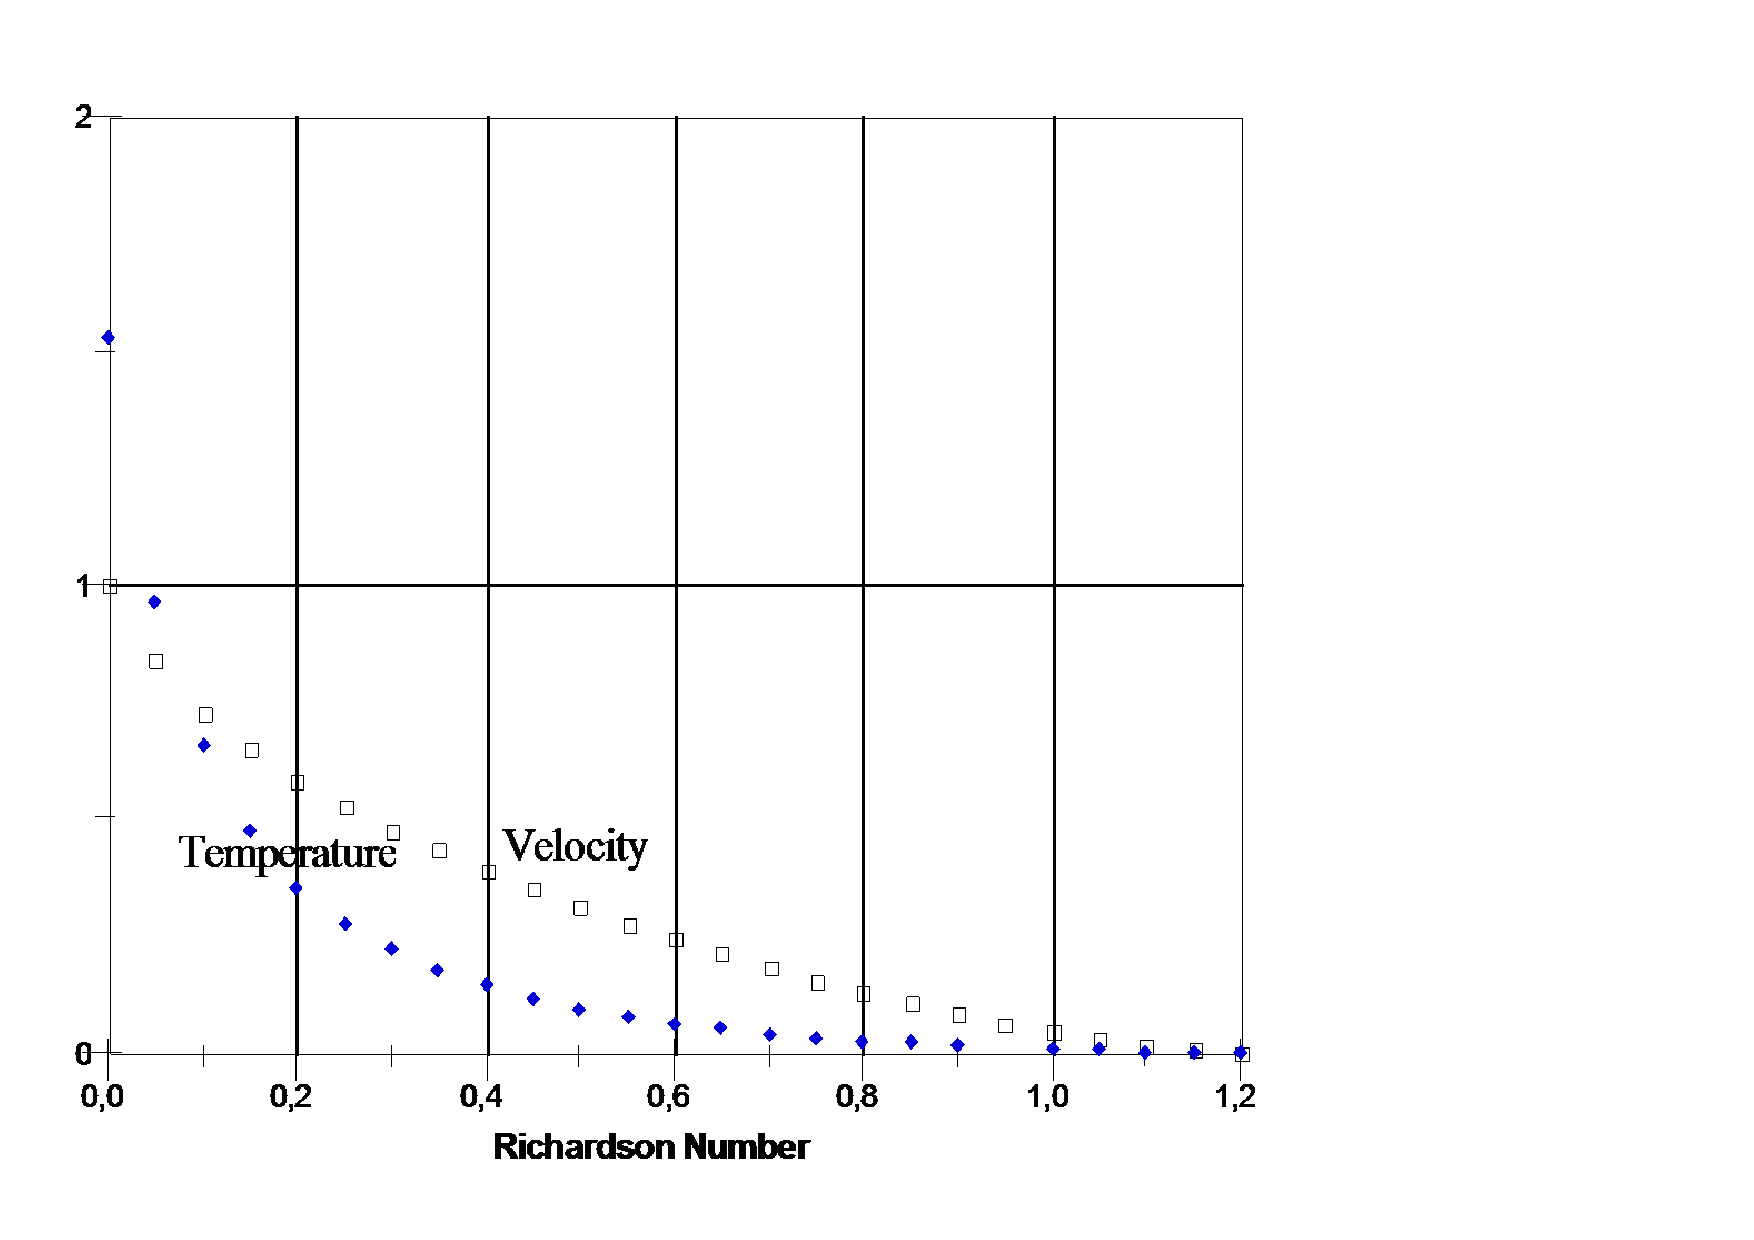
\includegraphics[scale = 0.5, trim=0 0 200 50, clip]{graphics/richardson.pdf}
  \caption{Damping functions on the velocity and scalar}
  \label{figure6}%
\end{figure}

The mixing length $L_{m}$ can be modelled in different ways:

\textbf{Classical} \textbf{Prandtl} \textbf{model} (see \cite{rodi84}):

$L_{m}=\kappa z$\ if $z\leq0.2h$ (here, $z$ is the distance to the bed and
$h$ the water depth).

$L_{m}=0.2\kappa h$\ if $z\geq0.2h$.

\textbf{Nezu and Nakagawa model} (see \cite{nezu93}):%

\[
L_{m}=\kappa z\sqrt{1-\dfrac{z}{h}}%
\]


In this case the mixing length vanishes at the free surface. This model can
give a logarithmic velocity profile from bed to free surface.

\textbf{Quetin} \textbf{model} (1977, see \cite{quetin77}):%
\index{Quetin model}%
%

\[
L_{m}=\dfrac{1}{\dfrac{1}{\kappa z}+\dfrac{1}{0.65d}}%
\]
where $d$ is the distance to the free surface.

\textbf{Tsanis model} (see \cite{tsanis89}):%
\index{Tsanis model}%


$L_{m}=\kappa z$\ if $z\leq0.2h$ (here, $z$ is the distance to the bed and
$h$ the water depth).

$L_{m}=0.2\kappa h$\ if $z\geq0.2h$ and $z\leq0.8h$.

$L_{m}=\kappa d$\ if $z\geq0.8h$ ($d$ is the distance to the free surface).

In the production of turbulence expression, the horizontal gradients of $u$
and $v$ as well as the gradients of $w$ are assumed negligible compared to the
vertical gradients. The term:
\[
\sqrt{\left(  \dfrac{\partial u}{\partial z}\right)  ^{2}+\left(
    \dfrac{\partial v}{\partial z}\right)  ^{2}}%
\]
is thus only an approximation of $\sqrt{2S_{ij}S_{ij}}$. For a calculation in
the vicinity of a structure (quay, spikes, etc.), the gradients overlooked
here can become important. However, their presence in the vertical viscosity
expression would not be of much help to perform an efficient calculation
around a structure. A mixing length model for horizontal viscosity would also
become necessary. Hence a precise computation of flow around structures is not
possible with this turbulence modelling.%



\subsubsection{\label{smagorinski}Smagorinski model%
  \index{Smagorinski model}%
}

The Smagorinski model (see \cite{smagorinski63}) has a meaning only in
numerical modelling and is based on the mixing length model. It belongs to the
category of sub-grid turbulence models. The principle is as follows:
turbulence is the solution of the Navier--Stokes equations. It would naturally
appear in the numerical solutions if the size of finite elements allowed the
reproduction of all mechanisms including the viscous dissipation of very small
vortices. Only in the formation of smaller vortices, where turbulence is
inhibited by the mesh, does modelling take place in a numerical simulation.
Smagorinski's idea is to add to the molecular viscosity a turbulent viscosity
deduced from a mixing length model. This mixing length corresponds to the size
of the vortices smaller than that of the mesh size. We simply arrive at the
following formulation:%

\begin{equation}
  \nu_T=C_{s}^{2}\Delta^{2}\sqrt{2S_{ij}S_{ij}}%
\end{equation}
where $C_{s}$ is a dimensionless coefficient to be calibrated and $\Delta$ the
mesh size derived in 2D or 3D from the surface or from the volume of the
elements. The values of $C_{s}$ range from 0.1 (flow in a canal) to 0.2
(isotropic turbulence). This model is best understood in 3D. In 2D it does not
take dispersion into account.


\subsection{\label{k-epsilon 3D}Two-equations $k$--$\epsilon$ model%
  \index{k--$\epsilon$ model|textbf}%
}

This model is based on the calculation of physical quantities representing
turbulence in the flow.
%$k$ and $\epsilon$ respectively designate turbulent
%kinetic energy%
%\index{turbulent kinetic energy}
%and its dissipation%
%\index{dissipation}%
%:%
%
%\begin{equation}
%  k=\dfrac{1}{2}\overline{u_{i}^{^{\prime}}u_{i}^{^{\prime}}}%
%\end{equation}
%%
%
%\begin{equation}
%  \epsilon=\nu\overline{\dfrac{\partial u_{i}^{^{\prime}}}{\partial x_{j}%
%    }\dfrac{\partial u_{i}^{^{\prime}}}{\partial x_{j}}}%
%\end{equation}
%where $u_{i}^{^{\prime}}$ is the turbulent fluctuation%
%\index{turbulent fluctuation}
%of velocity and where the bar represents averaging.

\subsubsection{$k$ and $\epsilon$ equations:}\label{sec:kepsequations}

The transport equation on $k$ is obtained by taking the trace of the transport equation on the Reynolds stresses, and reads:
\begin{equation}\label{eq:kEquation}
  \dfrac{\partial k}{\partial t} +\overline{\vec{u}}\cdot \Grad k= \mathbb P + \nabla \cdot \vec{Q}^k - \epsilon + \mathbb{G}
\end{equation}
where $\mathbb P$ is a production term whose definition is ~\mbox{$\mathbb P=-\vec{R}\!:\!\vec{S}$}.
By using the Boussinesq model~\eqref{eq:Boussinesq}, it can be written as%
\footnote{Strictly speaking, the term $-2/3 k \nabla \cdot \vec u$ should be taken into account for flows that are not truly incompressible.}:
\begin{equation}\label{eq:production}
  \mathbb P = \nu_T S^2
\end{equation}
with $S$ the scalar mean rate-of-strain defined as:
\begin{equation}\label{eq:scalarS}
  S = \sqrt{2\vec{S}:\vec{S}}
\end{equation}
$\mathbb{G}$ is a source term due to the forces of gravity in the case of temperature gradients.
It comes from the derivation of the Reynolds stress equation under the form: $\mathbb G = -\beta\vec{g}\cdot \overline{\vec{u}'T'}$, and thus also appears in the $k$ equation. This term is modelled through a turbulent thermal diffusivity model,
which yields:
\begin{equation}
\mathbb{G}=-\beta\dfrac{\nu_T}{Pr_T}g\dfrac{\partial \overline{T}}{\partial z}%
\end{equation}
with $\beta=-1/\rho(\partial\rho/\partial \overline{T})$, $Pr_T$ being the turbulent
Prandtl number.\index{Prandtl}%
In~\eqref{eq:kEquation}, $\vec{Q}^k$ is the flux of $k$, which represents a transport of
kinetic and potential energy by the eddies and the molecular viscosity.
The flux of $k$ can be modelled through a diffusion term:
\begin{equation}
  \nabla \cdot \vec{Q}^k = \dfrac{1}{\rho}\nabla \cdot \left(\mu_k \vec \nabla k\right)
\end{equation}
where $\mu_k$ is defined as $\mu_k = \mu+\mu_T/\sigma_k$, $\sigma_k$ being a model constant.
On the other hand, $\epsilon$ corresponds to a dissipation of turbulent kinetic energy (transformed into thermal energy) due to the viscosity, defined as:
\begin{equation}
  \epsilon = \nu \sum_i\sum_j\overline{\left(\dfrac{\partial u'_i}{\partial x_j}\right)^2}
\end{equation}
where $\partial u'_i/\partial x_j$  denotes the derivative of the $i$th component of $\vec u'$ with respect to the $j$th coordinate.
Although it is possible to write an exact transport equation on $\epsilon$, the latter includes complex terms that cannot be explicitly calculated.
This is why, in the $k-\epsilon$ model $\epsilon$ is computed through a simplified equation that reproduces the $k$ equation:
\begin{equation}\label{eq:epsilonEquation}
  \dfrac{\partial\epsilon}{\partial t}+\overline{\vec{u}}\cdot \Grad \epsilon =
C_{1\epsilon}\dfrac{\epsilon}{k}\left(\mathbb P+(1-C_{3\epsilon})\mathbb G\right)  -C_{2\epsilon}\dfrac{\epsilon^2}{k}
+ \dfrac{1}{\rho}\Div \left(\mu_\epsilon \vec \nabla \epsilon\right)
\end{equation}
where $\mu_\epsilon$ is defined as: $\mu_\epsilon = \mu+\mu_T/\sigma_\epsilon$, $\sigma_\epsilon$ being a constant.
$C_{1\epsilon}$ and $C_{2\epsilon}$ are also constants of the model (see the table~\ref{epsilon}).
The equation~\eqref{eq:epsilonEquation} has no theoretical background but relies on empirical considerations. The constant $C_{3\epsilon}$ was introduced in order to represent the fact that stable stratifications
weaken turbulence. It is thus taken as equal to one if $\mathbb G$ is negative, and zero otherwise.
The term $\epsilon/k$ is the frequency of the large eddies, it ensures the equation homogeneity.
The $\epsilon$ source terms are supposed proportional to the ones in the $k$ equation.\\

Note that the $k-\epsilon$ model is not accurate concerning non-inertial and streamline curvature effects, as well as severe deviation from local equilibrium.
Besides, it was shown that computing the production term through~\eqref{eq:production} leads to over-estimations of $k$ and thus of $\nu_T$.
In order to avoid this, Guimet \& Laurence~\cite{Guimet2002} proposed to restrict the production term to a linear behaviour for high values of the rate-of-strain,
obtained from the equilibrium between $\mathbb P$ and $\epsilon$ for fully developed homogeneous turbulence.
This yields a linear-quadratic model for the production%
\footnote{This essentially recovers the SST modification~\cite{Menter1994}, although it does not include a low-Reynolds treatment.}:
\begin{equation}\label{eq:P}
\mathbb P = \text{min}\left(\sqrt{C_\mu} k S, \nu_T S^2 \right)
\end{equation}
Another issue is that the size of the large eddies, given by $L_t \sim k^{3/2}/\epsilon$, may be predicted arbitrarily large, which is not physical since $L_t$ should
be bounded at least by $L$, the characteristic size of the flow.
To remedy this issue, Yap~\cite{Yap1987} proposed a modification of the $C_{2\epsilon}$ coefficient in order to increase the dissipation of turbulent kinetic energy:
\begin{equation}\label{eq:Cepsilon2_Yap}
  C_{2\epsilon,Y} = \text{max}\left(C_{2\epsilon} - \text{max}\left[ 0, 0.83\left(\dfrac{L_t}{L}-1\right)\left(\dfrac{L_t}{L}\right)^2 \right],0\right)
\end{equation}

\begin{CommentBlock}{Remark:}
By default the Yap treatment for $C_{2\epsilon}$ is not activated in \telemac{3d}.
This choice of option is hard-coded in the routine CSTKEP.f at the line 183.
\end{CommentBlock}

The Kolmogorov dimensional analysis~\cite{Kolmogorov1991} leads to a definition of the eddy viscosity as a function of $k$ and $\epsilon$,
which corresponds to the fact that the large turbulent eddies are the ones that most interact with the mean flow.
$\nu_T$ is thus written as proportional to the length scale of the large eddies, $L_t \sim k^{3/2}/\epsilon$, which yields:
\begin{equation}\label{eq:nut}
\nu_T = C_\mu \dfrac{k^2}{\epsilon}
\end{equation}
$C_\mu$ is the Prandtl-Kolmogorov constant.\\

The constants of the $k$--$\epsilon$ model have been determined by
comparison with simple situations. The constants $C_{\mu}$ and
$C_{1\epsilon}$ are obtained from data for turbulent flow near a rigid
wall. The free decay of grid turbulence helps us to find a value for
$C_{2\epsilon}$ on the basis of well-documented experimental data. The
constants $\sigma_{k}$ and $\sigma_{\epsilon}$ have been \textquotedblleft
optimised\textquotedblright, based on the performance of the model in both the
test cases just mentioned. Obtaining $C_{3\epsilon} $ is elaborated in
references \cite{launder74} and \cite{Viollet2002}. We retain that
$C_{3\epsilon}$ is equal to 1 for a stable situation, i.e. if $\mathbb G$ is
negative, and equal to 0 for unstable stratifications. $\sigma_{k}$ is
sometimes called \textquotedblleft Prandtl's turbulent number for the kinetic
energy of turbulence\textquotedblright.
All these constants are summarised in the table \ref{epsilon}.%

\textbf{Remarks:}
\begin{itemize}
\item {It is the equilibrium hypothesis between the creation of turbulence and
dissipation which leads to the mixing length model%
\index{mixing length model}%
. Actually, by assuming $\mathbb P=\epsilon$, and as $\nu_T\approx k^{2}/\epsilon$,
we immediately find $\nu_T\approx k^{2}/\mathbb P$. Also
$\nu_T\approx\sqrt{k}L_{t}$, where $L_{t}$ is the characteristic size of
vortices. We get:
\[\nu_T^{2}\approx\dfrac{k^{2}}{2S_{ij}S_{ij}}\]
and $\nu_T^{4}\approx k^{2}L_{t}^{4}$. By dividing the second equation by
the first one, member by member, we finally get:%

\[\nu_T\approx L_{t}^{2}\sqrt{2S_{ij}S_{ij}}\]
}
\item{In internal flow modelling, the term $-2/3 \, k\,\delta_{ij}$ is often
omitted because it plays the same role as pressure. If we want to have the
true pressure, it is not possible to integrate this term which should thus
appear in numerical resolution.
}
\end{itemize}

\begin{table}[tbp] \centering
  \caption{constants of the $k$--$\epsilon $ model  \label{epsilon}}$%
  \begin{tabular}
    [c]{|c|c|c|c|c|c|c|c|}\hline
    $\kappa$ & $C_\mu$ & $Pr_T$ & $C_{1\epsilon}$ & $C_{2\epsilon}$ &
    $C_{3\epsilon}$ & $\sigma_{k}$ & $\sigma_{\epsilon}$\\\hline
    0.41 & 0.09 & 1.0 & 1.44 & 1.92 & 0 if $\mathbb G>$ 0 and 1 if $\mathbb G\leq$ 0 & 1.0 &
    1.3\\\hline
  \end{tabular}
  \ $%
\end{table}%


\paragraph{\label{k-epsilon limites}Boundary conditions of the $k$%
  --$\epsilon$ model}

\paragraph{Rigid boundaries:}

to define rigid boundary conditions%
\index{boundary conditions!$k$--$\epsilon$ model},
it is considered that turbulence is in local equilibrium at the wall, such
that the production of turbulence (due to shear at the wall and at the bed)
is equal to dissipation and the velocity profile is locally logarithmic. This
idea was exploited by Mellor and Yamada to establish a zero-equation
turbulence model (see \cite{mellor74}).
With the equilibrium hypothesis, at a distance $\delta$ from the wall, the
$k$--$\epsilon$ model equations are:
\begin{equation}
  k=\dfrac{u_\ast^{2}}{\sqrt{C_{\mu}}}
\end{equation}

\begin{equation}
  \epsilon=\dfrac{u_\ast^{3}}{\kappa \delta}%
\end{equation}
The distance $\delta$ is chosen equal to 1/10th of the local mesh size,
measured along the normal direction to the wall. In the presence of
turbulence, the boundary condition for velocity is now written as:
\begin{equation}
\nu_T\dfrac{\partial u}{\partial n}=-u_\ast^{2}%
\end{equation}
$\nu$ being replaced by $\nu_T$.

\paragraph{Liquid boundaries:}

without additional information on the value of $k$ and $\epsilon$ at a
liquid boundary, a \textquotedblleft weak\textquotedblright\ condition is
applied, i.e. $\nu_T(\partial k/\partial n)=0$ and
$\nu_T(\partial\epsilon/\partial n)=0$. Such a condition can, however, give
rise to numerical problems at the entrance of a domain.

\paragraph{Free-surface:}
The treatment of boundary conditions on $k$ and $\epsilon$ at the free-surface
is tricky since it is not clear what to do in this case.
In \telemac{3d}, the following is done:
\begin{itemize}
\item the production term is considered quadratic at the free-surface:
\begin{equation}
\mathbb{P}=\nu_TS^2
\end{equation}
\item $\nu_T$ is calculated through the formula \eqref{eq:nut} but with a specific value of $k$.
The later is calculated based on the definition of the friction
velocity at the free-surface (obtained from the equation \eqref{eq:windstress}):
\begin{equation}
u_\ast|_{z=\eta}=\sqrt{a_{wind}\rho_{air}/\rho}~u_{wind}
\end{equation}
and considering that $k$ is defined by $k=u_\ast^2/\sqrt{C_\mu}$. The value
of $k$ at the free-surface is thus taken as:
\begin{equation}
k|_{z=\eta}=\left(\dfrac{a_{wind}\rho_{air}u_{wind}^2/\rho}{\sqrt{C_\mu}}\right)^2
\end{equation}
\end{itemize}

\begin{CommentBlock}{Remark:}
In the absence of wind the boundary condition on $k$ and $\epsilon$
at the free-surface is a zero-gradient.
However, the presence of the free-surface should reduce the length scale of the large eddies \cite{Hunt1984}.
A possibility to take this effect into account is to use the boundary condition on $\epsilon$
proposed in \cite{Celik1984}:
\begin{equation}
\epsilon_\eta=\dfrac{k_\eta^{3/2}}{\alpha h}
\end{equation}
where $\alpha \approx 0.18$ is an empirical constant, $k_\eta$ and $\epsilon_\eta$ are
the values of $k$ and $\epsilon$ at the free-surface and $h$ is the water depth.
\end{CommentBlock}

\subsection{Other models}

Though sufficiently difficult to implement numerically, the $k$--$\epsilon$
model has obvious limitations, particularly for eddies behind obstacles and in
the presence of a high rate of deformation (tensor $S_{ij}$) near a stagnation
point, for example. The Reynolds Stress Model (RSM) is a higher order model. The six
Reynolds stress%
\index{Reynolds!stress}
equations are then directly solved, and the $\epsilon$ equation, together
with the equations of scalar turbulent flux of temperature and salinity. Only
this type of model is capable of really taking into account turbulence
anisotropy by dropping the Boussinesq model. However, the triple
correlations of the equations are difficult to model and the boundary
conditions difficult to justify. This model has not been implemented in \telemac{3d} yet.
% To our knowledge, this is the reason why
% there is still no industry-oriented application of this model in free surface hydrodynamics.

\subsection{\label{contraintes turbulentes}Turbulent stress on the walls}

The presence of walls in turbulent flows makes the
latter anisotropic and increases the production of turbulence due to shearing effects.
Modelling near-wall turbulence is crucial in order to correctly reproduce the flows,
since the no-slip condition leads to large values of the velocity gradient at the walls,
which generates turbulence.
Let us denote by $y$ the distance to a wall and $y^+$ the dimensionless distance to a wall, defined as:
\begin{equation}\label{eq:yPlus}
  y^+=\dfrac{y u_*}{\nu}
\end{equation}
with $u_*$ a friction velocity, defined by:
\begin{equation}
  -\rho u_*^2\dfrac{\vec{u}_\tau}{u_\tau} = \vec{\tau} = \mu \left.\dfrac{\partial \vec{u}_\tau}{\partial y}\right|_{y=0}
\end{equation}
where $\vec{u}_\tau$ is the tangential velocity to the wall, $u_\tau$ its norm and $\vec{\tau}$ is the shear-stress,
with units \mbox{kg m$^{-1}$s$^{-2}$}.
The observation of the turbulent flow between two horizontal parallel plane walls (this configuration is called the plane Poiseuille channel)
led to a sub-division of the near-wall region into three areas~\cite{Viollet2002}:
\begin{itemize}
\item the viscous sub-layer: $0<y^+<8$
\item the buffer layer: $8<y^+<30$
\item the inertial sub-layer: $30<y^+<0.2e^+$
\end{itemize}
where $e^+$ is the dimensionless half-height of the channel, defined by $e^+=e u_{*}/\nu$ with $e$ the half-height.
The turbulence is negligible in the viscous sub-layer while the viscous effects are small in the inertial sub-layer.
In the latter, the velocity profile distribution along the normal to the wall follows a logarithmic law, so that this zone is also called the logarithmic zone.
If the characteristic roughness size of the wall is greater
than the thickness of the viscous sub-layer, this viscous sub-layer cannot
develop and the flow is known to be hydraulically rough. If there is a viscous
sub-layer the flow is known to be hydraulically smooth.
%To describe the velocity profile
%in the different layers, we consider a 1D flow for the sake of simplicity.
In the inertial layer, the velocity profile takes the following form:\\

\textbf{For hydraulically smooth flow:}\index{smooth flow}
\begin{equation}
  \dfrac{u_\tau}{u_*}=\dfrac{1}{\kappa}\ln\left(y^+\right)+5.2 \label{logarsmooth}
\end{equation}
For hydraulically smooth flow the linear and logarithmic laws are unified by
the Reichard law:
\begin{equation}
  \dfrac{u_\tau}{u_*}=\dfrac{1}{\kappa}\ln(1+\kappa y^{+})+7.8(1-e^{-\dfrac{y^{+}%
    }{11}})-\dfrac{y^{+}}{11}e^{-0.33y^{+}} \label{REICHARD}%
\end{equation}

\textbf{For hydraulically rough flow:}\index{rough flow}
\begin{equation}\label{eq:logarrough}
  \dfrac{u_\tau}{u_*}=\dfrac{1}{\kappa}\ln\left(  \dfrac{33 y}{k_{s}}\right)
  =\dfrac{1}{\kappa}\ln\left(  \dfrac{y}{k_{s}}\right)  +8.5
\end{equation}
where $k_{s}$ is the roughness size.
An equivalent way of writing the velocity profile for the hydraulically rough
flow is:%
\begin{equation}
  \dfrac{u_\tau}{u_*}=\dfrac{1}{\kappa}\ln\left(  \dfrac{y}{y_{o}}\right)
  \label{logarrough}%
\end{equation}
where$\;y_{o}\approx k_{s}/33$.
The reference \cite{Viollet2002} contains theoretical justifications of these formulae.\\

Directly simulating near-wall turbulence requires very fine
meshes and modified turbulence models (so-called low-Reynolds turbulence models).
Then, the computational points closest to the wall must be located in the viscous sub-layer.
This is computationally expensive, especially for flows with high-Reynolds numbers.
This led to the development of wall functions, based on semi-empirical formulae,
which are used to reproduce near-wall effects with coarser discretisations.
This corresponds to high-Reynolds-number turbulence models and requires
the computational points closest to the wall to be located in the inertial layer.
% Since RANS models were designed in order to coarsen the space-time discretisation, a wall boundary model is required in
% order to reproduce the effects of near-wall turbulence.
In Eulerian models, this can be done by designing the mesh so that
the first calculation point is in the logarithmic zone.
Another possibility is to solve the discretised equations
on a~'classical'~mesh, where the nodes located on the wall
are treated in the same way as if they were shifted in the
normal direction so as to be in the logarithmic zone, as for instance in~\cite{Kuzmin2007}.
%This makes it possible to resolve the region with more than one or two points.
This is done in \telemac{3d}: the velocity at the wall is taken in the boundary layer at a distance $y$.
$y$ is arbitrarily chosen or made to depend on the local mesh size
(\textit{e.g.} the edge point is at a distance from
the real wall equal to 1/10th of the size of the mesh).
Then, it is possible to specify the laws to be adopted in numerical
simulations to compute $u_*$ at the walls.
%In \telemac{3d}, only the case of hydraulically rough flows
%is considered (since in environmental flows, smooth regimes are
%hardly ever encountered).

\subsubsection{Hydraulically smooth flow%
  \index{smooth flow}%
}
By knowing $u_\tau$ and
$y$, the Reichard law (Equation \ref{REICHARD})\ gives $u_*$ from the
formula:
\index{Reichard law}
\begin{equation}
  \dfrac{u_*}{u_\tau}=\dfrac{1}{\dfrac{1}{\kappa}\ln(1+\kappa y^{+}%
    )+7.8(1-e^{-\dfrac{y^{+}}{11}})-\dfrac{y^{+}}{11}e^{-0.33y^{+}}}%
\end{equation}
This law is implicit as $y^{+}$\ depends on $u_*$, and $u_*$ is
found by successive iterations (10 iterations are done).
We then write:
\begin{equation}
  \nu\dfrac{\partial u_\tau}{\partial n}=-u_*{}^{2}%
\end{equation}

\subsubsection{Hydraulically rough flow}
Dimensional analysis
shows that $\vec{\tau}$ has the form:
\begin{equation}
\vec{\tau}=-\dfrac{1}{2}\rho C_{f}\vec{u}_\tau\vec{u}_\tau
\end{equation}
where $C_{f}$ is a dimensionless friction
coefficient. This general formula for shear forces supposes that
$\vec{u}_\tau$ is sufficiently far from the wall. It can also be written
as:
\begin{equation}
  \mu\dfrac{\partial\vec{u}_\tau}{\partial \vec{n}}=-\dfrac{1}{2}\rho C_{f}\vec{u}_\tau\vec{u}_\tau%
\end{equation}

The specification of the stress $\mu\partial\vec{u}_\tau / \partial \vec{n}$ will naturally appear in
the variational formulation of the diffusion terms in finite elements.
The bed shear stress condition will thus be ensured:
\begin{itemize}
\item Either by a turbulence model which will provide a formula for the stress
  $\mu (\partial\vec{u}_\tau / \partial \vec{n}$, based on the expression of
  the roughness at the bed and flow in the vicinity of the bed. Most
  often, the turbulence model gives the shear velocity $u_{\ast}$, or the
  friction coefficient $C_{f}$.

\item Or by knowledge of a friction coefficient $C_{f}$ and its associated
  velocity $\vec{u}_\tau$, which, due to the laws of bed shear stress
  in two dimensions, will be the average velocity on the vertical (the friction
  coefficients on the bed will thus be the same in two and three dimensions).
  This is the case of the Ch\'{e}zy, Strickler and Manning formulae:

  \textbf{Ch\'{e}zy formula:}%
  \index{Ch\'{e}zy!formula|textbf}
  ($C$ is the Ch\'{e}zy coefficient):%
  \begin{equation}
    C_{f}=\dfrac{2g}{C^{2}}%
  \end{equation}

  \textbf{Strickler formula:}%
  \index{Strickler!formula|textbf}
  ($S$ is the Strickler coefficient):%
  \begin{equation}
    C_{f}=\dfrac{2g}{h^{1/3}S^{2}}%
  \end{equation}

  \textbf{Manning formula:}%
  \index{Manning!formula}
  ($m$ is the Manning coefficient, equal to the inverse of the Strickler coefficient):%
  \begin{equation}
    C_{f}=\dfrac{2g\,m^{2}}{h^{1/3}}%
  \end{equation}
\end{itemize}
%In Section
%\ref{sec:solidBoundaries}\
%We have examined the Ch\'{e}zy, Strickler and Manning formulae.
%and Nikuradse formulae. For Nikuradse formula%
%\index{Nikuradse formula}%
%, we can now understand how it stems from the Ch\'{e}zy law and an integration
%vertically of the logarithmic profile given in Equation \eqref{eq:logarrough}.
When the roughness size $k_{s}$ is known, the following laws can also be used:\\

\textbf{Nikuradse formula:}%
\index{Nikuradse!formula}
This law stems from a depth-averaged value of the logarithmic turbulent velocity profile \eqref{eq:logarrough}.
The corresponding Chézy coefficient is obtained by the formula:%
\begin{equation}
  C=7.83\text{ln}\left(12\dfrac{h}{k_s}\right)
\end{equation}

\textbf{Haaland formula:}
\begin{equation}
  C_{f}=\dfrac{1}{4\left[0.6\ln\left(\left(\dfrac{6.9\nu}{4h\sqrt
            {u^{2}+v^{2}}}\right)^{3}+\dfrac{k_{s}}{14.8h}\right)\right]^{2}}
\end{equation}
\textbf{Ramette formula:}
according to Ramette \cite{ramette81}, the roughness size $k_{s}$ can also be
connected to the Ch\'{e}zy coefficient%
\index{Ch\'{e}zy!coefficient}
$C$ by the expression:
\begin{equation}
  C = \dfrac{26.4}{k_{s}^{1/6}}\left(\dfrac{k_{s}}{h}\right)^{1/24}h^{1/6}
\end{equation}
This last empirical formula is not dimensionless and requires a strict respect
of IS units.\\

\begin{CommentBlock}{Remark:}
In \telemac{3d}, there are options relying on the prescription of a friction coefficient,
with association to the depth-averaged velocity, because it seemed important to be able to
build a 3D model based on a 2D model without changing the calibration -- the Haaland, Chézy,
Strickler and Manning options. The Nikuradse
option, on the other hand, makes it possible to prescribe a friction based on a logarithmic
velocity profile for a given bed roughness, without any averaging of the velocity along the vertical.
It thus seems more appropriate than the depth-averaged models for the simulation of non quasi-horizontal flows.
\end{CommentBlock}
\newpage
\begin{CommentBlock}{Possible improvement for active scalars modelling:}
%\subsubsection{Turbulent boundary conditions on the temperature}
At the moment, in \telemac{3d} there is no treatment for the temperature boundary condition
when a Dirichlet condition is prescribed.
However, the temperature gradients close to the walls may be large in
turbulent mode, which generates turbulence as in the case of the velocity gradients.
If one were to consider applications where the scalar come close to a solid boundary,
it would be necessary to impose a wall function on the temperature with the $k-\epsilon$ model.
This is probably marginal but nevetheles the formulation is reported here.
Considering a 1-D fully developed flow field and thermal field in a channel,
the integration of the temperature equation along the normal to the wall,
from the wall to the centre of the channel reads:
\begin{equation}
  -Q_w = K_T \dfrac{d\overline T}{dy}
\end{equation}
where $y$ is the normal distance to the wall and $Q_w$ the heat flux applied at the wall.
Integrating once more yields:
\begin{equation}\label{eq:temperatureIntegral}
  \int_{T_w}^{\overline T} d\overline T = - Q_w \int_0^y\dfrac{dy}{K_T}
\end{equation}
where $T_w$ is the wall temperature. Defining the dimensionless variable
$T^+ = (T_w-\overline T)u_*/Q_w$, the equation~\eqref{eq:temperatureIntegral} can be written as:
\begin{equation}
  T^+ = \int_0^{y^+}\dfrac{\nu dy^+}{K_T}
\end{equation}
where $y^+$ is defined by~\eqref{eq:yPlus}. The integration of this equation can be done assuming a decomposition of the near-wall region into a laminar layer where $T^+$ varies linearly with $y^+$ and a turbulent layer where it follows a logarithmic law, as in~\cite{Bredberg2000}. It is also possible to use a three-layers model (see~\cite{Code_Saturne}) through:
\begin{equation}\label{eq:Tplus}
  \left\{\begin{array}{ll}
      T^+=Pr\hspace{0.05cm}y^+ & \text{if}~ y^+<y_1^+ \smallskip \\
      T^+=a_2-\dfrac{Pr_T}{2 a_1 \left(y^+\right)^2} &  \text{if}~ y_1^+ \le y^+<y_2^+ \smallskip \\
      T^+=\dfrac{Pr_T}{\kappa}\text{ln}~y^++a_3 &  \text{if}~ y^+>y_2^+ \smallskip \\
    \end{array}\right.
\end{equation}
where the following constants were defined:
\begin{equation}\label{eq:Tplus_constants}
  \left\{\begin{array}{l}
      y_1^+ = \left(\dfrac{a_{4}}{Pr}\right)^{1/3}~,~~~ y_2^+ = \sqrt{\dfrac{a_{4}\kappa}{Pr_T}}~,~~~a_1 = \dfrac{Pr_T}{a_{4}}, \smallskip \\
      a_2 = 15 Pr^{2/3}~,~~~a_3 = 15 Pr^{2/3} - \dfrac{Pr_T}{2\kappa}\left(1+\text{ln}~\dfrac{a_{4}\kappa}{Pr_T}\right)~,~~~ a_{4}=1000
    \end{array}\right.
\end{equation}
Recall that $\kappa$ is defined in the table~\ref{epsilon} and $Pr_T$ is the turbulent Prandtl number. Finally, $Pr=\dfrac{\nu}{K}$ is the molecular Prandtl number.
\end{CommentBlock}
%At the free-surface a homogeneous Neumann condition is imposed (no heat-flux).
%On the other hand, at inflow boundaries a Dirichlet condition is set on the temperature, whereas at outflow boundaries
%a homogeneous Neumann condition is prescribed (like for $k$ and $\epsilon$).
%%%%%%%%%%%%%%%%%%%%%%%%%%%%%%%%%%%%%%%%%%%%%%

\section{Modelling culverts in the flow}

\subsection{An example of application: a flood control area in the Scheldt estuary}

Flood Control Areas (FCA) together with a Controlled Reduced Tide (CRT) system
are implemented in the Scheldt estuary to reduce the risk of flooding.
The former is defined by an area specifically located in the regions where
the bottom elevation is lower than the mean tide elevation.
This area is surrounded by an outer higher dyke and in the interface with the river,
it has a lower dyke that allows the flow to overtop the structure during storm surges.
The CRT is based on the construction of inlet and outlet sluices that control the
flow between the river and the floodplain depending on the water levels on both
sides (see the figure \ref{fig:culvert_fig1}) \cite{Teles2015}.

\begin{figure}[H]
\begin{center}
  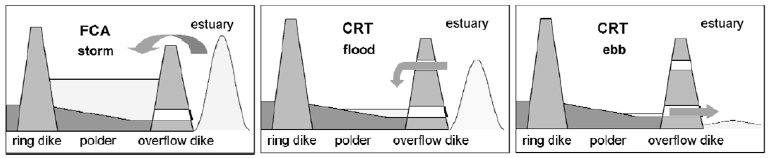
\includegraphics[width=0.95\textwidth]{graphics/culvert_fig1.png}
\end{center}
\caption{Water movements between the FCA and river without
CRT (on the left) and with CRT (on the middle and right pannels).
(Source: De Mulder et al. (2013)).}
\label{fig:culvert_fig1}
\end{figure}

The incorporation of these structures in numerical models is essential
to better predict and describe the flow hydrodynamics going to and
coming from these areas. The inlet and outlet sluices act like a weir
when they are not fully submerged and when water levels rise above the
inlet ceiling pressurised flow formulae are used.
The calibration of the head loss coefficients for the inlet and outlet sluices
was done comparing model results with measured water levels and discharges of
one specific CFA/CRT, called Lippenbroek.
Later these values were validated using the measurements from the CFA/CRT Bergenmeersen.
The coefficients found in this calibration/validation exercise are used for all the
other inlet and outlet sluices for the other FCA, FCA/CRT areas in the 3D model.

\subsection{Flow through a culvert: theoretical background}

A number of studies regarding the description of flows through the culverts
refer to Bodhaine's work \cite{Bodhaine1968}.
Bodhaine categorized the flow through a culvert into six types, and for each type
the discharge is calculated in a different way.
The equations are deduced from the continuity and energy equations between the approach
section (see the figure \ref{fig:culvert_fig2}) and the exit (downstream) section of the culvert.
The type of flow depends on whether the culvert flows full and whether the flow is controlled
by the entrance or exit part of the culvert. The figure \ref{fig:culvert_fig2}
shows a sketch for culvert flow definition.

\begin{figure}[H]
\begin{center}
  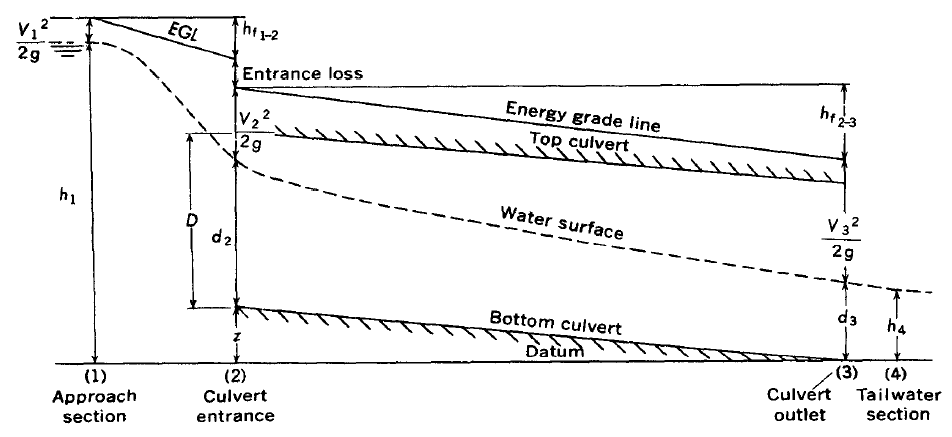
\includegraphics[width=0.95\textwidth]{graphics/culvert_fig2.png}
\end{center}
\caption{Sketch of general flow through a culvert \cite{Bodhaine1968}.}
\label{fig:culvert_fig2}
\end{figure}

$Z$ gives the elevation of the culvert entrance relative to the datum through the culvert exit.
The gravitational constant is given by $g$ and $h_{f12}$ is the head loss due to friction from
the approach section to the culvert entrance;
$h_{f23}$ is the head loss due to friction inside the culvert, $d_2$ and $d_3$ are the water
depths at the culvert entrance and exit, respectively;
$V_1$, $V_2$ and $V_3$ are the velocities at the approach section,
culvert entrance and culvert exit, respectively;
$D$ is the culvert height;
and $h_1$ and $h_4$ are the water depths upstream and downstream of the culvert structure.
The six types of flow classified by Bodhaine \cite{Bodhaine1968} depend on the water depths
upstream and downstream of the culvert.
The figure \ref{fig:culvert_fig3} gives a schematization of the different flow types
made according to the equation for each type of flow.
The different equations are presented below.

\begin{figure}[H]
\begin{center}
  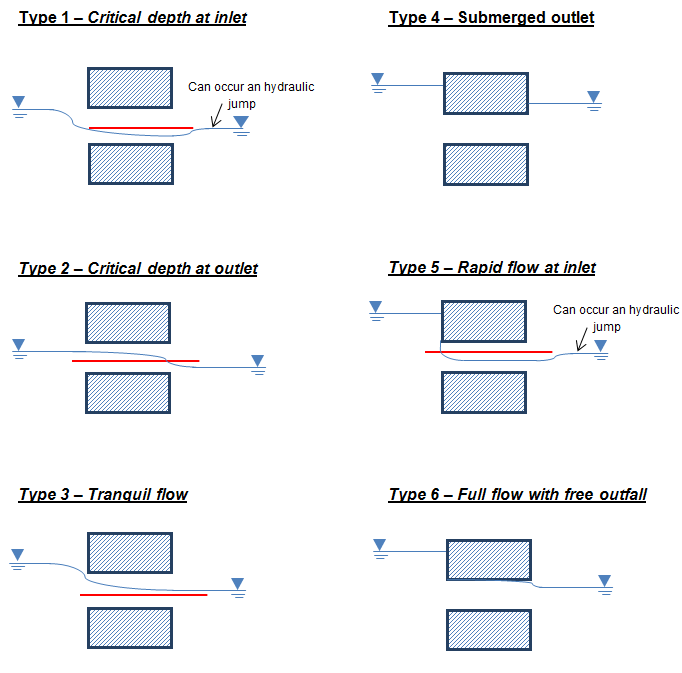
\includegraphics[width=0.7\textwidth]{graphics/culvert_fig3.png}
\end{center}
\caption{Sketch of the 6 different types of flow that occur
through culverts according to Bodhaine \cite{Bodhaine1968}.
The red line represents the critical water depth.}
\label{fig:culvert_fig3}
\end{figure}

\underline{\textbf{Type 1 -- Critical depth at inlet- supercritical flow at the entrance}}\\

In flow type 1 the flow is supercritical inside the culvert and the critical depth occurs
at the entrance of the culvert. The culvert slope ($S_0$) has to be greater than the
critical slope ($S_c$) and the culvert flows partially full.
For the Froude number $Fr=1$ (which is the case of flow type 1),
the discharge coefficient is typically $C_D=0.95$.
The discharge is then calculated according to the following formula:

\begin{equation}
Q = C_D A_c \sqrt{2g\left(h_1-z-h_c-h_{f12}+\alpha \dfrac{\overline{V_1}^2}{2g}\right)}
\end{equation}

with:\\
$C_D$ the discharge coefficient;\\
$A_c$ the flow area at critical water depth; \\
$g$ the gravitational constant; \\
$h_1$ the upstream water depth; \\
$z$ elevation of the culvert entrance; \\
$h_c$ the critical water depth; \\
$h_{f12}$ the head loss due to friction from the approach section to the culvert entrance; \\
$\alpha$ the kinetic energy correction coefficient for the approach section; \\
$V_1$ the average flow velocity at the approach section of the culvert.\\

\underline{\textbf{Type 2 -- Critical depth at outlet – supercritical flow at the exit}}\\

In flow type 2 the flow is tranquil inside the culvert. The critical depth is located at
the culvert outlet. The culvert flows partially full. Here the culvert slope has to be
smaller than the critical slope. The discharge coefficient is similar to flow type 1.
The discharge is then calculated according to the following formula:
\begin{equation}
Q=C_D A_c \sqrt{2g\left(h_1-h_c-h_{f12}-h_{f23}+\alpha \dfrac{\overline{V_1}^2}{2g}\right)}
\end{equation}
with:\\
$h_{f23}$ the head loss due to friction inside the culvert.\\

\underline{\textbf{Type 3 -- Tranquil flow -- subcritical flow}}\\

In flow type 3 the flow is subcritical inside the culvert. There is no critical depth.
The culvert flows partially full. Like flow types 1 and 2, the discharge coefficient
varies with respect to the Froude number, being typically between $C_D=0.82 -- 0.95$.
The discharge is calculated according to the following formula:
\begin{equation}
Q=C_D A_3 \sqrt{2g\left(h_1-d_3-h_{f12}-h_{f23}+\alpha \dfrac{\overline{V_1}^2}{2g}\right)}
\end{equation}
with:\\
$A_3$ the flow area at the culvert outlet;\\
$d_3$ the water depth at the culvert outlet.\\

\underline{\textbf{Type 4 -- Submerged inlet and outlet}}\\

In flow type 4 the culvert inlet and outlet are submerged. The culvert flows full.
The discharge coefficient varies with respect to the culvert geometry, ranging
typically between $C_D=0.75$ and $C_D=0.95$.
The discharge is calculated according to the following formula:
\begin{equation}
Q=C_D A_0 \sqrt{2g\dfrac{h_1-h_4}{1+29C_D^2 n^2 L/R^{4/3}}}
\end{equation}
with:\\
$A_0$ the flow area at the culvert entrance;\\
$h_4$ the downstream water depth;\\
$n$ the Manning coefficient;\\
$L$ the length of the culvert;\\
$R$ the hydraulic radius.\\

\underline{\textbf{Type 5 -- Rapid flow at inlet}}\\

In flow type 5, the flow is supercritical at the inlet to the culvert.
The culvert flows partially full. Type 5 flow does not usually occur.
When it does, the discharge coefficient is in general lower than the other types.
\begin{equation}
Q=C_D A_0 \sqrt{2g(h_1-z)}
\end{equation}

\underline{\textbf{Type 6 -- Full flow with free outfall}}\\

In flow type 6 the culvert flows full. The discharge coefficient is similar to the
one obtained for the flow type 4.
The discharge is calculated according to the following formula:
\begin{equation}
Q=C_D A_0 \sqrt{2g(h_1-d_3-h_{f23})}
\end{equation}
The indices of the different variables might seem a bit confusing,
but it was chosen to take the formulae from Bodhaine as they were
and not to make any changes to them.
Bodhaine differentiated between these six flow types based on conditions
given in the table \ref{tab:culvert_tab1}.

\begin{table}[H]
\caption{Conditions for each type of flow defined by Bodhaine \cite{Bodhaine1968}.}\label{tab:culvert_tab1}
\begin{center}\begin{tabular}{|c|c|c|c|}
\hline
~ & $\mathbf{\dfrac{h_1-z}{D}}$ & ~ & ~\\
\hline
\textbf{Type 1} & $<1.5$    &  $\frac{h_4}{h_c} < 1.0$ & $S_0 > S_c$\\
\hline
\textbf{Type 2} & $<1.5$    &  $\frac{h_4}{h_c} > 1.0$ & $S_0 < S_c$\\
\hline
\textbf{Type 3} & $<1.5$    & $\frac{h_4}{D} \le 1.0$ & ~\\
\hline
\textbf{Type 4} & $> 1.0$   & $\frac{h_4}{D} > 1.0$ & ~\\
\hline
\textbf{Type 5} & $\ge 1.5$ & $\frac{h_4}{D} \le 1.0$ & ~\\
\hline
\textbf{Type 6} & $\ge 1.5$ & $\frac{h_4}{D} > 1.0$  & ~\\
\hline
\end{tabular}\end{center}
\end{table}

All the different culvert geometric features will affect the presence of culvert flow type 5 or 6.
To differentiate the two types, Bodhaine \cite{Bodhaine1968} suggests to use the relations given in the figure \ref{fig:culvert_fig4}.
$r$ is the radius of entering rounded and $w$ is the measure of the length of a wingwall
or chamfer. First a curve corresponding to $r/D$, $w/D$ is chosen.
Then a point is set using the value for the culvert slope and for the ratio
between the culvert length and height.
If the point lies to the right of the chosen curve, the flow is type 6,
if it lies to the left of the curve, the flow is type 5.

\begin{figure}[H]
\begin{center}
  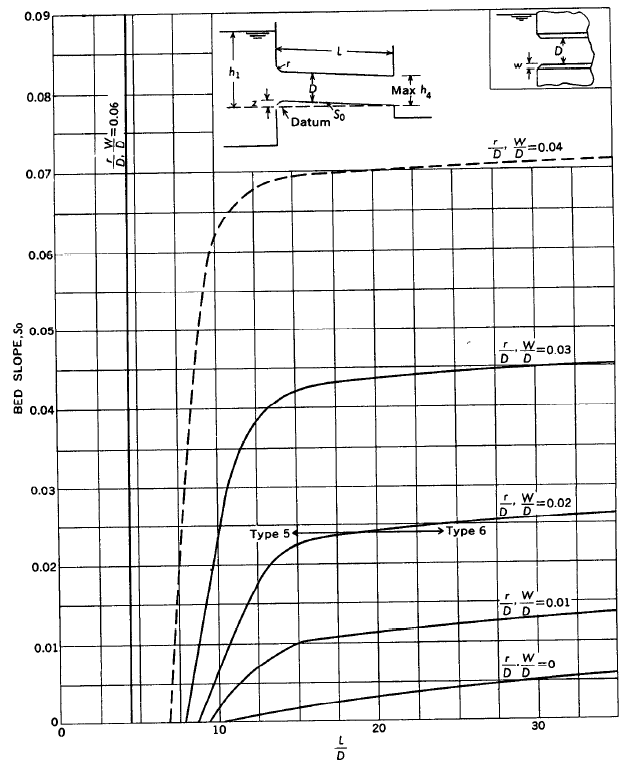
\includegraphics[width=0.6\textwidth]{graphics/culvert_fig4.png}
\end{center}
\caption{Criterion for classifying flow types 5 and 6 in concrete box or pipe culverts
with square, rounded, or bevelled entrances, either with or without wingwalls \cite{Bodhaine1968}.}
\label{fig:culvert_fig4}
\end{figure}

The head loss coefficients are subject of different studies made in laboratory experiments.
A number of authors have arrived to different values or empirical relationships for the
head loss coefficients. For instance, Bodhaine \cite{Bodhaine1968} suggests different values for
the discharge coefficient ($C_D$) for each type of flow and depending on a number of
geometric features from the culvert. The discharge coefficients can vary from 0.39 to 0.98.
Another example is Carlier \cite{Carlier1972} who proposes a non-dimensional coefficient $\mu$,
that for hydraulic structures made of only one culvert can be written as follows:
\begin{equation}
\mu = \dfrac{1}{\sqrt{C_1+C_2+C_3}}
\end{equation}
with:\\
$C_1$ the head loss coefficient at the entrance of the hydraulic structure;\\
$C_2$ the head loss coefficient in the hydraulic structure;\\
$C_3$ the head loss coefficient at the exit of the hydraulic structure.

If the general expression for the discharge $Q=\mu A \sqrt{2g\Delta H}$ proposed by
Carlier \cite{Carlier1972} is compared with the formulae given by Bodhaine \cite{Bodhaine1968},
it can be seen that the non-dimensional head loss coefficient ($\mu$),
incorporates both the effect of the discharge coefficient ($C_D$) and the continuous
and local head losses. $\Delta H$ is the head loss for each type of flow.

\subsection{Formulations for culvert simulation in TELEMAC}

TELEMAC-2D and 3D give the possibility of modelling hydraulic structures, such as bridges,
discharges under a dike or tubes in which free-surface or pressurized flows may
occur during the total simulation time.
This is done by a couple of points between which flow may occur with respect to
the water levels in the river and in the floodplain.
The subroutine BUSE is called to model this kind of structures.
Each kind of flow has its own type of discharge calculation.
The kind of formulation used to compute the flow rates can be chosen with the keyword OPTBUSE.

\subsubsection{Option 1 -- following Carlier's formulation}

With this first option, the different equations implemented to calculate the
discharges are dependent on the flow regime and follow Carlier \cite{Carlier1972}.
Then the velocities are deduced from the discharges and are taken into account as source
terms both in the continuity and momentum equations.
The critical water depth ($h_c$) is approximated to $h_c \approx 2/3 h_1$ \cite{Carlier1972}.
The figure \ref{fig:culvert_fig5} presents the different variables used to calculate the discharges.
$S_1$ and $S_2$ are the upstream and downstream water elevations, respectively, $z_1$ and $z_2$
the upstream and downstream culvert bottom elevations, $D$ the culvert height and $h_1=S_1-z_1$
and $h_2=S_2-z_2$ the upstream and downstream water depths, respectively.

\begin{figure}[H]
\begin{center}
  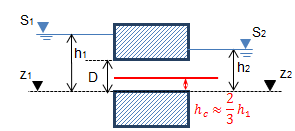
\includegraphics[width=0.5\textwidth]{graphics/culvert_fig5.png}
\end{center}
\caption{Representation of the different variables used to calculate
the discharges for each type of flow.}
\label{fig:culvert_fig5}
\end{figure}

The equations coded with this first option are described below.
Between brackets the corresponding flow type according to Bodhaine \cite{Bodhaine1968} is given.
\begin{itemize}
\item Free surface flow equations:
  \begin{itemize}
  \item Submerged weir (Bodhaine type 3)
    \begin{equation}
      Q=\mu (S_2-z_2) W \sqrt{2g(S_1-S_2 )} = (S_2-z_2) W \sqrt{\dfrac{2g(S_1-S_2)}{C_1+C_2+C_3}}
    \end{equation}
  \item Unsubmerged weir(Bodhaine type 2)
    \begin{equation}
      Q=0.385 W \sqrt{2g}(S_1-z_1)^{3/2}
    \end{equation}
  \end{itemize}
\item Pressurised flow equations:
  \begin{itemize}
  \item Submerged orifice law (Bodhaine type 4)
    \begin{equation}
      Q=\mu D W \sqrt{2g(S_1-S_2 )} = D W \sqrt{\dfrac{2g(S_1-S_2)}{C_1+C_2+C_3}}
    \end{equation}
  \item Unsubmerged orifice law
    \begin{equation}
    Q= \mu D W \sqrt{2g(S_1-S_2)} = D W \sqrt{\dfrac{2g(S_1-S_2)}{C_1+C_2}}
    \end{equation}
  \end{itemize}
\end{itemize}

The user has the possibility of assigning different values for $C_1$, $C_2$ and $C_3$.
The flow direction is imposed, \textit{e.g.}, the user can specify if the flow is going
in only one direction or in both directions and in which direction.
The keyword CLP specifies this behaviour.\\
CLP=0, flow is allowed in both directions;\\
CLP=1, flow is only allowed from section 1 to section 2\\
CLP=2, flow is only allowed from section 2 to section 1\\
CLP=3, no flow allowed.\\
A relaxation parameter ($\theta$) is introduced so that the discharge is calculated
in an explicit, implicit, or semi-implicit way.
If $\theta=1$ the calculation of the discharge is explicit while if $\theta=0$
the discharge calculation is implicit:
\begin{equation}
  Q^n=\theta Q^n + (1-\theta) Q^{n-1}
\end{equation}
Relaxation gives slower convergence speed to get the final solution
but smoothes some instabilities.
If the solution does not converge because of instabilities, the coefficient can be lowered.

\subsubsection{Option 2 -- following Bodhaine's formulation}

With this option the discharges are calculated based on the equations proposed in \cite{Bodhaine1968}
and similar to the ones incorporated in DELFT 3D model.
The flow type 1 conditions were not incorporated since they only
occur when the culvert slope is larger than the critical flow slope.
This only happens in very rare occasions if the culvert slope is very steep.
The equations used to compute the discharges are given below.\\

\underline{\textbf{Type 2 -- Critical depth at outlet}}\\
\begin{equation}
Q = \mu h_c W \sqrt{2g(S_1-(z_2+h_c))}
\end{equation}
with:
\begin{equation}
\mu = C_{D1}/\sqrt{1+\left[\dfrac{2gLn^2}{R^{4/3}} +C_v\right] C_{D1}^2 \dfrac{h_c}{h_s}^2}
\end{equation}
\begin{equation}
h_s=0.5h_c+0.5(S_1-z)
\end{equation}
\begin{equation}
R=\dfrac{h_s W}{2h_s+W}
\end{equation}

\underline{\textbf{Type 3 -- Tranquil flow}}\\
\begin{equation}
Q=\mu (S_2-z_2)W\sqrt{2g(S_1-S_2 )}
\end{equation}
with:
\begin{equation}
\mu = C_{D1}/\sqrt{ 1+\left[\dfrac{2gLn^2}{R^{4/3}} +C_v \right] C_{D1}^2 \left(\dfrac{S_2-z_2}{h_s}\right)^2}
\end{equation}
\begin{equation}
h_s=0.5(S_1-z)+0.5(S_2-z)
\end{equation}
\begin{equation}
  R=\dfrac{h_sW}{2h_s+W}
\end{equation}

\underline{\textbf{Type 4 -- Submerged outlet}}\\
\begin{equation}
Q =\mu D W \sqrt{2g(S_1-S_2)}
\end{equation}
with:
\begin{equation}
\mu = C_{D2}/\sqrt{1+\left[\dfrac{2gLn^2}{R^{4/3}} +C_v \right] C_{D2}^2}
\end{equation}
\begin{equation}
h_s=D
\end{equation}
\begin{equation}
R=\dfrac{h_s W}{2h_s+2W}
\end{equation}

\underline{\textbf{Type 5 -- Rapid flow at inlet}}\\
\begin{equation}
Q= \mu D W \sqrt{2gh_1}
\end{equation}
with:
\begin{equation}
\mu = C_{D3}
\end{equation}
\begin{equation}
h_s = D
\end{equation}
\begin{equation}
R = \dfrac{h_s W}{2h_s+2W}
\end{equation}

\underline{\textbf{Type 6 -- Full flow with free outfall}}\\
\begin{equation}
Q = \mu D W \sqrt{2g(S_1-(z_2+D))}
\end{equation}
with:
\begin{equation}
\mu = C_{D2}/\sqrt{1+\left[\dfrac{2gLn^2}{R^{4/3}} +C_v \right] C_{D2}^2}
\end{equation}
\begin{equation}
h_s=D
\end{equation}
\begin{equation}
R=\dfrac{h_s W}{2h_s+2W}
\end{equation}
The head loss coefficient expressions were obtained from experimental studies made at
Flanders Hydraulic Research.
The discharge coefficient, $C_D$, is dependent of each type of flow, being the same for
types 1, 2 and 3 ($C_{D1}$), then for types 4 and 6 ($C_{D2}$) and finally for type 5 ($C_{D3}$).
The conditions at which a certain type of flow occurs,
are presented in the table \ref{tab:culverts_tab2}.

\begin{table}[H]
\caption{Conditions for each type of flow used in TELEMAC with OPTBUSE = 2.}
\label{tab:culvert_tab2}
\begin{center}\begin{tabular}{|c|c|c|c|c|}
\hline
~ & $\mathbf{\dfrac{S_1-z_1}{D}}$ & $\mathbf{\dfrac{S_2-z_2}{D}}$ & $\mathbf{S_2-z_2}$ & $L/D$ \\
\hline
\textbf{Type 2} & $<1.5$    &  ~ & $< h_c$ & ~ \\
\hline
\textbf{Type 3} & $<1.5$    & $\le 1.0$ & $> h_c$ & ~\\
\hline
\textbf{Type 4} & $> 1.0$   & $> 1.0$ & ~ & ~\\
\hline
\textbf{Type 5} & $\ge 1.5$ & $\le 1.0$ & ~ & $< h_c$\\
\hline
\textbf{Type 6} & $\ge 1.5$ & $\le 1.0$  & ~ & $\ge h_c$\\
\hline
\end{tabular}\end{center}
\end{table}

The equations presented above are written to describe flow conditions through a
culvert system with a single pipe.
Nevertheless, additional features are sometimes incorporated in the hydraulic structures,
such as weirs in the vicinity of the culvert entrance or exit.
Such combined structures have to be taken into account.
Then the geometric features of the culvert presented in the figure \ref{fig:culvert_fig5}
are modified (see the figure \ref{fig:culvert_fig6}).
It was decided that an equivalent culvert bottom elevation should be used,
which replaces both the bottom elevations $z_1$ and $z_2$ in the formulae decribed above.
The equivalent bottom culvert elevation is then equal to the mean between $z_1$ and $z_2$.
The diameter used in the equations will be the one corresponding to the entrance of the culvert,
\textit{i.e.}, regarding the figure \ref{fig:culvert_fig6}, if the flow goes from left
to the right $D$ will be replaced by $D_1$ and on the opposite direction,
the value $D_2$ will be used.

\begin{figure}[H]
\begin{center}
  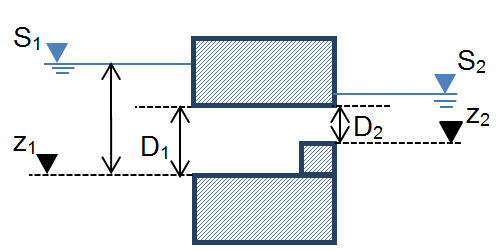
\includegraphics[width=0.5\textwidth]{graphics/culvert_fig6.png}
\end{center}
\caption{Representation of the different variables used to
calculate the discharges for each type of flow.}
\label{fig:culvert_fig6}
\end{figure}

The head loss coefficient ($\mu$ was adapted from the one calculated with the first option,
based on Carlier \cite{Carlier1972} and is used as main head loss coefficient).
Structures that caused additional head loss, like valves, grilles (trash screens) or pilars
were added in the calculation of this main coefficient.
In this way these additional features that can be present in culvert structures of
different geometric configurations are taken into account and contribute to
the flexibility of the implementation of many types of culvert structures.
The head loss due to singularities can be obtained by the general
relation \cite{Lencastre1961}, \cite{Carlier1972}:
\begin{equation}
\Delta H = C \dfrac{U^2}{2g} ~\text{or}~  U = \mu \sqrt{2g\Delta H}
\end{equation}
with:
\begin{equation}
\mu =\dfrac{1}{\sqrt{C}}
\end{equation}

The coefficient $C$ represents the sum of the different contributions for the
head loss due to singularities:
\begin{equation}
C=C_1+C_p+C_2+C_3+C_v+C_T
\end{equation}
The different contributions to this head loss coefficient $C$ will be discussed
separately and in detail here below.\\

\textbf{Coefficient} $\mathbf{C_1}$ \\
$C_1$ represents the head loss due to the contraction of the flow at the entrance
of the hydraulic structure.
Usually it is equal to 0.5 (figure \ref{fig:culvert_fig7}).
Usually, there is an abrupt contraction that will cause a head loss due to
the decelaration of the flow immediately after the culvert entrance.

\begin{figure}[H]
\begin{center}
  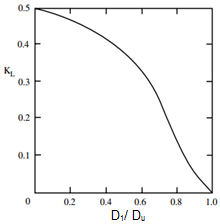
\includegraphics[width=0.5\textwidth]{graphics/culvert_fig7.png}
\end{center}
\caption{Local loss coefficient for a sudden contraction as
a function of diameter ratio between the diameter after the contraction ($D_1$)
and before the contraction $D_u$ \cite{Bruce2000}.}
\label{fig:culvert_fig7}
\end{figure}

Already in the past, Bodhaine \cite{Bodhaine1968} noticed that the discharge coefficient ($C_D$)
for type 5 flow had to be lowered comparetively with the other flow types.
It seems that the calculated discharge tends to be overestimated when the
default equation is applied. In order to take into account that effect,
a correction coefficient ($\alpha_1^5$) is applied to $C_1$ when type 5 flow occurs, such that:
\begin{equation}
\Delta H_{1.5}=\alpha_1^5 C_1  \dfrac{U^2}{2g}
\end{equation}
Comparing with the values proposed in \cite{Bodhaine1968}, $4 \le \alpha_1^5 \le 10$.\\

\textbf{Coefficient} $\mathbf{C_p}$\\
Sometimes at the entrance of culverts the flow is divided into two sections
caused by two entrance boxes instead of one but than the flow converges into
a single culvert pipe. In other words a kind of pilar is dividing the flow at the entrance.
This causes additional head loss and is taken into account.
Following Carlier \cite{Carlier1972} the head loss through parallel pillars is given by:
\begin{equation}
\Delta H_p = C_p \dfrac{U^2}{2g}
\end{equation}
where $C_p=\beta \left(Lp/b\right)^{4/3} \text{sin} \theta$  represents the head
loss coefficient due to the presence of pillars. $Lp$ is the thickness of the pillars, $b$
the free thickness between two consecutive pillars and $\beta$
a coefficient dependent on cross-shore section of the pillar.\\

\textbf{Coefficient} $\mathbf{C_2}$\\
$C_2$ represents the head loss coefficient due to the friction in the structure
and is expressed by (Lencastre, 1972):
\begin{equation}
\Delta H_2 = C_2  \dfrac{U^2}{2g} = \dfrac{2gLn^2}{R^{4/3}}\dfrac{U^2}{2g}
\end{equation}
where $L$ is the length of the structure, $n$ the Manning Strickler coefficient
of the structure and $R$ the wet cross-shore section in the structure calculated
in the code for each type of flow.
The table \ref{tab:culvert_tab3} presents the expressions for the calculation of $R$,
following what was done in the DELFT 3D model.
Here an assumption is made when calculating the hydraulic radius since the
code does not make any kind of backwater analysis to get the
precise water depths that occur in the culvert (like Mike 11 does).
\begin{table}[H]
\caption{Different parameters for each type of flow to calculate the hydraulic radius in \telemac{3d}.}
\label{tab:culvert_tab3}
\begin{center}\begin{tabular}{|c|c|c|}
\hline
\textbf{Type of flow} & $\mathbf{h_s}$ & $\mathbf{R}$ \\
\hline
\textbf{Type 2} & $0.5 h_c + 0.5(S_1-z)$    & $R = \dfrac{h_s W}{2 h_s+W}$ \\
\hline
\textbf{Type 3} & $0.5 (S_1 - z_1) + 0.5(S_2-z_2)$    & $R = \dfrac{h_s W}{2 h_s+W}$ \\
\hline
\textbf{Type 4} & $D$    & $R = \dfrac{h_s W}{2 h_s+2W}$ \\
\hline
\textbf{Type 5} & $D$    & $R = \dfrac{h_s W}{2 h_s+2W}$ \\
\hline
\textbf{Type 6} & $D$    & $R = \dfrac{h_s W}{2 h_s+2W}$ \\
\hline
\end{tabular}\end{center}
\end{table}

\textbf{Coefficient} $\mathbf{C_3}$\\
$C_3$ is the head loss coefficient due to expansion of the flow exiting the culvert.
It can be given by \cite{Lencastre1961}:
\begin{equation}
\Delta H_3 = \left(1-\dfrac{A_s}{A_{s2}}\right)^2 \dfrac{U^2}{2g} = C_3\dfrac{U^2}{2g}
\end{equation}
where $A_s$ and $A_{s2}$ are the sections in and at the downstream part of the structure.
Usually is equal to the unity for a sudden enlargement.\\

\textbf{Coefficient} $\mathbf{C_V}$\\
$C_V$ is the head loss coefficient due to the presence of a valve.
The head loss due to valves ($\Delta H_v$) can also be estimated:
\begin{equation}
\Delta H_v = C_V\dfrac{U^2}{2g}
\end{equation}
where $C_V$ depends on the type of valve and the degree of opening.
For a gate valve, some values were obtained experimentally,
and they depend on the opening of the valve \cite{Bruce2000}:
see the table \ref{tab:culvert_tab4}.
\begin{table}[H]
\caption{Values for the head loss coefficient depending on the opening of a gate valve.}
\label{tab:culvert_tab3}
\begin{center}\begin{tabular}{|c|c|}
\hline
~ & $C_V$ \\
\hline
\textbf{Wide open} & 0.2\\
\hline
\textbf{3/4 open} & 1.0 \\
\hline
\textbf{1/2 open} & 5.6 \\
\hline
\textbf{1/4 open} & 17 \\
\hline
\end{tabular}\end{center}
\end{table}

Again, a correction coefficient ($\alpha_v^5$) is applied to the head loss coefficient
due to a valve in order to take into account the increase of the head loss when type 5
flow occurs.
Through a number of laboratory experiences (IMDC Report 613\_9\_1), it can be seen that when
type 5 flow occurs, there is a greater influence of having a valve:
the associated head loss coefficient is in general much higher than for the other types of
flow (see the figure  \ref{fig:culvert_fig8}).
Please note that the variable $\alpha$ in the figure \ref{fig:culvert_fig8}
is not the same as $\alpha_v^5$.
The figure \ref{fig:culvert_fig8} is given here just to show the influence of
the valve in the different types of flow.
\begin{equation}
\Delta H_{v5} = \alpha_v^5 C_v \dfrac{U^2}{2g}
\end{equation}

\begin{figure}[H]
\begin{center}
  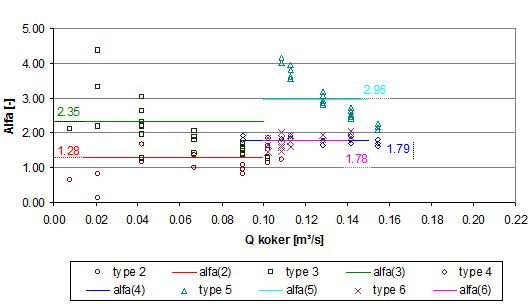
\includegraphics[width=0.95\textwidth]{graphics/culvert_fig8.png}
\end{center}
\caption{Discharge coefficient (Alfa) due to the presence of open valves for
each type of flow (source: IMDC Report 613\_9\_1)}
\label{fig:culvert_fig8}
\end{figure}

\textbf{Coefficient} $\mathbf{C_t}$\\

Trash screens are usually present at the inlet of culverts to prevent garbage
from entering or blocking the culvert. The head loss due to trash screens
($\Delta H_t$) can be estimated by its relationship with the velocity
head through the net flow area.
A number of expressions were obtained in the past by several authors.
We use the expression given by the Bureau of Reclamation \cite{Bureau1992}:
\begin{equation}
\Delta H_t = (1.45-0.45A_t-A_t^2)\dfrac{U^2}{2g} = C_t \dfrac{U^2}{2g}
\end{equation}
where $A_t=\frac{Anet}{Agross}$ gives the ratio of net flow area to gross rack area.
$U$ is the net flow velocity. The value for $C_t$ can vary between $C_t= 0$ equivalent
to not having any trash screens to approximately $C_t= 1.4$, for which the net
flow area is almost equal to the gross rack area.

Note that a very similar fomulation to this second option is included in DELFT 3D.
The main difference between the second culvert functionality in TELEMAC and the one
included in DELFT 3D is the way how the head loss coefficient is calculated.
While in TELEMAC, the Carlier reference \cite{Carlier1972} was followed, in DELFT 3D they refer
to experiments executed by Flanders Hydraulic Research.

\subsubsection{Transport of scalars through culverts}

With the implementation of the culvert functionality,
some modifications had to be done in the code such that
it would be possible to model the passage of the scalar through the culvert structure.
Following the same idea implemented to model the flow through culverts,
the concentration of the scalar in the model domain is assigned to source and sink terms
for scalars. When the flow goes from the river to the floodplain,
there is a source point in the floodplain with a scalar concentration equal to the one
in the river. At the same time in the river there is a sink term with the same scalar
concentration. The opposite happens when the flow goes from the floodplain to the river.
Please note that it is the scalar concentration that is assigned to the source term
and not the scalar concentration per second.
In its structure, TELEMAC deals with that concentration and associates it to the
discharge and volume of fluid at the source terms.
In order to take into account the transport of scalars in the model the
user has only to specify in the steering file the keywords relative to the scalars.

\subsection{Input data for \telemac{3d}}

In order to take culverts into account in \telemac{3d} the user has to define in the
steering file two keywords: \\
NUMBER OF CULVERTS \\
CULVERTS DATA FILE\\

The number of culverts has to be assigned to the keyword NUMBER OF CULVERTS
(please note that this is the number of culverts and not the number of sources/sink terms:
one culvert has two sink/source terms).
The keyword CULVERTS DATA FILE refers to an ASCII file where the geometric characteristics
and all head loss coefficients are given to be used by the code.
The text file has to follow a strict structure of the input parameters in order
for the software to read the right values for the right parameter.
Here below an example is given:\\

Relaxation, Number of culverts\\
0.05 2\\
I1  I2  CE1  CE2  CS1  CS2  LRG HAUT1 CLP LBUS Z1 Z2 CV  C56  CV5  C5 CT HAUT2 FRIC LENGTH CIRC D1  D2 A1 A2 AA\\
data culvert 1  ...\\
data culvert 2 ...\\
... \\

The index number 1 refers to the river side and the index 2 refers to the floodplain side.
I1 and I2 correspond to the index of the source/sink terms in the river side
and in the floodplain that represent the beginning and end of the culvert.
CE1, CE2 and CS1, CS2 are the head loss coefficients
for the inlet and outlet sluice entrance ($C_1$) and exit ($C_3$), respectively.
LRG represents the width of the culvert.
HAUT1 and HAUT2 the height of the culvert at the river and
floodplain side.
The flow direction is also imposed through the keyword CLP and
a relaxation parameter (variable RELAXB) is incorporated in the code.
CLP=0, flow is allowed in both directions; CLP=1, flow is only allowed from section 1 to section 2; CLP=2, flow is only allowed from section 2 to section 1; CLP=3, no flow allowed.
LBUS is the linear head loss in the culvert.
Z1 and Z2 the elevations of the culvert
extremities in the river side and in the floodplain.
CV refers to the loss coefficient due to the presence of a valve ($C_v$) and
C56 ($c$) is the constant used to differentiate flow types 5 and 6.
C5 and CV5 represent correction coefficients to C1 and to CV coefficients
due to the occurrence of the type 5 flow.
CT is the loss coefficient due to the presence of trash screens ($C_t$).
FRIC is the Manning Strikler coefficient.
The length of the culvert can be set (LENGTH parameter), and its shape can be specified through the parameter CIRC (equal to 1 in
case of a circular section, 0 for a rectangular section).
D1 and D2 are the angles that the pipe makes with respect to the bottom, in degrees.
A1 and A2 are the angles with respect to the x axis.
For a vertical intake, the angle with the bottom will therefore be 90${}^\circ$.
They are used to account for the current direction at source or sink point.
AA is a parameter which allows the user to choose whether A1 and A2 are automatically computed by TELEMAC
or whether the data file values are used to set these angles: AA=1 -- automatic angle; AA=0 -- user-set angle.
\section{\label{sec:coriolis}Coriolis%
\index{Coriolis!force}
force and centrifugal force%
\index{centrifugal force}%
}
These forces are due to the rotation of the Earth on its own axis. We
establish their expressions below. Let $\vec{k}$ be the unit vector oriented
along the rotational axis of the Earth, from South to North. The rotation
vector of the Earth can then be written as:
\begin{equation}
\vec{\Omega}=\Omega\vec{k}
\end{equation}
with $\Omega= 2\pi/T$ where $T$ is equal to $86164$: the duration in seconds of the
sidereal day.\\

Let $R_a$ be a fixed referential with its origin at the centre of the Earth and
$R_T$ a referential which turns with the Earth. In this referential, the axis $Ox$ is directed eastwards,
$Oy$ northwards and $Oz$ upwards.
For any vector $\vec{A}$, the following relation holds:
\begin{equation}
\left.\dfrac{d \vec{A}}{d t}\right|_{R_A}=\left.\dfrac{d \vec{A}}{d t}\right|_{R_T}+\vec{\Omega}\wedge\vec{A}
\end{equation}
The relation between the velocities expressed in the two referentials then reads:
\begin{equation}\label{eq:uA}
\vec{u}_{A}=\vec{u}+\vec{\Omega}\wedge\vec{r}_A
\end{equation}
which is equivalent to:%

\begin{equation}
\left(  \dfrac{d\vec{r}_A}{dt}\right)_{R_A}=\left(
\dfrac{d\vec{r}}{dt}\right)_{R_T}+\vec{\Omega
}\wedge\vec{r}_A%
\end{equation}


%This relation is a rule for time derivatives, valid for every vector with
%components in referentials $a$ and $b$. In fact, for every vector
%$\vec{i}$ of the spinning referential, $b$, we have:
%\[
%\dfrac{d\vec{i}}{dt}=\vec{\omega}\wedge\vec{i}%
%\]
By deriving $\vec{u}_{A}$ with respect to time, we get:%

\begin{equation}
\begin{array}{ll}
\left(  \dfrac{d\vec{u}_{A}}{dt}\right)_{R_A}&=\left(
\dfrac{d\vec{u}_A}{dt}\right)  _{R_T}%
+\vec{\Omega}\wedge\vec{u}_A\smallskip\\
&=\left(
\dfrac{d\vec{u}}{dt}\right)_{R_T}
+\left(\dfrac{d\vec{\Omega}}{dt}\right)_{R_T}\wedge\vec{r}
+\vec{\Omega}\wedge\left(  \dfrac
{d\vec{r}}{dt}\right)_{R_T}
+\vec{\Omega}\wedge\vec{u}
+\vec{\Omega}\wedge(\vec{\Omega}\wedge\vec{r})
\end{array}
\end{equation}
The second line is obtained by replacing $\vec{u}_A$ with its expression \eqref{eq:uA} in the first line.
The term $\left(d\vec{\Omega}/dt\right)_{R_T}$ is equal to 0 and $\left(d\vec{r}/dt\right)_{R_T}$
is equal to $\vec{u}$ by definition. We then have:
\begin{equation}
\left(  \dfrac{d\vec{u}_{A}}{dt}\right)_{R_A}=
\left(\dfrac{d\vec{u}}{dt}\right)_{R_T}
+2\vec{\Omega}\wedge\vec{u}
+\vec{\Omega}\wedge(\vec{\Omega}\wedge\vec{r})
\end{equation}
The last term of this equation is oriented along the vertical.
To write the equations of motion in the referential linked to the surface of the Earth,
it is then necessary to include the terms:
\begin{equation}
-2\,\vec{\Omega}\wedge\vec{u}%
\end{equation}
which is called the Coriolis force, as well as:
\begin{equation}
-\vec{\Omega}\wedge(\vec{\Omega}\wedge\vec{r})
\end{equation}
which is called the centrifugal force.

In the referential linked to the surface of the Earth, the vector $\vec{\Omega}$ reads:%

\begin{equation}
\vec{\Omega}=\left(
\begin{array}
[c]{c}%
\Omega_{x}\\
\Omega_{y}\\
\Omega_{z}%
\end{array}
\right)  =\left(
\begin{array}
[c]{c}%
0\\
\Omega\cos(\lambda)\\
\Omega\sin(\lambda)
\end{array}
\right)
\end{equation}
where $\lambda$ is the latitude at the considered point, counted positively
from the equator to the North pole and negatively from the equator to the South pole.
%In the more general case where north makes an angle $N$ with the axis $Oy$
%(counted positively on going from $Oy$ to the north), one has:
%\begin{equation}
%\vec{\Omega}=\left(
%\begin{array}
%[c]{c}%
%\Omega_{x}\\
%\Omega_{y}\\
%\Omega_{z}%
%\end{array}
%\right)  =\left(
%\begin{array}
%[c]{c}%
%\Omega\cos(\lambda)\sin(N)\\
%\Omega\cos(\lambda)\cos(N)\\
%\Omega\sin(\lambda)
%\end{array}
%\right)
%\end{equation}
The Coriolis force then reads:
\begin{equation}\label{eq:coriolis_complet}
-2\vec{\Omega}\wedge\vec{u}=-2\Omega\left(
\begin{array}
[c]{c}%
\cos(\lambda)w-\sin(\lambda)v\\
\sin(\lambda)u\\
\cos(\lambda)u
\end{array}
\right)
\end{equation}
The Coriolis force only has an effect on large scale flows, and is thus
usually considered in the frame of quasi-horizontal flows.
In this context, the vertical velocities are neglected. Besides,
the effect of the Coriolis force along the vertical are not taken into account
since they are negligible compared to the gravity term.
Thus, the equation \eqref{eq:coriolis_complet} becomes:
\begin{equation}\label{eq:coriolis_complet}
-2\,\vec{\Omega}\wedge\vec{u}=-2\Omega\left(
\begin{array}
[c]{c}%
-\sin(\lambda)v\\
\sin(\lambda)u\\
0
\end{array}
\right)
\end{equation}

By definition, the Coriolis coefficient%
\index{Coriolis!coefficient}
is defined by:
\begin{equation}
\gamma=2\Omega\sin(\lambda)
\end{equation}
It is about equal to $10^{-4}s^{-1}$ at
a latitude of 45$^\circ$N. The Coriolis forces have a significant impact on the
fluid motion when their magnitude is of the same order as the inertia forces.
This is measured by the Rossby number, that corresponds to the ratio between
inertia and Coriolis forces:
\begin{equation}
R_{0}=\dfrac{U}{\gamma L}%
\end{equation}
where $U$ and $L$ are characteristic horizontal velocity and length of flow. The
Coriolis force has a significant impact when $R_{0}\ge 1$; that is, for large oceanic or
atmospheric areas: for example, considering an oceanic flow with characteristic
horizontal velocity 1 m s$^{-1}$ and $\gamma$ equal to 10$^{-4}$, the Coriolis force
becomes significant for horizontal length scales larger than 10 km.
It is however negligible in rivers and lakes (and even more so in kitchen sinks...).

\begin{CommentBlock}{Remark:}
The term due to the vertical
velocity is ignored in \telemac{3d}; however, it may have some importance
in oceanic flows on the mesoscale, as pointed out by Mahadevan \textit{et al.} \cite{mahadevan96}.
\end{CommentBlock}

For a geophysical flow, the centrifugal force is not added to the
Navier--Stokes equations. In fact, one considers that the free surface of a
fluid at rest coincides with an equipotential surface of apparent gravity,
which already integrates the effect of centrifugal force.

% ---------------------------------------------------------------------------
\section{Arbitrary Lagrangian-Eulerian formulation}\label{sec:ALE}
% ---------------------------------------------------------------------------

\subsection{Principle}
The Arbitrary Lagrangian-Eulerian (ALE) formulation was developed in order to
simplify the treatment of problems with moving boundaries, in particular
for fluid-structure interaction problems and for flows with moving interfaces
(see \cite{Hirt1974, Chan1975, Donea1981}, for example). It is reviewed and interpreted
in a Finite Elements context, with a view of using it in \telemac{3d}, in \cite{Decoene2006}.
In \cite{Decoene2009}, Decoene \textit{et al.} demonstrated the equivalence between the
ALE formulation and the classical sigma-transform with a particular type of ALE mapping.
They introduced a generalised form of the sigma transformation, which can now be used in
\telemac{3d}.

The idea of the ALE formulation is to define a reference configuration -- generally chosen
to be fixed, and a mapping that gives the correspondence between the real domain and
the reference domain. The mapping can be arbitrarily chosen, but it has to
be conforming to the evolution of the domain boundaries.

The idea is then to compute the time-derivatives in the reference domain,
which is simpler than in the real (moving) domain. Indeed, in the moving domain,
the discretisation of a time derivative of a field $\vec{u}$ at position $\vec{x}$ cannot be written as:
\begin{equation}
\dfrac{\partial \vec{u}}{\partial t}(\vec{x},t) \approx \dfrac{\vec{u}(\vec{x},t^{n+1})-\vec{u}(\vec{x},t^n)}{\delta t}
\end{equation}
since $\vec{x}$ may not be in the computational domain anymore at time $t^{n+1}$.\\

Throughout this document, the reference mesh is denoted by $\Omega^*$, and
the fields in the reference mesh are denoted with a $*$ superscript.
We denote by $\mathcal{A}^*$ the mapping that associates to each point $\vec{x}^*$ in $\Omega^*$ a
point $\vec{x}$ in $\Omega$, and $\mathcal{A}$ the mapping that associates to each point $\vec{x}$ in $\Omega$ a
point $\vec{x}^*$ in $\Omega^*$. Here, we dropped the time-dependence
in the notations to simplify, but keep in mind that $\Omega$ varies in time, as well as $\mathcal{A}^*$.
$\vec{x}^*$ represents the coordinates in the reference domain.
It is assumed in \telemac{3d} that $\mathcal{A}^*$ is invertible with continuous inverse $\mathcal{A}$.

\begin{WarningBlock}{Warning:}
Note that this assumption makes it impossible for \telemac{3d} to treat the breaking
of the free-surface based on this ALE formulation.
\end{WarningBlock}

The time-derivative of a field $f$ in the reference domain is
denoted by $\left(\partial f/\partial t\right)_{x^*,y^*,z^*}(\vec{x},t)$.
In \telemac{3d} the mesh motion is only allowed along the vertical and in the
reference mesh, only the $z$ coordinate is modified.
The other coordinates and time remain unchanged. In other words, $t^{\ast}=t
$, $x^{\ast}=x$ and $y^{\ast}=y$.
The instantaneous domain velocity is defined by:
\begin{equation}\label{c_def}
\vec{c}(x,y,z^*,t)=\dfrac{\partial \mathcal{A}^*}{\partial t}
\end{equation}
Considering that, by definition of the mapping, $\vec{x}=\mathcal{A}^*(\vec{x}^*)$,
the domain velocity can also be written as follows:
\begin{equation}
\vec{c}(x,y,z^*,t)=\left(\dfrac{\partial \vec{x}}{\partial t}\right)_{x,y,z^*}=\left(\dfrac{\partial z}{\partial t}\right)_{x,y,z^*}\vec{e}_z=\left(0, 0, c\right)
\end{equation}
The Jacobian matrix of $\mathcal{A}^*$ is denoted by $\vec{J}^*$ and defined by:
\begin{equation}
J_{ij}^*(x,y,z^*,t)=\dfrac{\partial \mathcal{A}^*(x^*_i)}{\partial x^*_j}
\end{equation}
The continuous expression of the Jacobian
determinant is then:
\begin{equation}
J^*(x,y,z^*,t)=\left(\dfrac{\partial z}{\partial z^*}\right)_{x,y,t}
\end{equation}

In \telemac{3d}, the domain motion is managed through the sigma transformation,
either in its classical or its generalised form.
It is necessary here to introduce one notion of the space discretisation in
\telemac{3d}, which is that the mesh is structured on the vertical.
It is built as an extrusion of a 2D mesh along the vertical, then divided into layers.
A transformation of the variable $z$ is then done for each layer,
so that $z^*$ is equal to $0$ at the bottom of a layer and $1$ at the top.
With the generalised sigma transform, the change of variable consists in defining $z^*$ as:
\begin{align}
z^* =& \dfrac{z-z_{ip}}{z_{ip+1}-z_{ip}} = \dfrac{z-z_{ip}}{\Delta z}
\end{align}
where $z_{ip}$ is the elevation of the bottom of layer $p$ at point $i$,
$z_{ip+1}$ is the elevation of the top of layer $p$ at point $i$ and $\Delta z$ is the height of the layer $p$,
which is piecewise constant vertically.

\begin{CommentBlock}{Classical version of the sigma transformation:}
The classical sigma transformation consists in changing the vertical
coordinates so that the bed elevation becomes 0 and the free surface
elevation becomes 1. The following change of variables is then used:%
\begin{equation}
z^{\ast}=\dfrac{z-b}{\eta-b}=\dfrac{z-b}{h}%
\end{equation}
This is an affine transformation giving a transformed domain $\Omega^{*} $.
The elevations are shifted and multiplied by a coefficient $1/h$. For a
function $f$, the volume integrals are thus modified in the following manner:%
\begin{equation}
\int_{\Omega} f~d\Omega = \int_{\Omega^{\ast}}\left(\dfrac{\partial z}{\partial z^{\ast}}\right)_{x,y,t}
f^{\ast}~d\Omega^{\ast}=\int_{\Omega^{\ast}}h f^\ast ~d\Omega^{\ast}
\end{equation}
\end{CommentBlock}

From now on we shall denote the Jacobian by $\Delta z$:
\begin{equation}
J^*=\left(\dfrac{\partial z}{\partial z^{\ast}}\right)_{x,y,t}=\Delta z
\end{equation}
As a matter of fact, it will appear in the section \ref{transformation sigma}, when we deal
with the generalized sigma transformation on 3D meshes, that the Jacobian is the
local height of prisms, the depth $h$ being then the sum of these heights along the vertical.

\subsection{Writing the Navier--Stokes equations in the reference domain}
\paragraph{Space and time derivatives:}
To change referentials it is necessary to express the derivatives in the reference domain
as functions of the derivatives in the real domain.
Be careful that a partial derivative with respect to $x$ in the reference domain
implies that one derives with constant $y$, $z^{\ast}$ and $t$.
In what follows the subscripts indicate what variables remain constant in the derivation.
Then, $(\partial f/\partial x)_{y,z^*,t}$ and $(\partial f/\partial x)_{y,z,t}$ do not have the same meaning.
For space derivatives, we shall use the following basic relations:%
\begin{equation}
\left(  \dfrac{\partial f}{\partial x}\right)  _{y,z,t}\,=\,\left(
\dfrac{\partial f}{\partial x}\right)  _{y,z^{\ast},t}\,+\,\,\,\left(
\dfrac{\partial f}{\partial z^{\ast}}\right)  _{x,y,t}\,\,\left(
\dfrac{\partial z^{\ast}}{\partial x}\right)  _{y,z,t}\, \label{transfsig}%
\end{equation}
%
\begin{equation}
\left(  \dfrac{\partial f}{\partial y}\right)  _{x,z,t\,}\,=\,\left(
\dfrac{\partial f}{\partial y}\right)  _{x,z^{\ast},t\,}\,+\,\,\,\left(
\dfrac{\partial f}{\partial z^{\ast}}\right)  _{x,y,t}\,\,\left(
\dfrac{\partial z^{\ast}}{\partial y}\right)  _{x,z,t\,} \label{transfsig3}%
\end{equation}
%
\begin{equation}
\left(  \dfrac{\partial f}{\partial z}\right)  _{x,y,t\,}\,=\,\,\,\,\left(
\dfrac{\partial f}{\partial z^{\ast}}\right)  _{x,y,t\,}\,\,\left(
\dfrac{\partial z^{\ast}}{\partial z}\right)  _{x,y,t\,} \label{transfsig4}%
\end{equation}

\begin{CommentBlock}{Demonstration of the relation \eqref{transfsig}:}
\begin{align*}
\left(\dfrac{\partial f}{\partial x}\right)_{y,z,t} = &
	\left(\dfrac{\partial f}{\partial x^*}\right)_{y,z^*,t} \left(\dfrac{\partial x^*}{\partial x}\right)_{y,z,t}
	+\left(\dfrac{\partial f}{\partial y^*}\right)_{x,z^*,t} \left(\dfrac{\partial y^*}{\partial x}\right)_{y,z,t}
	+\left(\dfrac{\partial f}{\partial z^*}\right)_{x,y,t}\left(\dfrac{\partial z^*}{\partial x}\right)_{y,z,t}
\end{align*}
Since $x^* = x$ and $y^* = y$, $\left(\partial x^*/\partial x\right)_{y,z,t}=1$
and  $\left(\partial y^*/\partial x\right)_{y,z,t}=0$. Equation \eqref{transfsig} is thus obtained.
The equations \eqref{transfsig3} and \eqref{transfsig4} are obtained in the same way.
\end{CommentBlock}

Regarding the time-derivatives, the following basic formula will be used:
\begin{equation}
\left(  \dfrac{\partial f}{\partial t}\right)_{x,y,z\,}=\left(
\dfrac{\partial f}{\partial t}\right)_{x,y,z^{\ast}}+\left(
\dfrac{\partial f}{\partial z^{\ast}}\right)_{x,y,t}\left(
\dfrac{\partial z^{\ast}}{\partial t}\right)_{x,y,z} \label{transfsig2}%
\end{equation}

\begin{CommentBlock}{Remark:}
The equation \eqref{transfsig2} is equivalent to:
\begin{equation}\label{transfsig2bis}
\left(\dfrac{\partial f}{\partial t}\right)_{x,y,z^*}=\left(\dfrac{\partial f}{\partial t}\right)_{x,y,z}
+\vec{c} \cdot \Grad f
\end{equation}
which is a more  classical way to write this transport equation.
\end{CommentBlock}


By taking $f=z$ in the equations \eqref{transfsig} to \eqref{transfsig2},
and using our notation for the Jacobian, this
gives properties that will be used to write the Navier -- Stokes equations
in the reference domain:

\begin{equation}
\left(\dfrac{\partial z^{\ast}}{\partial x}\right)_{y,z,t}
=-\dfrac{1}{\Delta z}\left(\dfrac{\partial z}{\partial x}\right)
_{y,z^{\ast},t} \label{form1}%
\end{equation}
%
\begin{equation}
\left(\dfrac{\partial z^{\ast}}{\partial y}\right)_{x,z,t}
=-\dfrac{1}{\Delta z}\left(\dfrac{\partial z}{\partial y}\right)
_{x,z^{\ast},t} \label{form2}%
\end{equation}
%
\begin{equation}
\left(\dfrac{\partial z^{\ast}}{\partial t}\right)_{x,y,z}
=-\dfrac{1}{\Delta z}\left(\dfrac{\partial z}{\partial t}\right)
_{x,y,z^{\ast}} \label{form3}%
\end{equation}

Let $\vec{c}^*$ be defined by:
\begin{equation}\label{c*_def}
\vec{c}^*=\left(\dfrac{\partial z^*}{\partial t}\right)_{x,y,z}=\left(0, 0, c^*\right)
\end{equation}
$\vec{c}^*$ can be interpreted as the velocity of the reference domain.
With the definition of the domain's velocity given by \eqref{c_def}, the equation
\eqref{form3} reads:
\begin{equation}\label{velocitiesmesh}
\vec{c}+\Delta z\vec{c}^*=0
\end{equation}

The following equality holds:
\begin{equation}
\dfrac{\partial}{\partial t}\left(  \dfrac{\partial z}{\partial z^{\ast}%
}\right)_{x,y,t} = \dfrac{\partial}{\partial z^{\ast}}\left(  \dfrac{\partial
z}{\partial t}\right)_{x,y,z^*}
\end{equation}
which reads, with our notations:
\begin{equation}
\dfrac{\partial \Delta z}{\partial t} - \dfrac{\partial c_z}{\partial z^{\ast}}
= \dfrac{\partial \Delta z}{\partial t} - \Divast \vec{c} = 0
\end{equation}
Using the equation \eqref{velocitiesmesh} to replace $\vec{c}$ in the previous relation, it is equivalent to:
\begin{equation}
\dfrac{\partial \Delta z}{\partial t}+\Divast(\Delta z\vec{c}^*)=0
\end{equation}
%Using equation \eqref{velocitiesmesh} to replace $\vec{c}^*$ in the previous relation, we get:
%\begin{equation}
%\dfrac{\partial}{\partial t}\left(\dfrac{1}{\Delta z}\right)+\dfrac{\partial}{\partial
%z^{\ast}}\left(\dfrac{\vec{c}}{\Delta z}\right)=\dfrac{\partial}{\partial t}\left(\dfrac{1}{\Delta z}\right)+\Div\left(\dfrac{\vec{c}}{\Delta z}\right)=0
%\end{equation}
In the same way, we find:
\begin{equation}
\dfrac{\partial}{\partial t}\left(\dfrac{1}{\Delta z}\right)+\dfrac{\partial}{\partial
z^{\ast}}\left(\dfrac{\vec{c}}{\Delta z}\right)=\dfrac{\partial}{\partial t}\left(\dfrac{1}{\Delta z}\right)+\Div\left(\dfrac{\vec{c}}{\Delta z}\right)=0
\end{equation}

This can be interpreted as an evolution law for the Jacobian determinant.
It ensures the conservation of the domain's volume when changing referentials and will have
to be fulfilled in the discrete framework.
%With this formula and using the equation \eqref{transfsig2bis}, the following relation is obtained:
%\begin{equation}
%\dfrac{d}{dt}\int_\Omega f(\vec{x},t)~d\Omega = \int_\Omega
%\left[\left(\dfrac{\partial f}{\partial t}\right)_{x,y,z^*}+f(\vec{x},t)\Div \vec{c}\right]~d\Omega
%\end{equation}

%$\overrightarrow{W}_{mesh}$ will be the vector with components (0,0,$W_{mesh}
%$). We shall also encounter in the derivations a quantity which can be
%interpreted as the velocity of the transformed mesh:%
%
%\begin{equation}
%W_{mesh}^{\ast}=\left(  \dfrac{\partial z^{\ast}}{\partial t}\right)  _{x,y,z}%
%\end{equation}
%
%
%Equation \eqref{form3} is thus also:%
%
%\begin{equation}
%W_{mesh}+\Delta zW_{mesh}^{\ast}=0 \label{velocitiesmesh}%
%\end{equation}
%and the fact that we have:%
%
%\[
%\dfrac{\partial}{\partial t}\left(  \dfrac{\partial z}{\partial z^{\ast}%
%}\right)  -\dfrac{\partial}{\partial z^{\ast}}\left(  \dfrac{\partial
%z}{\partial t}\right)  =0
%\]
%leads to:%
%
%\[
%\dfrac{\partial(\Delta z)}{\partial t}-\dfrac{\partial(W_{mesh})}{\partial
%z^{\ast}}=\dfrac{\partial(\Delta z)}{\partial t}-div^{\ast}(\overrightarrow{W}%
%_{mesh})=0
%\]
%or:%
%
%\begin{equation}
%\dfrac{\partial(\Delta z)}{\partial t}+div^{\ast}(\Delta z\overrightarrow{W}%
%_{mesh}^{\ast})=0
%\end{equation}
%
%
%In the same way we find:%
%
%\begin{equation}
%\dfrac{\partial(\dfrac{1}{\Delta z})}{\partial t}+div\left(  \dfrac
%{\overrightarrow{W}_{mesh}}{\Delta z}\right)  =0
%\end{equation}


\paragraph{Advection terms:%
\index{advection}%
}

The advection terms must be carefully examined in a moving grid because the
advected functions vary not only under the effect of the flow, but also
because they are defined on moving points. The derivative $df/dt$,
written in the real domain, reads:%
\begin{equation}
\dfrac{df}{dt}=\dfrac{\partial f}{\partial t}
+u\dfrac{\partial f}{\partial x}
+v\dfrac{\partial f}{\partial y}
+w\dfrac{\partial f}{\partial z} \label{ugrad}%
\end{equation}
From now on, for the sake of simplicity, we drop the subscripts when the derivatives are estimated in the real domain.
Using the formula \eqref{transfsig}, this equation becomes:
\begin{equation}\label{formulaTimeDeriv}
\begin{array}{lll}
\dfrac{df}{dt} & = \dfrac{\partial f}{\partial t}
+u\left(\dfrac{\partial f}{\partial x}\right)_{y,z^*,t}
+u\dfrac{\partial f}{\partial z^{\ast}}\dfrac{\partial z^{\ast}}{\partial x}
+v\left(\dfrac{\partial f}{\partial y}\right)_{x,z^*,t}
+v\dfrac{\partial f}{\partial z^{\ast}}\dfrac{\partial z^{\ast}}{\partial y}
+w\dfrac{\partial f}{\partial z^{\ast}}\dfrac{\partial z^{\ast}}{\partial z}\bigskip\\
&=\dfrac{\partial f}{\partial t}+u\left(\dfrac{\partial f}{\partial x}\right)_{y,z^*,t}
+v\left(\dfrac{\partial f}{\partial y}\right)_{x,z^*,t}
+\left(u\dfrac{\partial z^{\ast}}{\partial x}
+v\dfrac{\partial z^{\ast}}{\partial y}
+w\dfrac{\partial z^{\ast}}{\partial z}\right)\dfrac{\partial f}{\partial z^{\ast}}
\end{array}
\end{equation}

%\begin{equation}
%\dfrac{df}{dt}=\left(\dfrac{\partial f}{\partial t}\right)_{x,y,z}%
%+u\left(\dfrac{\partial f}{\partial x}\right)_{y,z^*,t}
%+v\left(\dfrac{\partial f}{\partial y}\right)_{x,z^*,t}
%+\left(u\left(\dfrac{\partial z^{\ast}}{\partial x}\right)_{y,z,t}
%+v\left(\dfrac{\partial z^{\ast}}{\partial y}\right)_{x,z,t}
%+w\left(\dfrac{\partial z^{\ast}}{\partial z}\right)_{x,y,t}\right)\left(\dfrac{\partial f}{\partial z^{\ast}}\right)_{x,y,t}
%\end{equation}

On the other hand, the velocities in the transformed mesh are defined by:
\begin{equation}
u_{\ast}=\dfrac{dx^{\ast}}{dt}=\dfrac{dx}{dt}=u
\end{equation}
%
\begin{equation}
v^{\ast}=\dfrac{dy^{\ast}}{dt}=\dfrac{dy}{dt}=v
\end{equation}
%
\begin{equation}
w^{\ast}=\dfrac{dz^{\ast}}{dt}%
\end{equation}
The vertical velocity in the transformed mesh, $w^*$, is also equal to:%
\begin{equation}
w^{\ast}=\dfrac{\partial z^{\ast}}{\partial t}
+u\dfrac{\partial z^{\ast}}{\partial x}
+v\dfrac{\partial z^{\ast}}{\partial y}
+w\dfrac{\partial z^{\ast}}{\partial z} \label{wetoile}%
\end{equation}
The equation \eqref{formulaTimeDeriv} thus becomes:%
\begin{equation}
\dfrac{df}{dt}=\dfrac{\partial f}{\partial t}
+u\left(\dfrac{\partial f}{\partial x}\right)_{y,z^*,t}
+v\left(\dfrac{\partial f}{\partial y}\right)_{x,z^*,t}
+(w^{\ast}-c^{\ast})\dfrac{\partial f}{\partial z^{\ast}}
\label{gradstar}%
\end{equation}
When the mesh is moving, $f^{n+1}$ and $f^{n}$ correspond to points having the same $x$, $y $
and $z^{\ast}$, but not the same $z$. The partial derivatives in time in our
equations are thus expressed using $\left(\partial f/\partial t\right)_{x,y,z^{\ast}}$.
Using the equation \eqref{transfsig2}, the equation \eqref{gradstar} then becomes:%
\begin{equation}
\dfrac{df}{dt}=\left(\dfrac{\partial f}{\partial t}\right)_{x,y,z^{\ast}}
+u\left(\dfrac{\partial f}{\partial x}\right)_{y,z^*,t}
+v\left(\dfrac{\partial f}{\partial y}\right)_{x,z^*,t}
+w^{\ast}\dfrac{\partial f}{\partial z^{\ast}}
\end{equation}

Advection equations, in the transformed mesh and taking into account the
motion of the real mesh, will then have the simple form:%
\begin{equation}
\left(\dfrac{\partial f}{\partial t}\right)_{x,y,z^{\ast}}
+u\left(\dfrac{\partial f}{\partial x}\right)_{y,z^*,t}
+v\left(\dfrac{\partial f}{\partial y}\right)_{x,z^*,t}
+w^{\ast}\dfrac{\partial f}{\partial z^{\ast}}=0 \label{advectioninfixedmesh}%
\end{equation}

\begin{CommentBlock}{Equivalence between the sigma transformation and the ALE formulation}
Comparing the equations \eqref{gradstar} and \eqref{ugrad} shows that:%
\begin{equation}
u\dfrac{\partial f}{\partial x}
+v\dfrac{\partial f}{\partial y}
+w\dfrac{\partial f}{\partial z}
= u\left(\dfrac{\partial f}{\partial x}\right)_{y,z^*,t}
+v\left(\dfrac{\partial f}{\partial y}\right)_{x,z^*,t}
+(w^{\ast}-c^{\ast})\dfrac{\partial f}{\partial z^{\ast}}
\end{equation}
while the equation \eqref{velocitiesmesh}, combined with \eqref{transfsig} and \eqref{wetoile}, also yields:%
\begin{equation}
u\dfrac{\partial f}{\partial x}
+v\dfrac{\partial f}{\partial y}
+(w-c)\dfrac{\partial f}{\partial z}
=u\left(\dfrac{\partial f}{\partial x}\right)_{y,z^*,t}
+v\left(\dfrac{\partial f}{\partial y}\right)_{x,z^*,t}
+w^{\ast}\dfrac{\partial f}{\partial z^{\ast}}
\end{equation}
This shows that using the sigma transformation is equivalent to writing the equations in the ALE framework
at the continuous level. In the section \ref{sec:FS-NS}, the Navier--Stokes
equations will thus be written in the ALE framework,
using $\vec{u}-\vec{c}$ instead of $\vec{u}$ for the advection terms.
\end{CommentBlock}

\paragraph{Divergence:%
\index{divergence}%
}

We now want to write $\Div \vec{u}$ in the transformed mesh. Using
the formula \eqref{transfsig}, we have:%
\begin{equation}
\Div\vec{u}=\left(\dfrac{\partial u}{\partial x}\right)_{y,z\ast,t}
+\dfrac{\partial u}{\partial z^{\ast}}\dfrac{\partial z^{\ast}}{\partial x}
+\left(\dfrac{\partial v}{\partial y}\right)_{x,z^{\ast},t}
+\dfrac{\partial v}{\partial z^{\ast}}\dfrac{\partial z^{\ast}}{\partial x}
+\dfrac{\partial w}{\partial z^{\ast}}\dfrac{\partial z^{\ast}}{\partial z}
\end{equation}

By multiplying the previous equation by $\Delta z=(\partial z/\partial z^{\ast})_{x,y,t}$,
which depends on $x$, $y$ and $t$, but not on $z$ or $z^{\ast}$, and using the fact that:
\begin{equation}
\Delta z\left(  \dfrac{\partial u}{\partial x}\right)_{y,z^{\ast},t}=\left(
\dfrac{\partial \Delta z u}{\partial x}\right)_{y,z^{\ast},t}-u\dfrac{\partial \Delta z}{\partial x}
\end{equation}
we then get:%
\begin{equation}
\begin{array}{ll}
\Delta z\Div\vec{u} & =\left(\dfrac{\partial \Delta z u}{\partial
x}\right)_{y,z^{\ast},t}-u\dfrac{\partial \Delta z}{\partial x}+
\dfrac{\partial \Delta zu}{\partial z^{\ast}}\dfrac{\partial z^{\ast}}{\partial x}
+\left(\dfrac{\partial \Delta zv}{\partial y}\right)_{x,z^{\ast},t}\medskip \\
& -v\dfrac{\partial \Delta z}{\partial y}+
\dfrac{\partial \Delta z v}{\partial z^{\ast}}\dfrac{\partial z^{\ast}}{\partial y}
+\dfrac{\partial \Delta zw}{\partial z^{\ast}}\dfrac{\partial z^{\ast}}{\partial z} \label{toto}%
\end{array}
\end{equation}


The term $\partial \Delta zw^{\ast}/\partial z^{\ast}$ can be calculated using
the equation \eqref{wetoile}:%
\begin{equation}
\begin{array}{ll}
 \dfrac{\partial \Delta zw^{\ast}}{\partial z^{\ast}}&=
\dfrac{\partial}{\partial z^{\ast}}\left(  \Delta z\dfrac{\partial
z^{\ast}}{\partial t}\,+ \Delta zu\dfrac{\partial z^{\ast}}{\partial x}+\Delta z
v\dfrac{\partial z^{\ast}}{\partial y}+ \Delta zw\dfrac{\partial z^{\ast}%
}{\partial z}\right)\bigskip\\
&= \dfrac{\partial \Delta zu}{\partial z^{\ast}}
\dfrac{\partial z^{\ast}}{\partial x}+\dfrac{\partial \Delta zv}{\partial
z^{\ast}}\dfrac{\partial z^{\ast}}{\partial y}+
\dfrac{\partial \Delta zw}{\partial z^{\ast}}\dfrac{\partial
z^{\ast}}{\partial z}\bigskip\\
&+\Delta z\dfrac{\partial}{\partial z^{\ast}}\left(  \dfrac{\partial z^{\ast}%
}{\partial t}\right)  + \Delta zu\dfrac{\partial}{\partial z^{\ast}}\left(
\dfrac{\partial z^{\ast}}{\partial x}\right)  + \Delta zv\dfrac{\partial
}{\partial z^{\ast}}\left(  \dfrac{\partial z^{\ast}}{\partial y}\right)
+\Delta zw\dfrac{\partial}{\partial z^{\ast}}\left(  \dfrac{\partial z^{\ast}%
}{\partial z}\right)
\end{array}
\end{equation}

The equations \eqref{form1} to \eqref{form3} give:%

\begin{equation}
\dfrac{\partial}{\partial z^{\ast}}\left(  \dfrac{\partial z^{\ast}}{\partial
t}\right)  _{x,y,z}=-\dfrac{1}{\Delta z}\dfrac{\partial \Delta z}{\partial t}%
\end{equation}
%

\begin{equation}
\dfrac{\partial}{\partial z^{\ast}}\left(  \dfrac{\partial z^{\ast}}{\partial
x}\right)  _{y,z,t}=-\dfrac{1}{\Delta z}\dfrac{\partial \Delta z}{\partial x}%
\end{equation}
%

\begin{equation}
\dfrac{\partial}{\partial z^{\ast}}\left(  \dfrac{\partial z^{\ast}}{\partial
y}\right)  _{x,z,t}=-\dfrac{1}{\Delta z}\dfrac{\partial \Delta z}{\partial y}%
\end{equation}


We now assume that the Jacobian%
\index{Jacobian}
$\Delta z$ is constant vertically (which will be our case on every finite
element), and we thus have:%

\begin{equation}
\dfrac{\partial}{\partial z^{\ast}}\left(  \dfrac{\partial z^{\ast}}{\partial
z}\right)  _{x,y,t}=0
\end{equation}

\begin{WarningBlock}{Warning:}
Here the assumption of a constant Jacobian along the vertical (it will actually be constant per layer)
is strong and prevents us from using quadratic elements along the vertical of the domain.
To use such elements, it would be necessary to properly write the corresponding equation
on $(\Delta z~\Div\vec{u})$ in the reference mesh.
\end{WarningBlock}

All this leads to:%

\begin{equation}
\begin{array}{ll}
\dfrac{\partial \Delta zw^{\ast}}{\partial z^{\ast}}&=
\dfrac{\partial \Delta zu}{\partial z^{\ast}}
\dfrac{\partial z^{\ast}}{\partial x}+\dfrac{\partial\Delta
zv}{\partial z^{\ast}}\dfrac{\partial z^{\ast}}{\partial
y}+\dfrac{\partial \Delta zw}{\partial z^{\ast}}
\dfrac{\partial z^{\ast}}{\partial z}\medskip \\
&-\dfrac{\partial \Delta z}{\partial t}-u\dfrac{\partial \Delta z}{\partial
x}-v\dfrac{\partial \Delta z}{\partial y}%
\end{array}
\end{equation}
We deduce from this that:
\begin{equation}
\begin{array}{ll}
\dfrac{\partial \Delta zw}{\partial z^{\ast}}
\dfrac{\partial z^{\ast}}{\partial z}&=\dfrac{\partial \Delta zw^{\ast}%
}{\partial z^{\ast}}+\dfrac{\partial \Delta z}{\partial
t}+u\dfrac{\partial \Delta z}{\partial x}+v\dfrac{\partial \Delta z}{\partial y}\medskip \\
&-\dfrac{\partial \Delta zu}{\partial z^{\ast}}
\dfrac{\partial z^{\ast}}{\partial x}-\dfrac{\partial \Delta zv}{\partial
z^{\ast}}\dfrac{\partial z^{\ast}}{\partial y}%
\end{array}
\end{equation}


By introducing this expression into the equation \eqref{toto}, we get:

\begin{equation}
\Delta z~\Div\vec{u}=\dfrac{\partial \Delta z}{\partial t}+\left(
\dfrac{\partial \Delta zu}{\partial x}\right)  _{y,z^{\ast},t}+\left(
\dfrac{\partial \Delta zv}{\partial y}\right)  _{x,z^{\ast},t}+
\dfrac{\partial \Delta zw^{\ast}}{\partial z^{\ast}}
\label{divutransf}
\end{equation}

Other terms in the Navier--Stokes equations, such as diffusion terms, are
modified in an even more cumbersome manner.

\begin{CommentBlock}{Remark by J.-M. Hervouet:}
The numerical resolution of equations with the help of this sigma transformation is widely used but sometimes
leads to awkward numerical artefacts (creeping diffusion etc.). We shall try
to avoid this wherever possible, in particular during the diffusion stage.
\end{CommentBlock}


% ---------------------------------------------------------------------------
\section{Final set of equations}\label{sec:FS-NS}
% ---------------------------------------------------------------------------

\subsection{Navier--Stokes equations in Cartesian coordinates}

The Navier-Stokes equations are now written as follows, in the ALE framework,
with the decomposition of $p$ into $p_h$ and $p_d$ and where $\rho$ is constant, equal to $\rho_0$:
\begin{equation}
\left\{\begin{array}{l}
  \displaystyle{\dfrac{\partial \vec{u} }{\partial t} + ((\vec{u}-\vec{c}) \cdot \Grad) \vec{u} = -\dfrac{1}{\rho} \Grad (p_h+p_d) + \dfrac{1}{\rho} \BDiv \left(\mu_E \Grad \vec{u}\right)+ \vec{g} + \vec{F}}\medskip\\
  \displaystyle{p_h = g\rho(\eta-z) + p_{atm} + g\rho\int_z^\eta\dfrac{\Delta\rho}{\rho}~dz}\medskip\\
  \displaystyle{\dfrac{\partial\eta}{\partial t}
  + \DivD\left(\int_b^\eta\vec{u}_{2D}~dz\right) = F_b} \medskip \\
  \displaystyle{\Div \vec{u} = 0}
  \label{eq:NS_FS}
\end{array}\right.
\end{equation}
Here we wrote the system in the real domain $\Omega$ but without specifying any time-evolution of the domain yet, otherwise
the notations would be much more complex. Bear in mind that in the chapter \ref{Chapter4}, we will
write the space-time discretisation of this system, written in a moving domain.
From now on we define:
\begin{align}
  \vec{F}^{visc}= \dfrac{1}{\rho} \vec{\Div} \left(\mu_E \Grad \vec{u}\right)
  \label{eq:visc_forces}
\end{align}

Let us expand the system of equations \eqref{eq:NS_FS} in order to seperate the horizontal components and the vertical components:

\begin{equation}
  \left\{\begin{array}{l}
    \displaystyle{\dfrac{\partial u}{\partial t} = - ((\vec{u}-\vec{c})\cdot\Grad)u + F_x^{visc} - g\dfrac{\partial\eta}{\partial x} - \dfrac{1}{\rho}\dfrac{\partial p_d}{\partial x} + \tilde{F}_x}
    \notag \medskip\\
    \displaystyle{\dfrac{\partial v}{\partial t} = - ((\vec{u}-\vec{c})\cdot\Grad)v + F_y^{visc} - g\dfrac{\partial\eta}{\partial y} - \dfrac{1}{\rho}\dfrac{\partial p_d}{\partial y} + \tilde{F}_y}
    \notag \medskip\\
    \displaystyle{\dfrac{\partial w}{\partial t} = - ((\vec{u}-\vec{c})\cdot\Grad)w + F_z^{visc} - \dfrac{1}{\rho}\dfrac{\partial p_d}{\partial z} + F_z}
    \notag \medskip\\
    \displaystyle{p_h = g\rho(\eta-z) + p_{atm} + g\rho\int_z^\eta\dfrac{\Delta\rho}{\rho}~dz}\medskip\\
    \displaystyle{\dfrac{\partial\eta}{\partial t} = - \DivD\left(\int_b^\eta\vec{u}_{2D}~dz\right)+ F_b}
    \notag \medskip\\
    \displaystyle{\Div\vec{u} = 0}
  \end{array}\right.
  \label{eq:NS_FS_expanded}
\end{equation}

where the buoyancy terms are included in $\tilde{F}_x$ and $\tilde{F}_y$ (see the section \ref{sec:boussinesq}). Besides this system of equations, we also solve
a scalar equation:
\begin{equation}
\dfrac{\partial T}{\partial t}+\left((\vec{u}-\vec{c})\cdot\Grad\right)T - \Div\left(K_{E}\Grad T\right)+Q=0
\label{eq:scalarEquation}
\end{equation}

\subsection{Navier--Stokes equations in Mercator projection%
  \index{Mercator projection}}

Storm surges and storm-induced currents, differences between the actual levels
of the sea and currents and their values if the tides alone were considered,
are due to the variations of atmospheric pressure and the effect of the wind
on large stretches of the ocean. To carry out numerical simulations, vast
maritime areas are discretised on the basis of maps which are Mercator
projections of portions of the Earth's sphere. It is then necessary to find
out how this Mercator projection modifies the Navier--Stokes equations.

The Mercator projection belongs to the family of conformal projections which
ensure the local conservation of angles, but not distances. In other words,
the scale of the map is not the same at every point, but at a given point the
scale is the same in all directions. The domain to be represented in plane
form is on the surface of a sphere, whose points are identified by their
latitude $\lambda$ and their longitude $\varphi$ (see the figure \ref{figure4}).
Henceforth, it is assumed that the latitude and longitude are angles expressed
in radians, counted positively in the northern hemisphere and to the east of
the Greenwich Meridian and negatively otherwise.%

\begin{figure}[tbh]%
  \centering
  \includegraphics[scale=0.3]%
  {graphics/spherical_coordinates.pdf}%
  \caption{Definition of the longitude $\varphi$ and latitude $\lambda$ (the figure is taken from \cite{hervouet007},
  figure 2.4).}%
  \label{figure4}%
\end{figure}

On the basis of a sphere, we arrive at a plane called the Mercator plane, with
the help of the projection, which to any point $M$ of the sphere associates a
point $M_{p}$ of a cylinder tangent to the Earth at the equator (see the figure
\ref{figure5}).%

\begin{figure}[tbh]%
  \centering
  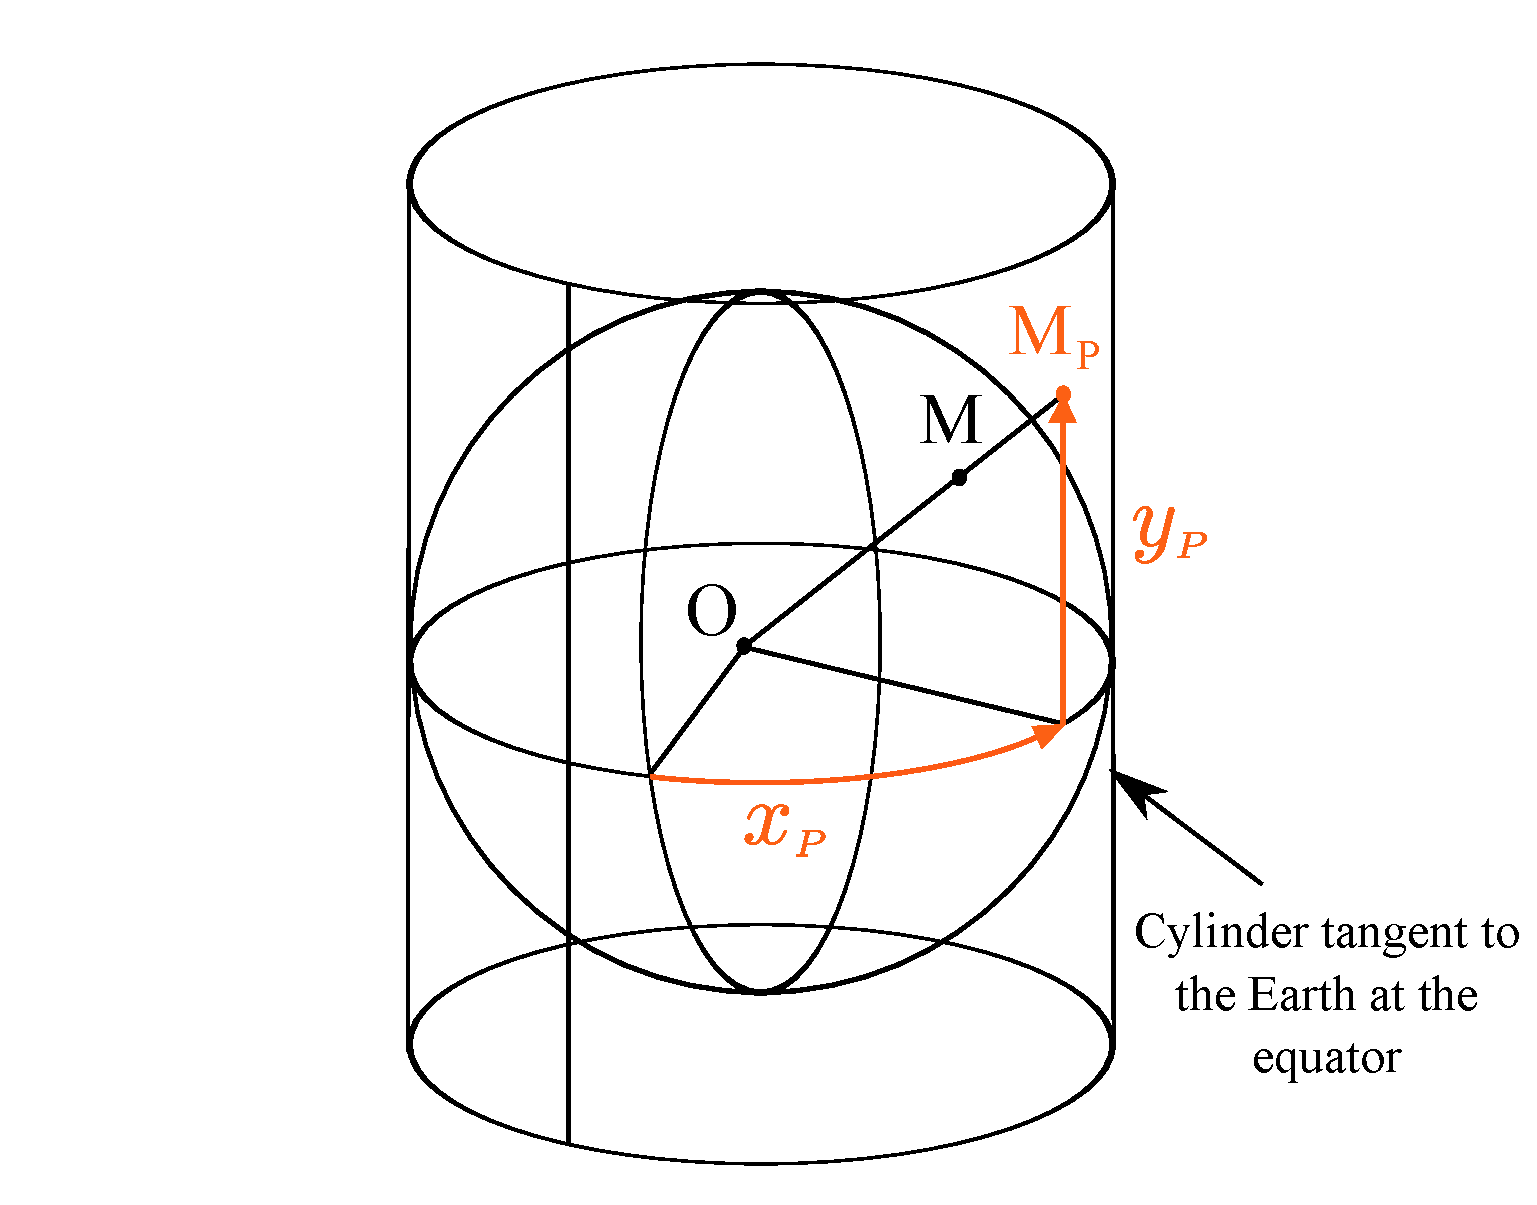
\includegraphics[scale=0.4]
  {graphics/mercator.pdf}%
  \caption{Sketch of the first phase of the Mercator projection (this figure is
  inspired by the figure 2.5 in \cite{hervouet007}).}%
  \label{figure5}%
\end{figure}
% EndExpansion

The coordinates $x_{p}$ and $y_{p}$ on this plane are deduced from the
geographical coordinates by:%
\[x_{p}=R\,\varphi\]
\[y_{p}=R\tan(\lambda)\]
However, the coordinates written in this referential do not correspond to a
conformal projection because:

\begin{itemize}
\item for an east--west displacement, $dx$, on the surface of the Earth, we
  obtain a displacement $dx_{p}$ in this referential such as:
\end{itemize}
\begin{equation}
  dx=\cos(\lambda)\,dx_{p}%
\end{equation}
\begin{itemize}
\item while for a north--south displacement, $dy$, we obtain a displacement
  $dy_{p}$ such as:
\end{itemize}
\begin{equation}
  dy=\cos^{2}(\lambda)\,dy_{p}%
\end{equation}

This distortion, which is greater in the north--south direction than in the
east--west direction, makes the projection non-conformal. We get a conformal
projection by a simple change of scale in the $y$ direction. The new ordinate
$Y$ is then deduced from $y_{p}$, then from $\lambda$, by:%
\begin{equation}
  dY=\cos(\lambda)\,dy_{p}=\dfrac{R}{\cos(\lambda)}d\lambda
\end{equation}
Moreover, it is possible to carry out a change in the origin at one point
$(\varphi_{0},\lambda_{0})$. Along the horizontal axis we immediately obtain:%
\begin{equation}
  X=R(\varphi-\varphi_{0})
\end{equation}
Along the vertical axis, we obtain by integration:%
\begin{equation}
  Y=R\left(  \ln\left[  \tan\left(  \dfrac{\lambda}{2}+\dfrac{\pi}{4}\right)
    \right]  -\ln\left[  \tan\left(  \dfrac{\lambda_{0}}{2}+\dfrac{\pi}{4}\right)
    \right]  \right)
\end{equation}
These coordinates $X$ and $Y$ are coordinates taken on maps and input to the
software for numerical simulation. Hence, one should know how to express the
Navier--Stokes equations in these coordinates. $X$ and $Y$ being functions of
spherical coordinates, it is therefore practical to express the equations in
these spherical coordinates at the very beginning. For this, we use the
divergence and gradient operators expressed in these coordinates:%
\begin{equation}
  \Div \vec{F}=\dfrac{1}{R\cos(\lambda)}\dfrac{\partial F_{\varphi}}%
  {\partial\varphi}+\dfrac{1}{R\cos(\lambda)}\dfrac{\partial(F_{\lambda}%
    \cos(\lambda))}{\partial\lambda}%
\end{equation}
%
\begin{equation}
  \vec{grad}(f)=\dfrac{1}{R\cos(\lambda)}\dfrac{\partial f}%
  {\partial\varphi}\vec{e}_{\varphi}+\dfrac{1}{R}\dfrac{\partial f}{\partial
    \lambda}\vec{e}_{\lambda}%
\end{equation}

Given the nature of the physical quantities and of the projection, the scalar
and vectorial quantities (depth, velocity) are unchanged. We have for example
$F_{\varphi}=F_{x}$ and $F_{\lambda}=F_{y}$.
The derivatives of the functions with respect to $\varphi$ and $\lambda$ are
then replaced by the derivatives along $X$ and $Y$, the Mercator coordinates:%
\begin{equation}
  \dfrac{\partial f}{\partial\varphi}=\dfrac{\partial f}{\partial X}\dfrac{\partial
    X}{\partial\varphi}+\dfrac{\partial f}{\partial Y}\dfrac{\partial Y}%
  {\partial\varphi}=R\dfrac{\partial f}{\partial X}%
\end{equation}
%
\begin{equation}
  \dfrac{\partial f}{\partial\lambda}=\dfrac{\partial f}{\partial X}\dfrac{\partial
    X}{\partial\lambda}+\dfrac{\partial f}{\partial Y}\dfrac{\partial Y}%
  {\partial\lambda}=\dfrac{R}{\cos(\lambda)}\dfrac{\partial f}{\partial Y}%
\end{equation}

From this, new expressions of divergence%
\index{divergence}
and gradient%
\index{gradient}
are deduced:%
\begin{align}
  \Div \vec{F}  &  =\dfrac{1}{\cos(\lambda)}\dfrac{\partial F_{x}}{\partial
    X}+\dfrac{1}{\cos(\lambda)}\dfrac{\partial F_{y}}{\partial Y}-\dfrac{\tan
    (\lambda)}{R}F_{y}\nonumber\\
  &  =\dfrac{1}{\cos^{2}(\lambda)}\dfrac{\partial}{\partial X}(F_{x}\cos
  (\lambda))+\dfrac{1}{\cos^{2}(\lambda)}\dfrac{\partial}{\partial Y}(F_{y}%
  \cos(\lambda))
\end{align}
%
\begin{equation}
  \Grad(f)=\dfrac{1}{\cos(\lambda)}\left(
    \begin{array}
      [c]{c}%
      \dfrac{\partial f}{\partial X}\\
      \dfrac{\partial f}{\partial Y}%
    \end{array}
  \right)
\end{equation}
The equations could be solved by using all these formulae, but, in finite
elements, this would induce a problem with the approximation space. As a matter
of fact, if $\lambda$ is a polynomial function, what becomes of $\cos
(\lambda)$? If $\cos(\lambda)$ and $\sin(\lambda)$ are polynomials, what is
$\tan(\lambda)$? These questions are fundamental when mass conservation has to
be proved.

Now,\ if we take \textit{e.g.} a conservative advection equation:%
\begin{equation}
  \dfrac{\partial f}{\partial t}+\Div(f\,\vec{u})=0
\end{equation}
it becomes in Mercator projection:%
\begin{equation}
  \dfrac{\partial(f\cos^{2}(\lambda))}{\partial t}+\Div(\cos(\lambda)f\,\vec{u})=0
\end{equation}
where $\Div$ is now the Cartesian divergence operator.
We shall see that integration into the Mercator domain of this equation will
give terms such as:%
\[\dfrac{\partial}{\partial t}\int\nolimits_{\Omega}f\cos^{2}(\lambda
)\,dXdY\,\,\text{\thinspace\ and}\,\,\,\,\int\nolimits_{\Omega}\Div(f\,\vec
{u}\cos(\lambda)\,)\,dXdY\,\,\]
this last term being equal to:%
\[\,\int\nolimits_{\Gamma}f\,\vec{u}\,.\,\vec{n}\,\cos(\lambda)\,d\Gamma\]
In these terms, each length $dX$, $dY$ or $d\Gamma$\ is multiplied by
$\cos(\lambda)$, which restores a real local scale. The volumes or flux
calculated are thus real quantities. In the same way, the gradient terms would
give real slopes.
As in the case of all operators, the coordinates therefore appear multiplied
by $\cos(\lambda)$. The idea is to carry out this operation once and for all
before the start of calculations. This can be formalised by choosing a
constant latitude $\lambda$ per element. The advantage is that the equations
to be worked out are then strictly identical to the Cartesian equations (this
is actually due to the local character of the operators and is not a general
property). This choice of constant latitude per element is naturally an
approximation, but it enables us to retain strict finite element formalism,
the approximation being somehow transferred to the coordinates.
During a computation using spherical coordinates with a meshing in the
Mercator projection, we shall build up a set of coordinates multiplied by
$\cos(\lambda)$. If we use the coordinates modified in this manner, the
Mercator projection is naturally taken into consideration and no other
modification appears again in the Navier-Stokes equations. All the mass and
flow calculations are coherent and provide real values.
The error in taking a constant latitude per element can be evaluated by
finding the form which the Navier-Stokes equations should take with the
coordinates $X^{\prime}$ and $Y^{\prime}$ such as $X^{\prime}=X\,\cos
(\lambda)$ and $Y^{\prime}=Y\,\cos(\lambda)$. The difference at the continuum
level between the equations makes the ignored terms, which are of the order of
$1/R$, appear. They take into consideration the variations in latitude within
the element.

\begin{CommentBlock}{Important note by J.-M. Hervouet:}
  The multiplication of coordinates of the points by the cosine of a
  constant latitude per element leads to a paradoxical situation: a point which
  belongs to several elements has as many sets of different coordinates which
  should be stored element by element. In fact this does not constitute a technical
  problem and does not lead to any contradiction. All calculations of vectors or
  matrices in finite elements start at the elementary level, where coherence is
  required only between the coordinates of the points of the element. It should
  even be possible, without any topological problem, to build a
  \textquotedblleft two-dimensional\textquotedblright\ meshing of the Earth for
  calculating world tides, each element having coordinates corresponding to a
  local projection (the poles should be excluded, however, having infinite coordinates
  in Mercator projection).
\end{CommentBlock}
